\documentclass[
size=17pt,
paper=smartboard,
mode=present,
display=slidesnotes,
style=paintings,
nopagebreaks,
blackslide,
fleqn]{powerdot}

% styles: sailor, paintings
% wj capsules prettybox
% mode = handout or present


\usepackage{amsmath,graphicx,color,amsfonts}
\usepackage[brazilian]{babel}
\usepackage[utf8]{inputenc}
\newcommand{\palette}{Moitessier}


% palettes:
%    - sailor: Sea, River, Wine, Chocolate, Cocktail 
%    - paintings: Syndics, Skater, GoldenGate, Moitessier, PearlEarring, Lamentation, HolyWood, Europa, MayThird, Charon 

\newcommand{\cursopequeno}{EC01039 CG\underline{PI}}
\newcommand{\cursogrande}{\Large EC01039 -- Computação gráfica e \underline{processamento de imagem}}



\author{Ronaldo de Freitas Zampolo\\FCT-ITEC-UFPA}
\date{2020.2}


\pdsetup{
	lf = {\cursopequeno},
	rf = {Filtragem}, 
	cf = {\arabic{slide}~/~\pageref*{lastslide}},
	palette = {\palette}, 
	randomdots={false}
}

%opening
\title{\cursogrande\\ \vspace{1cm}Filtragem}
\author{Ronaldo de Freitas Zampolo\\FCT-ITEC-UFPA}
%\date{ }

\begin{document}
   \maketitle[randomdots={false}]
   \begin{slide}{Agenda}
      \tableofcontents[content=sections]
   \end{slide}

\section[ slide = true]{Filtragem espacial}
   \begin{slide}[toc=]{Fundamentos}
      \begin{itemize}
       \item Filtro: aceitar ou rejeitar (selecionar) determinados componentes de frequência
       \item Sistemas LI: caracterizados pela resposta ao impulso $h(x,y)$
       \begin{itemize}
          \item Máscara
          \item Kernel
          \item Template
          \item Janela
       \end{itemize}
       \begin{align*}
          g(x,y) &= h(x,y)\ast f(x,y)\\
                 &= \sum_{s=-a}^{a}\sum_{t= -b}^{b} f(s,t)h(x-s,y-t) 
       \end{align*}
       \item Filtragem não linear também pode ser implementada (Ex.: filtro de mediana para redução de ruído impulsivo)
      \end{itemize}
   \end{slide}

   \begin{slide}[toc=]{Funcionamento (filtragem espacial linear)}
      \begin{center}
          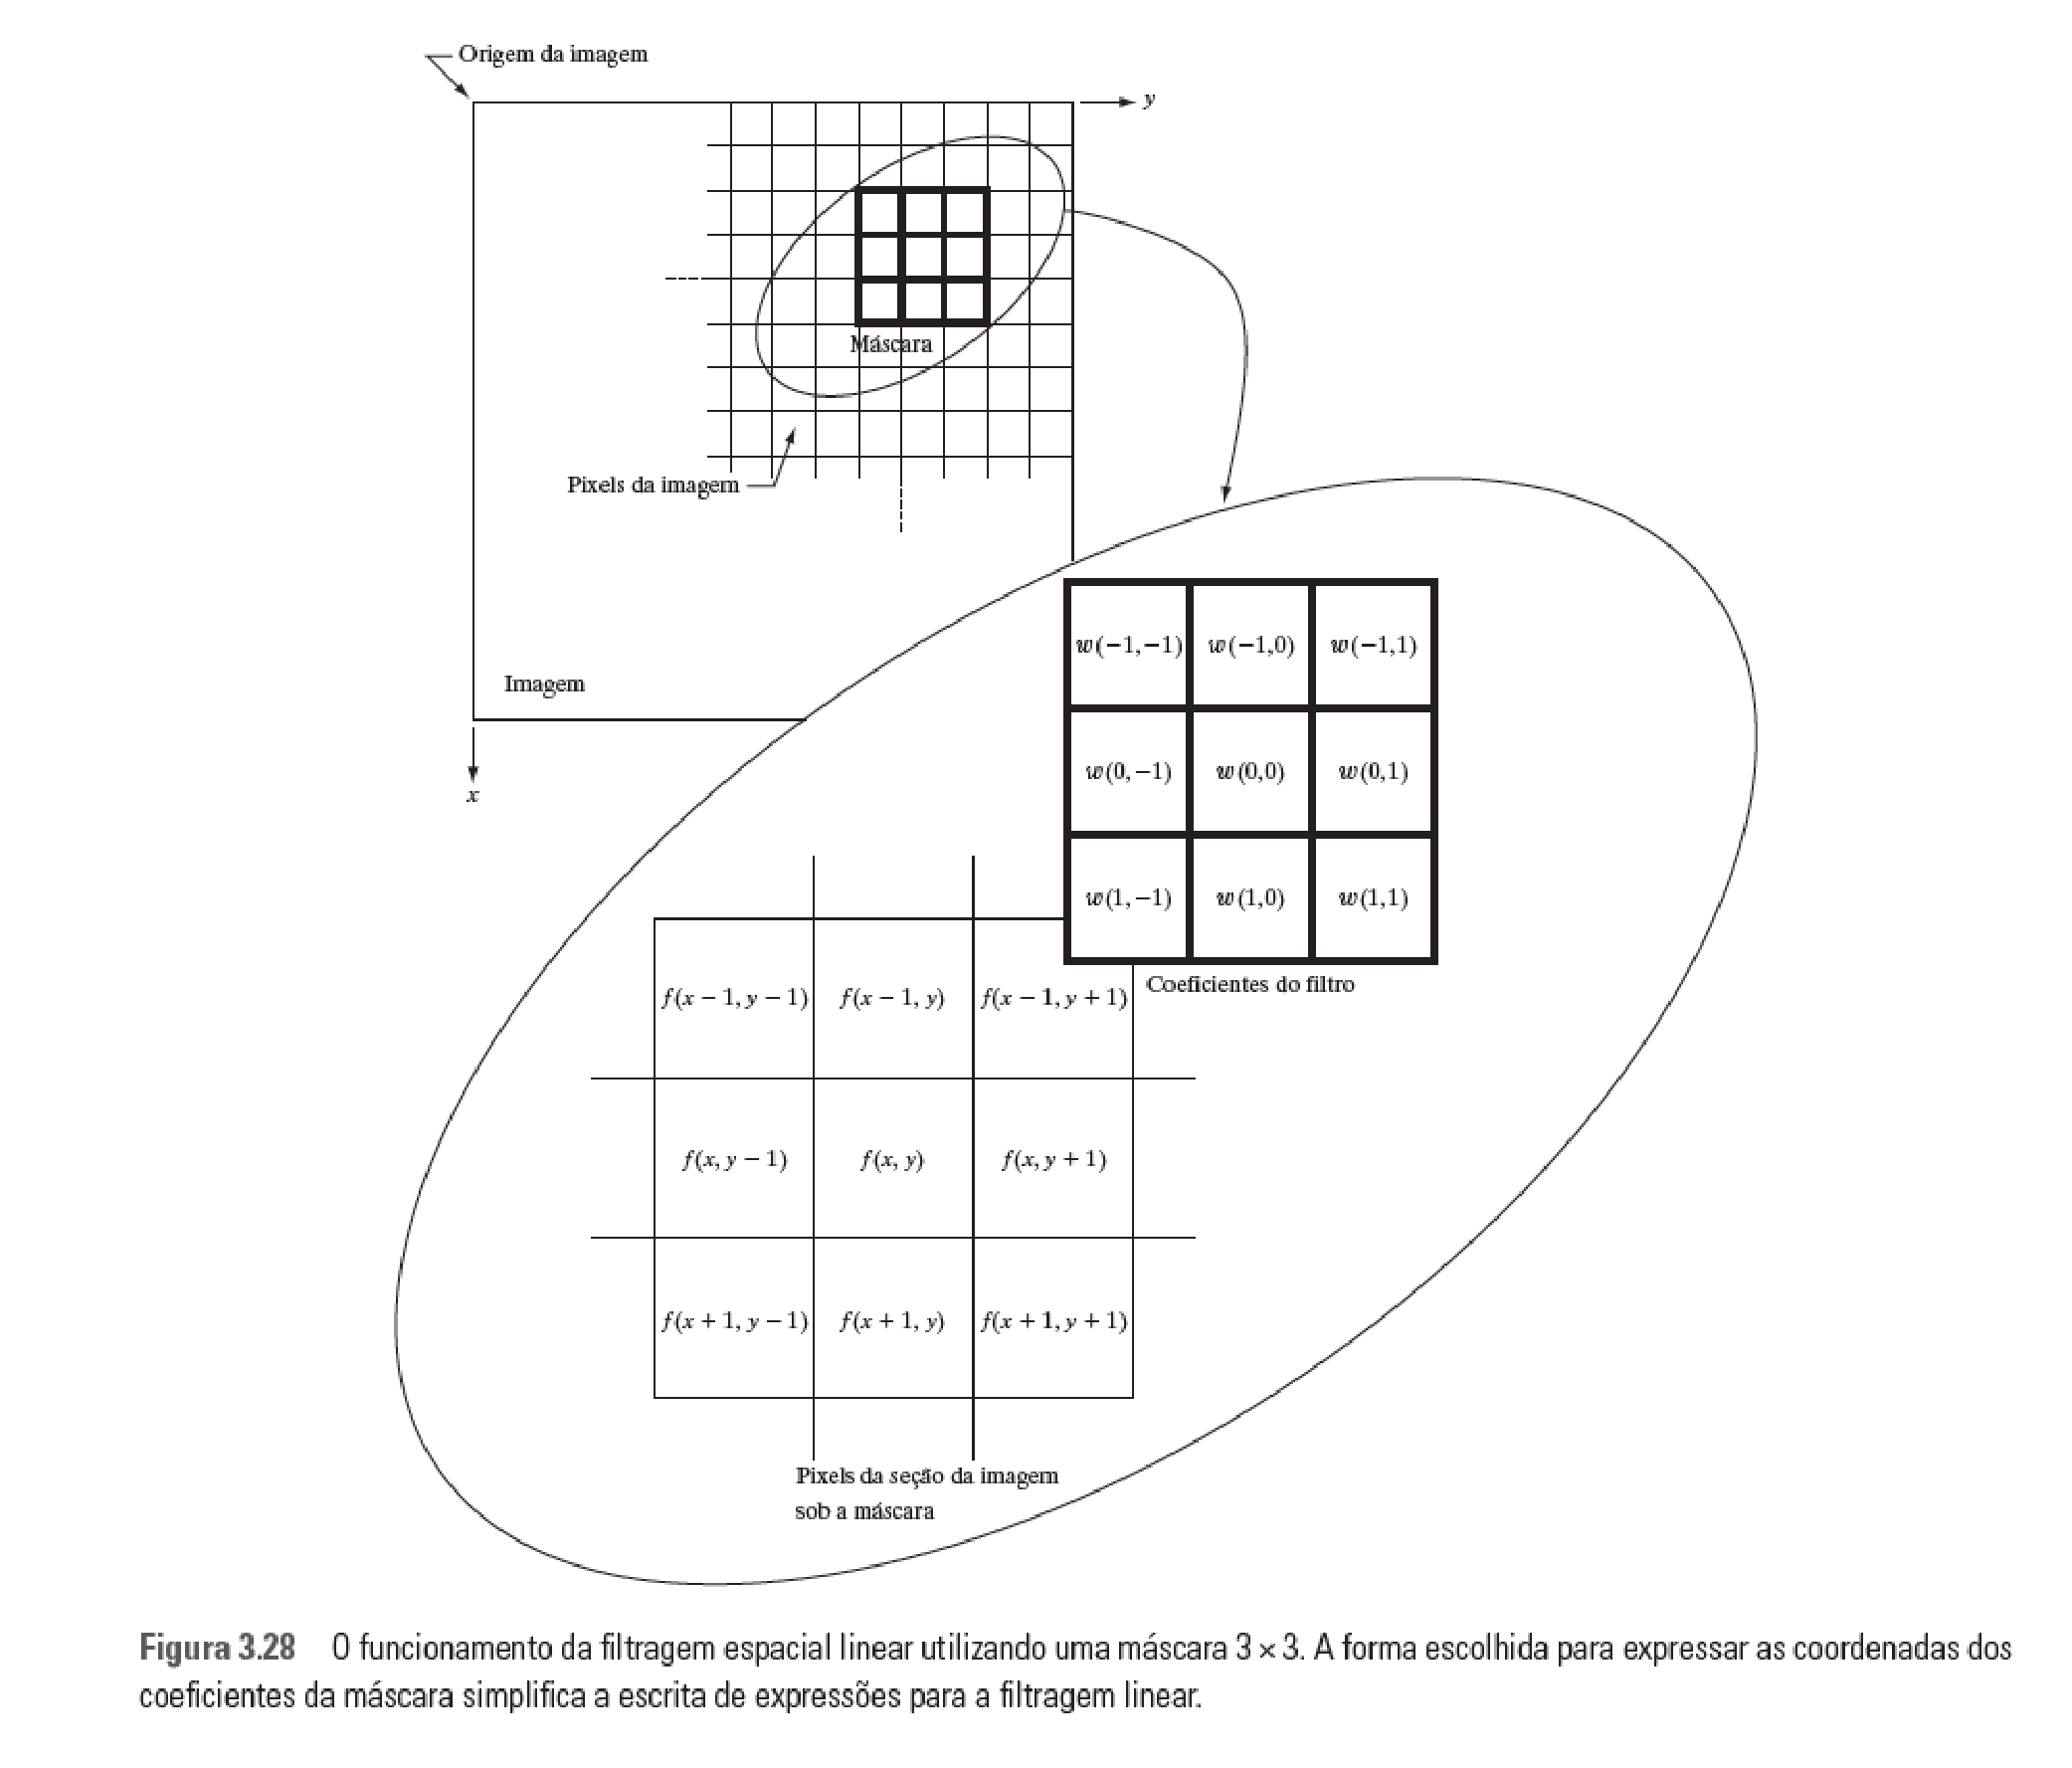
\includegraphics[width=0.65\textwidth]{figs/fig0328}
      \end{center}
   \end{slide}
   
   \section[ slide = true]{Filtros de suavização}
      \begin{slide}[toc=]{Filtros lineares}
         \begin{itemize}[type=1]
            \item Filtros usados para borramento e redução de ruído (filtros passa-baixa)
            \item Filtro 2D uniforme: \begin{equation*}h(x,y)=\begin{cases}\frac{1}{(2L+1)^2},& -L\leq x\leq L, -L \leq y \leq L\\
                                                           0, & \text{outro caso}\end{cases}\end{equation*}
            \item Filtro gaussiano: 
            \begin{equation*}
               h(x,y)=A \exp\left \{\frac{(x-x_0)^2}{2\sigma_x^2}+\frac{(y-y_0)^2}{2\sigma_y^2}\right\}
            \end{equation*}
            Na prática, $h(x,y)$ precisará ser limitado em $(x,y)$, sendo a constante $A$ calculada de maneira a  
            \begin{equation*}
               \sum_{(x,y)}h(x,y) = 1
            \end{equation*}
         \end{itemize}
      \end{slide}
      
      \begin{slide}[toc=]{Filtros lineares}
      \begin{itemize}
       \item Dois exemplos de máscaras
       \begin{center}
          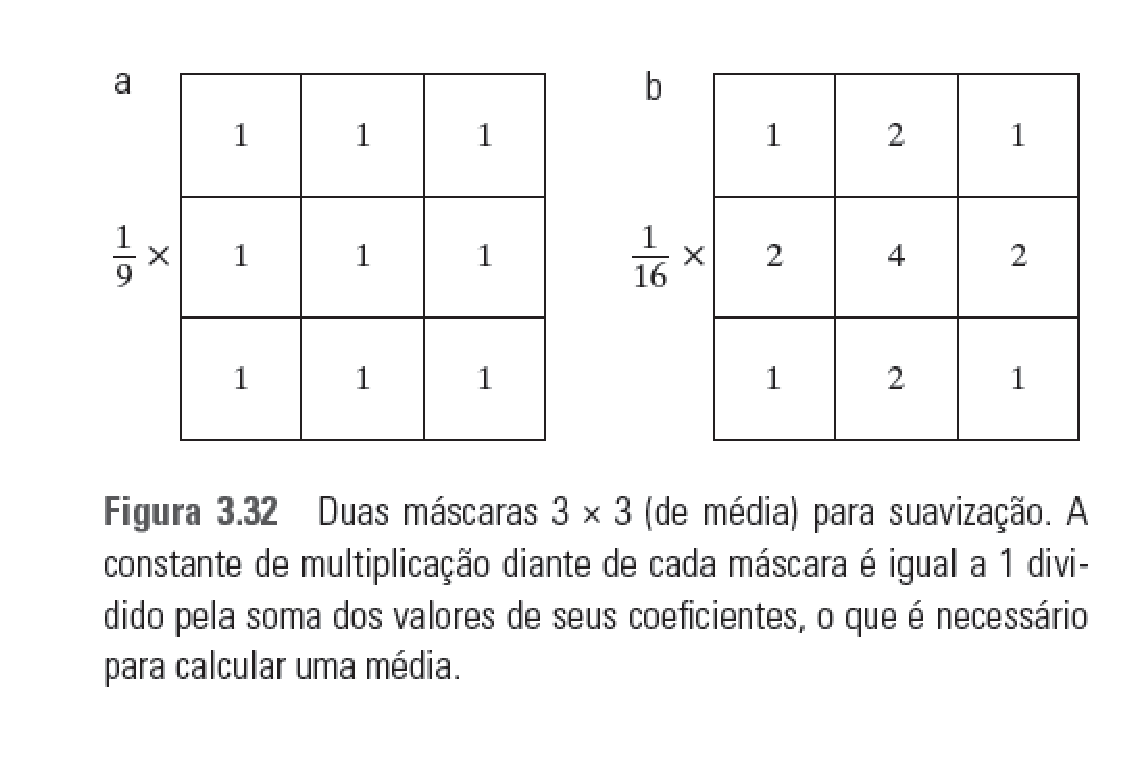
\includegraphics[width=0.7\textwidth]{figs/fig0332}
      \end{center}
      \end{itemize}
      \end{slide}
      
      \begin{slide}[toc=]{Filtros lineares}
      \begin{itemize}
       \item Filtragem 2D uniforme (variação de tamanho do filtro)
       \begin{center}
          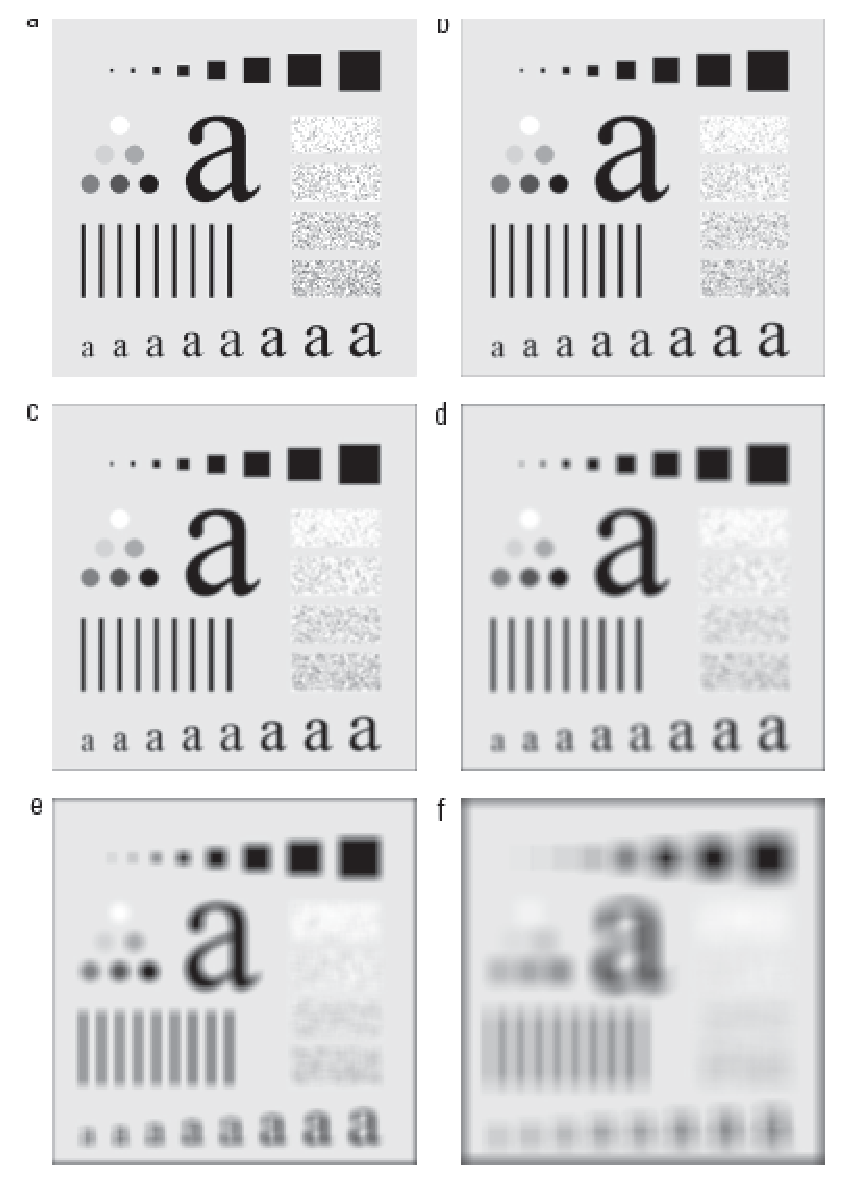
\includegraphics[height=0.7\textheight]{figs/fig0333}
      \end{center}
      \end{itemize}
      \end{slide}
      
      \begin{slide}[toc=]{Filtros lineares}
      \begin{itemize}
       \item Combinação de filtragem linear com transformação de intensidade
       
      \end{itemize}
      \begin{center}
          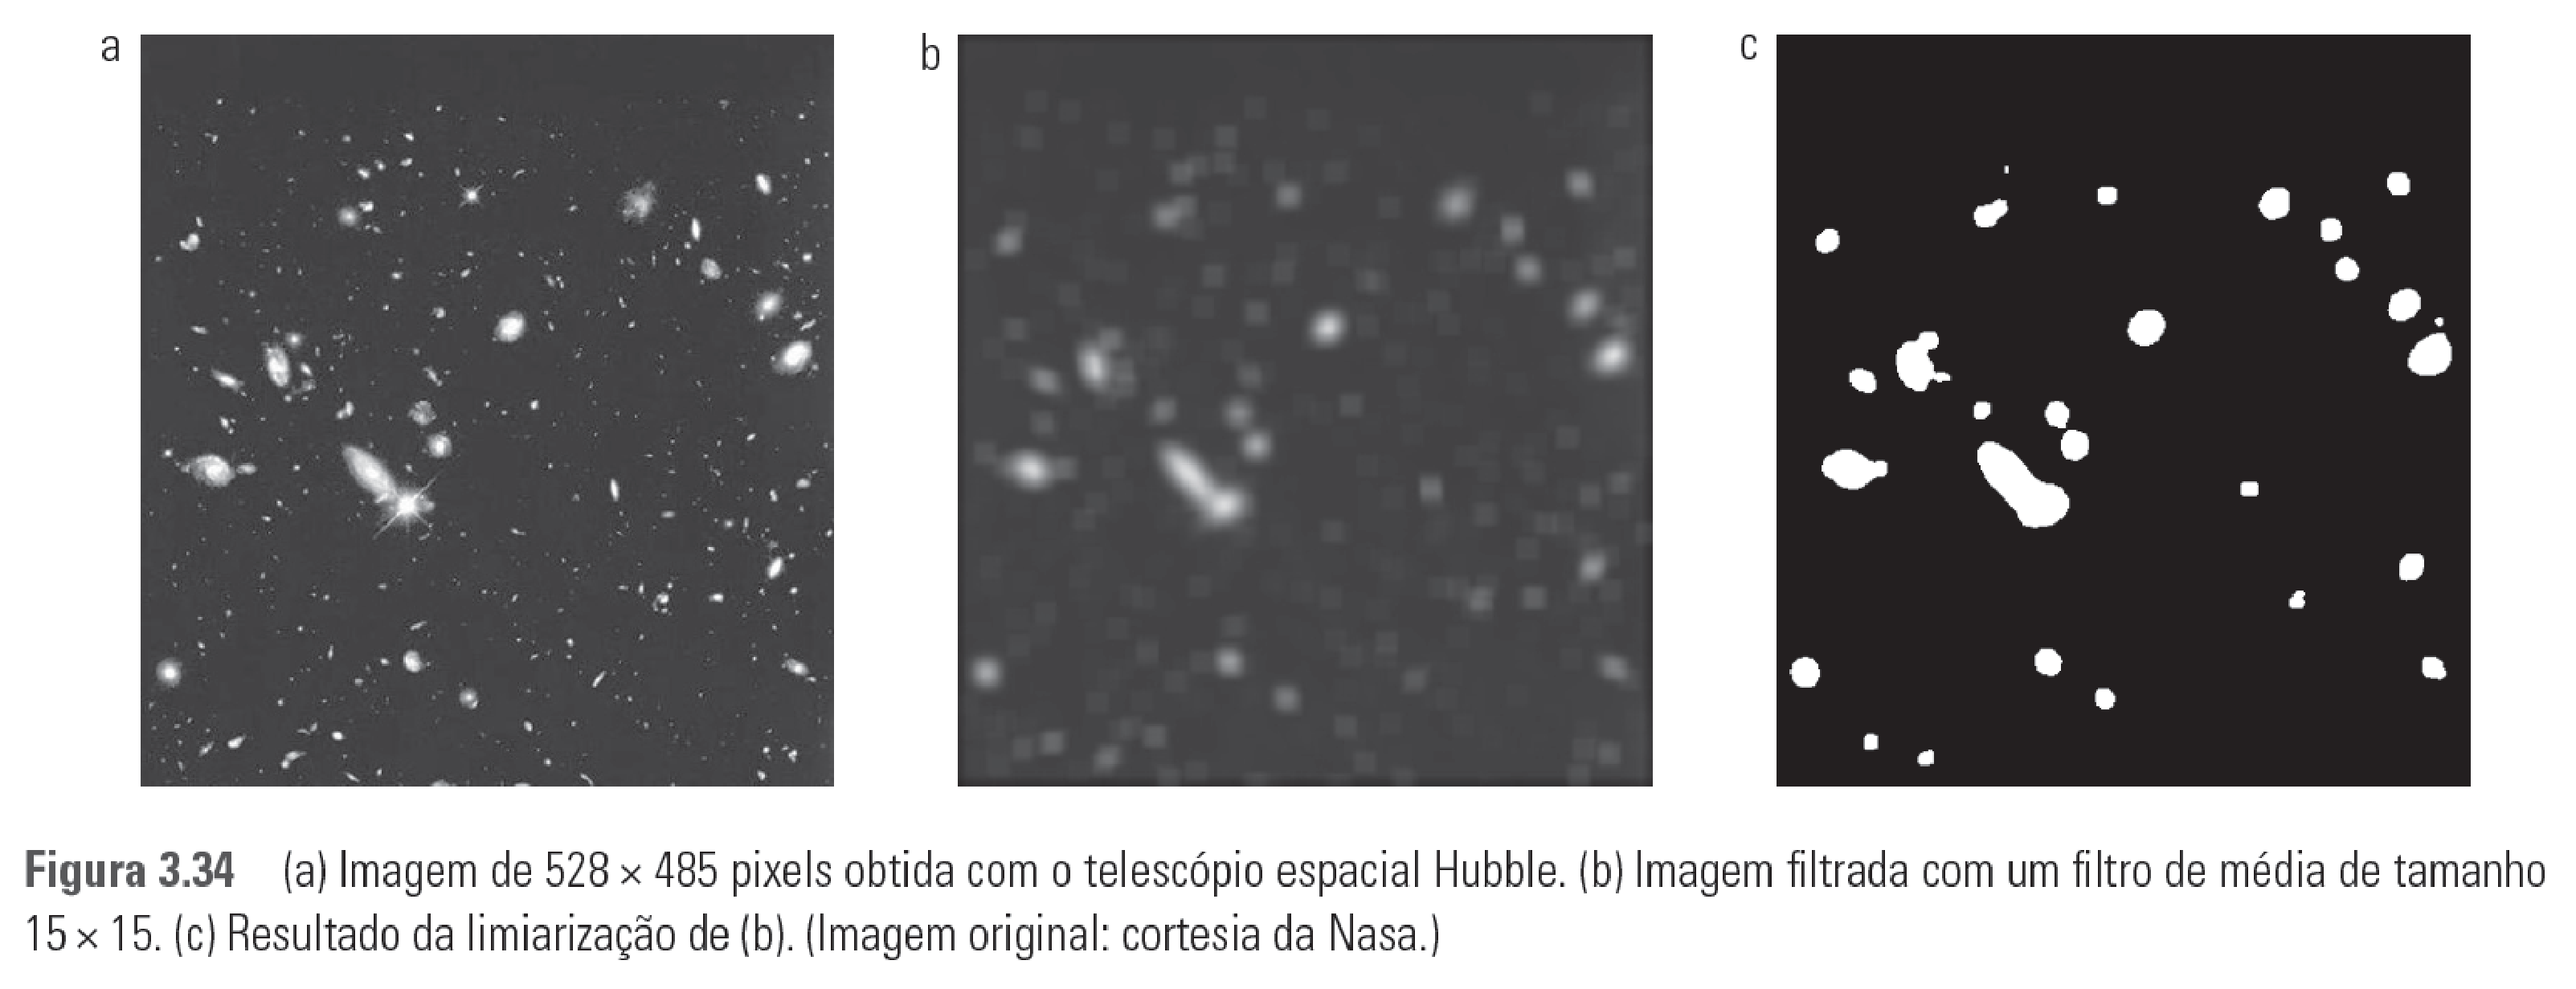
\includegraphics[width=\textwidth]{figs/fig0334}
      \end{center}
      \end{slide}

      \begin{slide}[toc=]{Filtros não lineares}
         \begin{itemize}[type=1]
            \item Filtro de mediana: 
            \begin{equation*}
               g(x,y)=\text{mediana de }\Phi(x,y)
            \end{equation*}
            onde $\Phi(x,y)$ corresponde a uma região da imagem de entrada $f$ em torno do ponto $(x,y)$.\\ \vspace{0.5cm}Qual o efeito desse tipo de operação em uma imagem contaminada por ruído impulsivo?
            \item Comparação de abordagens para eliminação de ruído impulsivo
         \begin{center}
          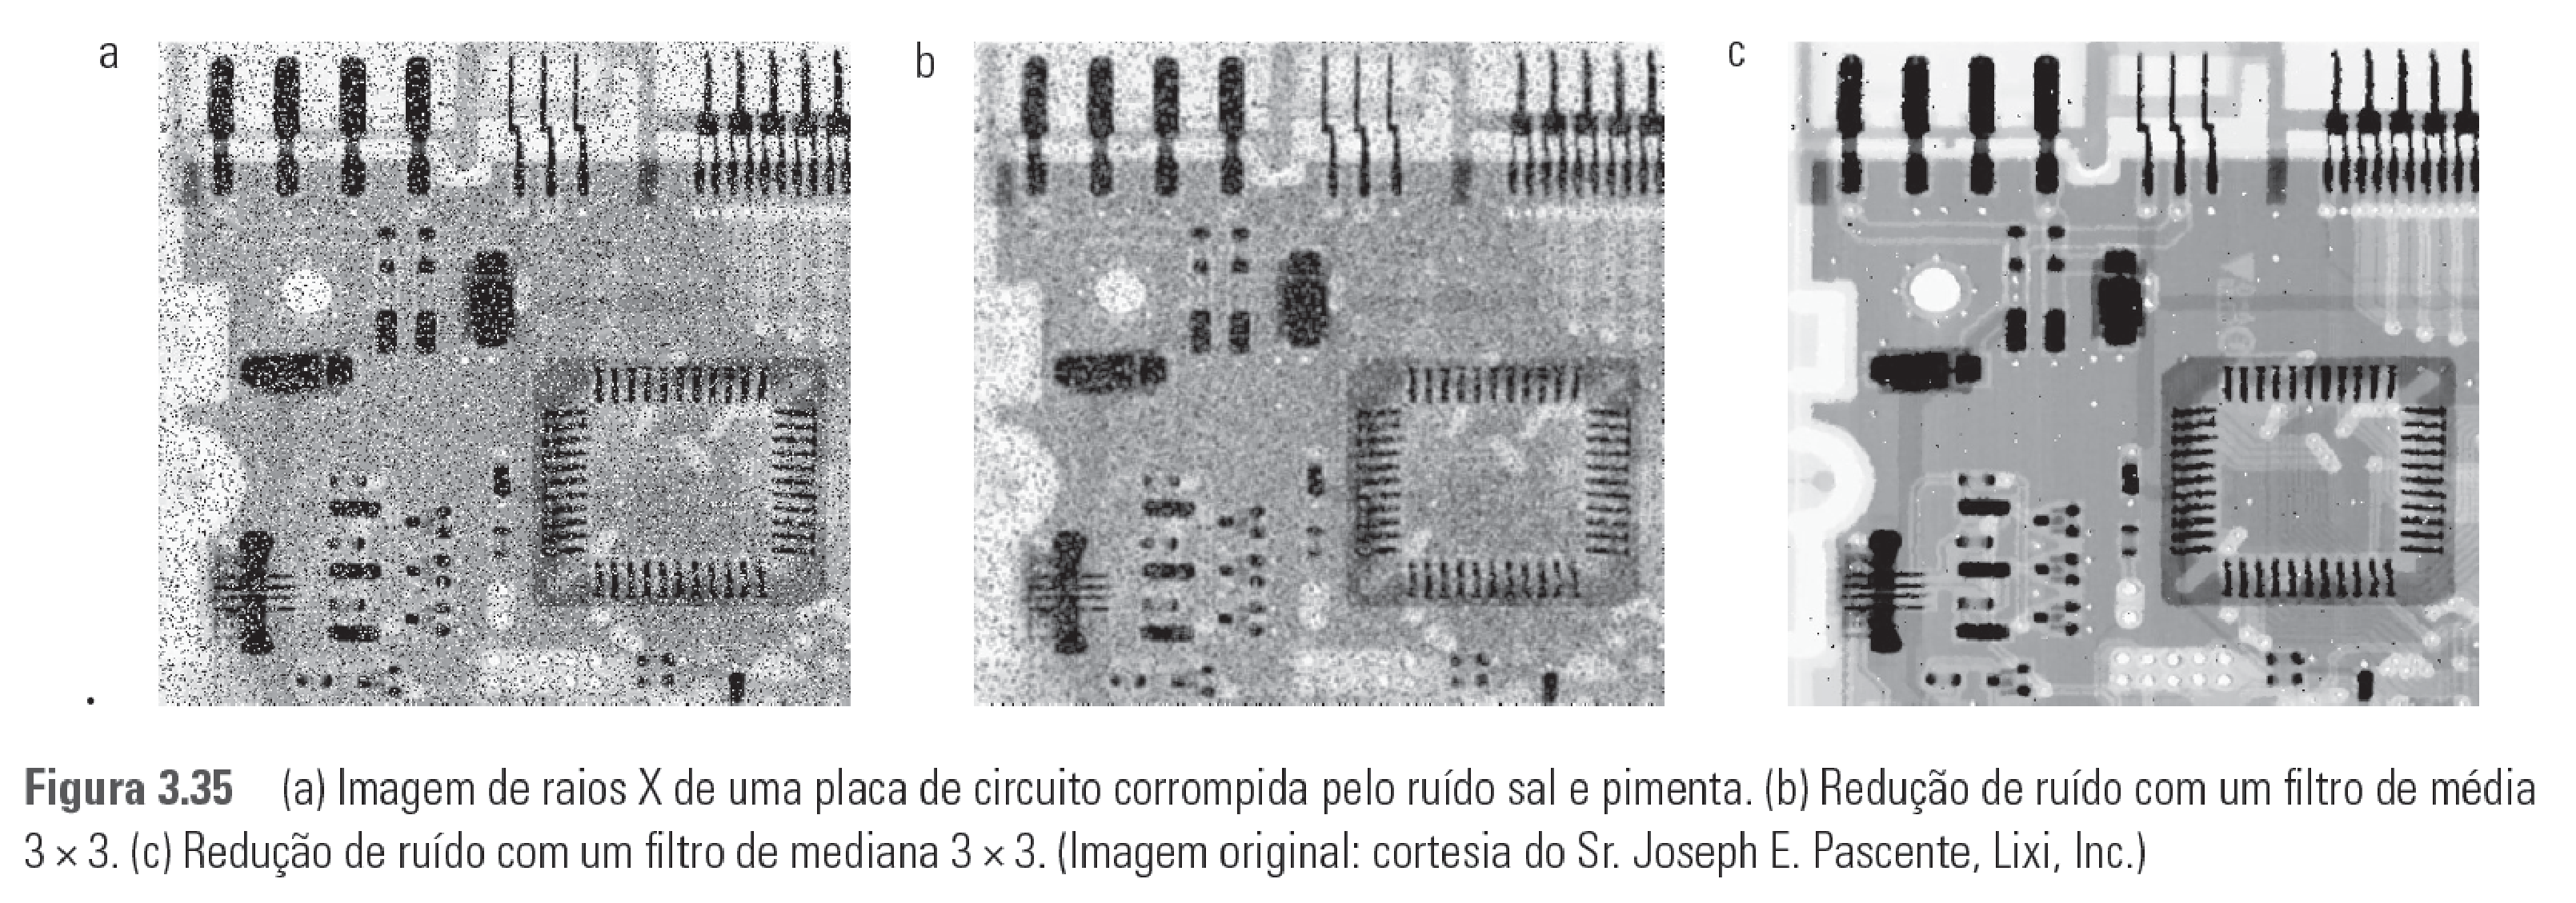
\includegraphics[width=0.7\textwidth]{figs/fig0335}
      \end{center}
         \end{itemize}
      \end{slide}
      
   \section[ slide = true]{Filtros de aguçamento}
      \begin{slide}[toc=]{Fundamentos}
         \begin{itemize}[type=1]
            \item \underline{Objetivo}: salientar transições de intensidade, aumentar a nitidez
            \item Filtros do tipo passa-alta
            \item São comuns filtros baseados na primeira e na segunda derivadas
            \begin{itemize}
               \item Primeira derivada:
               \begin{equation*}
                  \frac{\partial f(x,y)}{\partial x} = f(x+1,y)-f(x,y)
               \end{equation*}
               
               \item Segunda derivada:
               \begin{equation*}
                  \frac{\partial^2 f(x,y)}{\partial x^2} = f(x+1,y)+f(x-1,y)-2f(x,y)
               \end{equation*}
            \end{itemize}
         \end{itemize}
      \end{slide}
      
      \begin{slide}[toc=]{Exemplo em perfil da aplicação da primeira e segunda derivadas}
      \begin{center}
          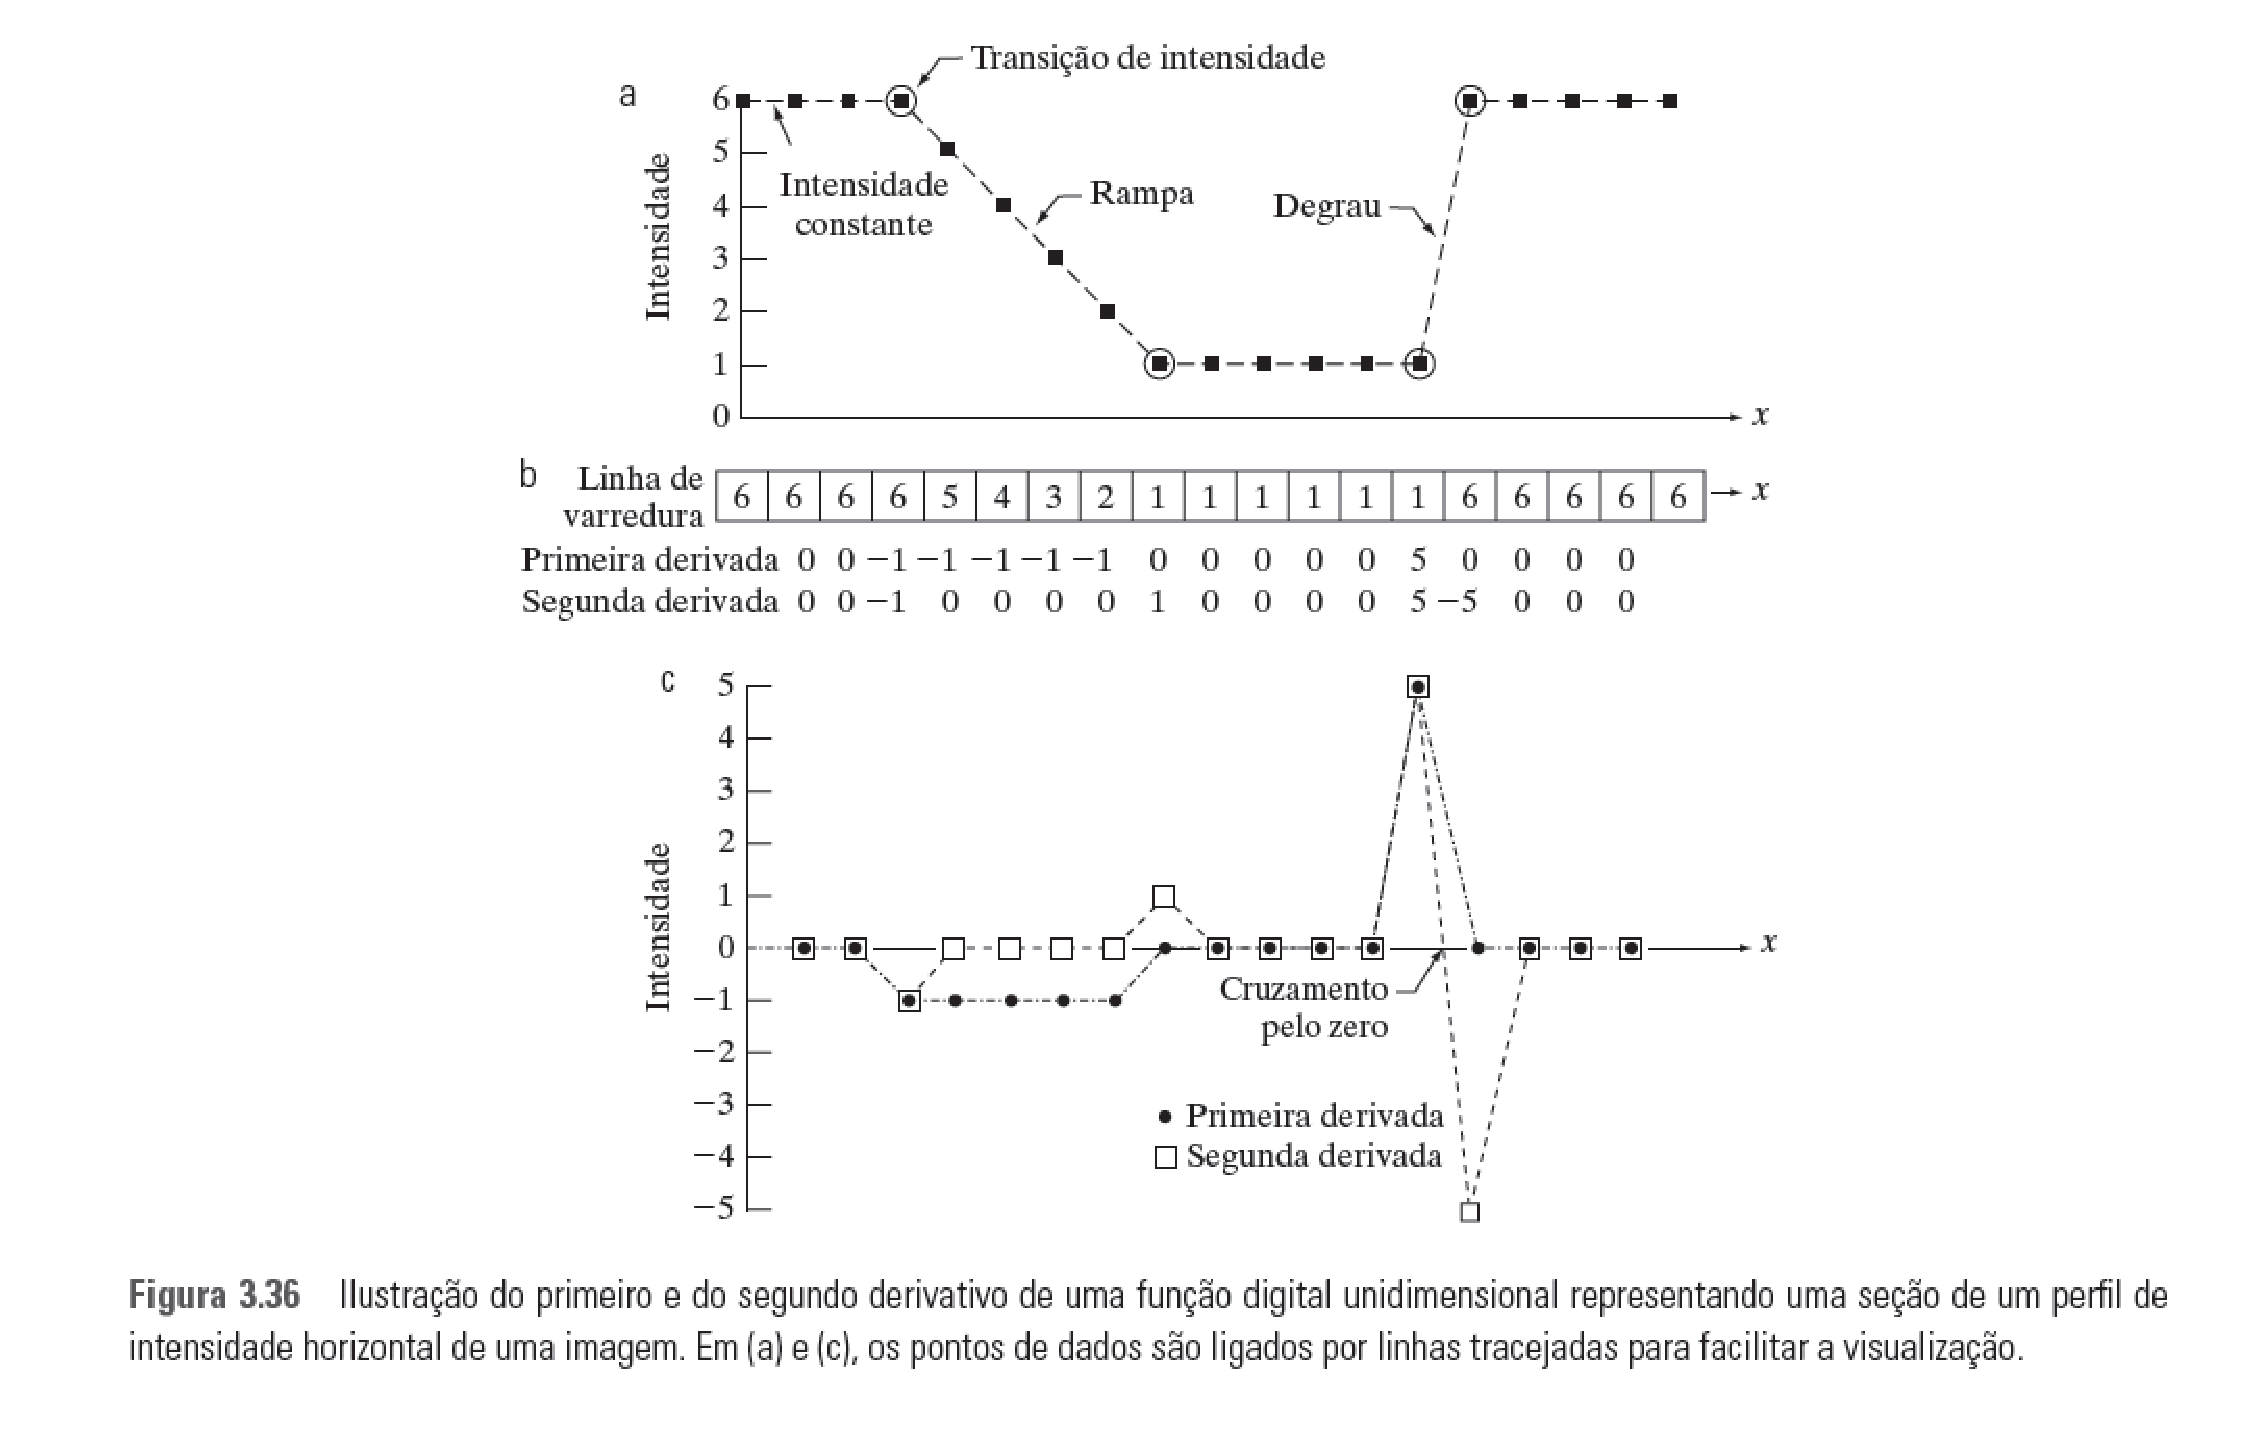
\includegraphics[width=.85\textwidth]{figs/fig0336}
      \end{center} 
      \end{slide}
      
      \begin{slide}[toc=]{O Laplaciano}
      \begin{itemize}
         \item \underline{Operador isotrópico} mais simples
         \begin{align*}
            \nabla^2f =& \frac{\partial^2f}{\partial x^2}+\frac{\partial^2f}{\partial y^2}\\
                      =& f(x+1,y)+f(x-1,y)+f(x,y+1)+\\
                       & + f(x,y-1)-4f(x,y)
         \end{align*}
         \item Uso do Laplaciano no aguçamento de imagens
         \begin{equation*}
            g(x,y) = f(x,y) + c\{\nabla^2f(x,y)\}
         \end{equation*}
      \end{itemize}
      \end{slide}
      
      \begin{slide}[toc=]{Máscaras para Laplaciano}
      \begin{center}
          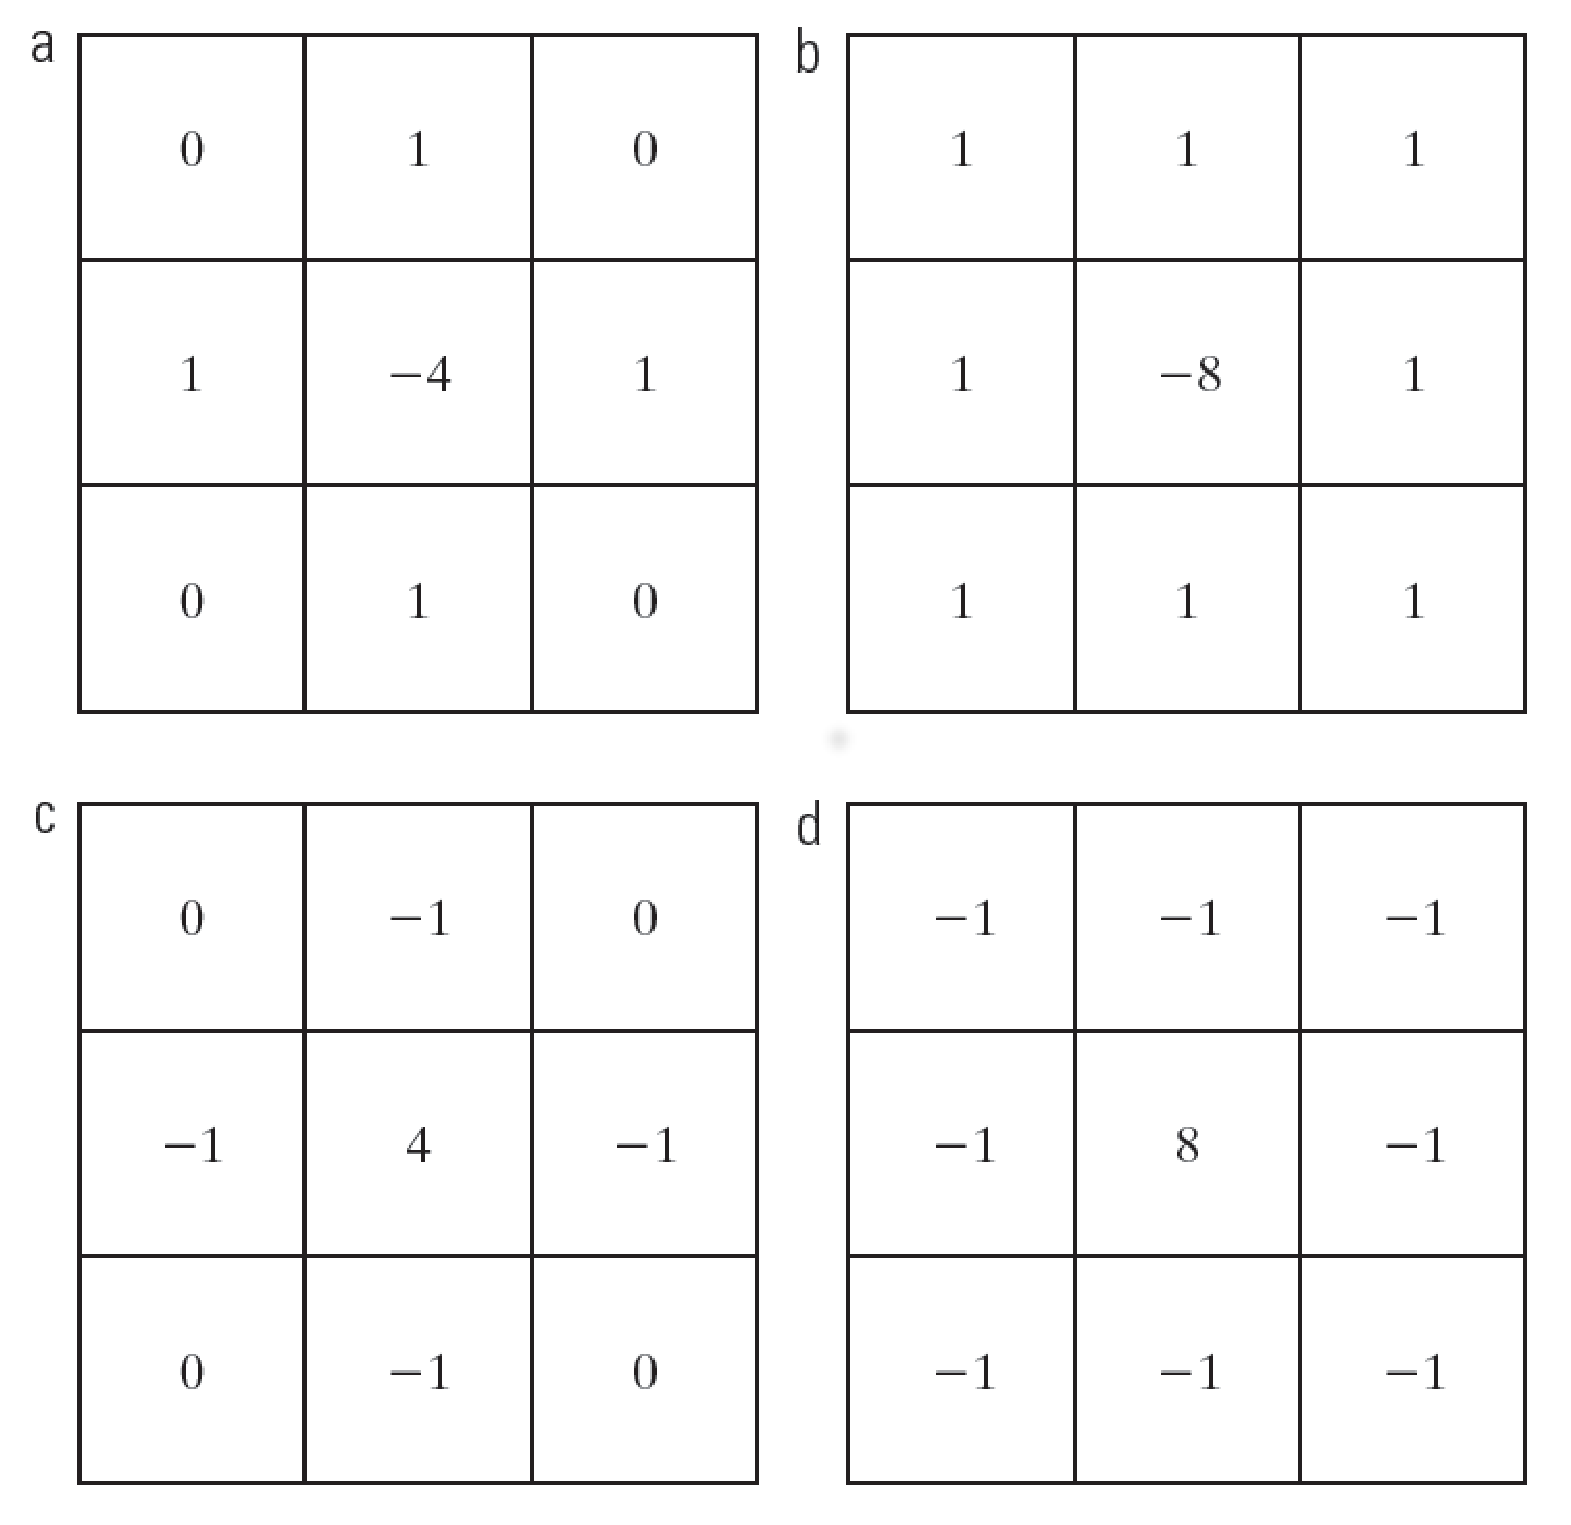
\includegraphics[width=0.55\textwidth]{figs/fig0337}
      \end{center}  
      \end{slide}
      
      \begin{slide}[toc=]{Exemplo de aguçamento}
      \begin{center}
          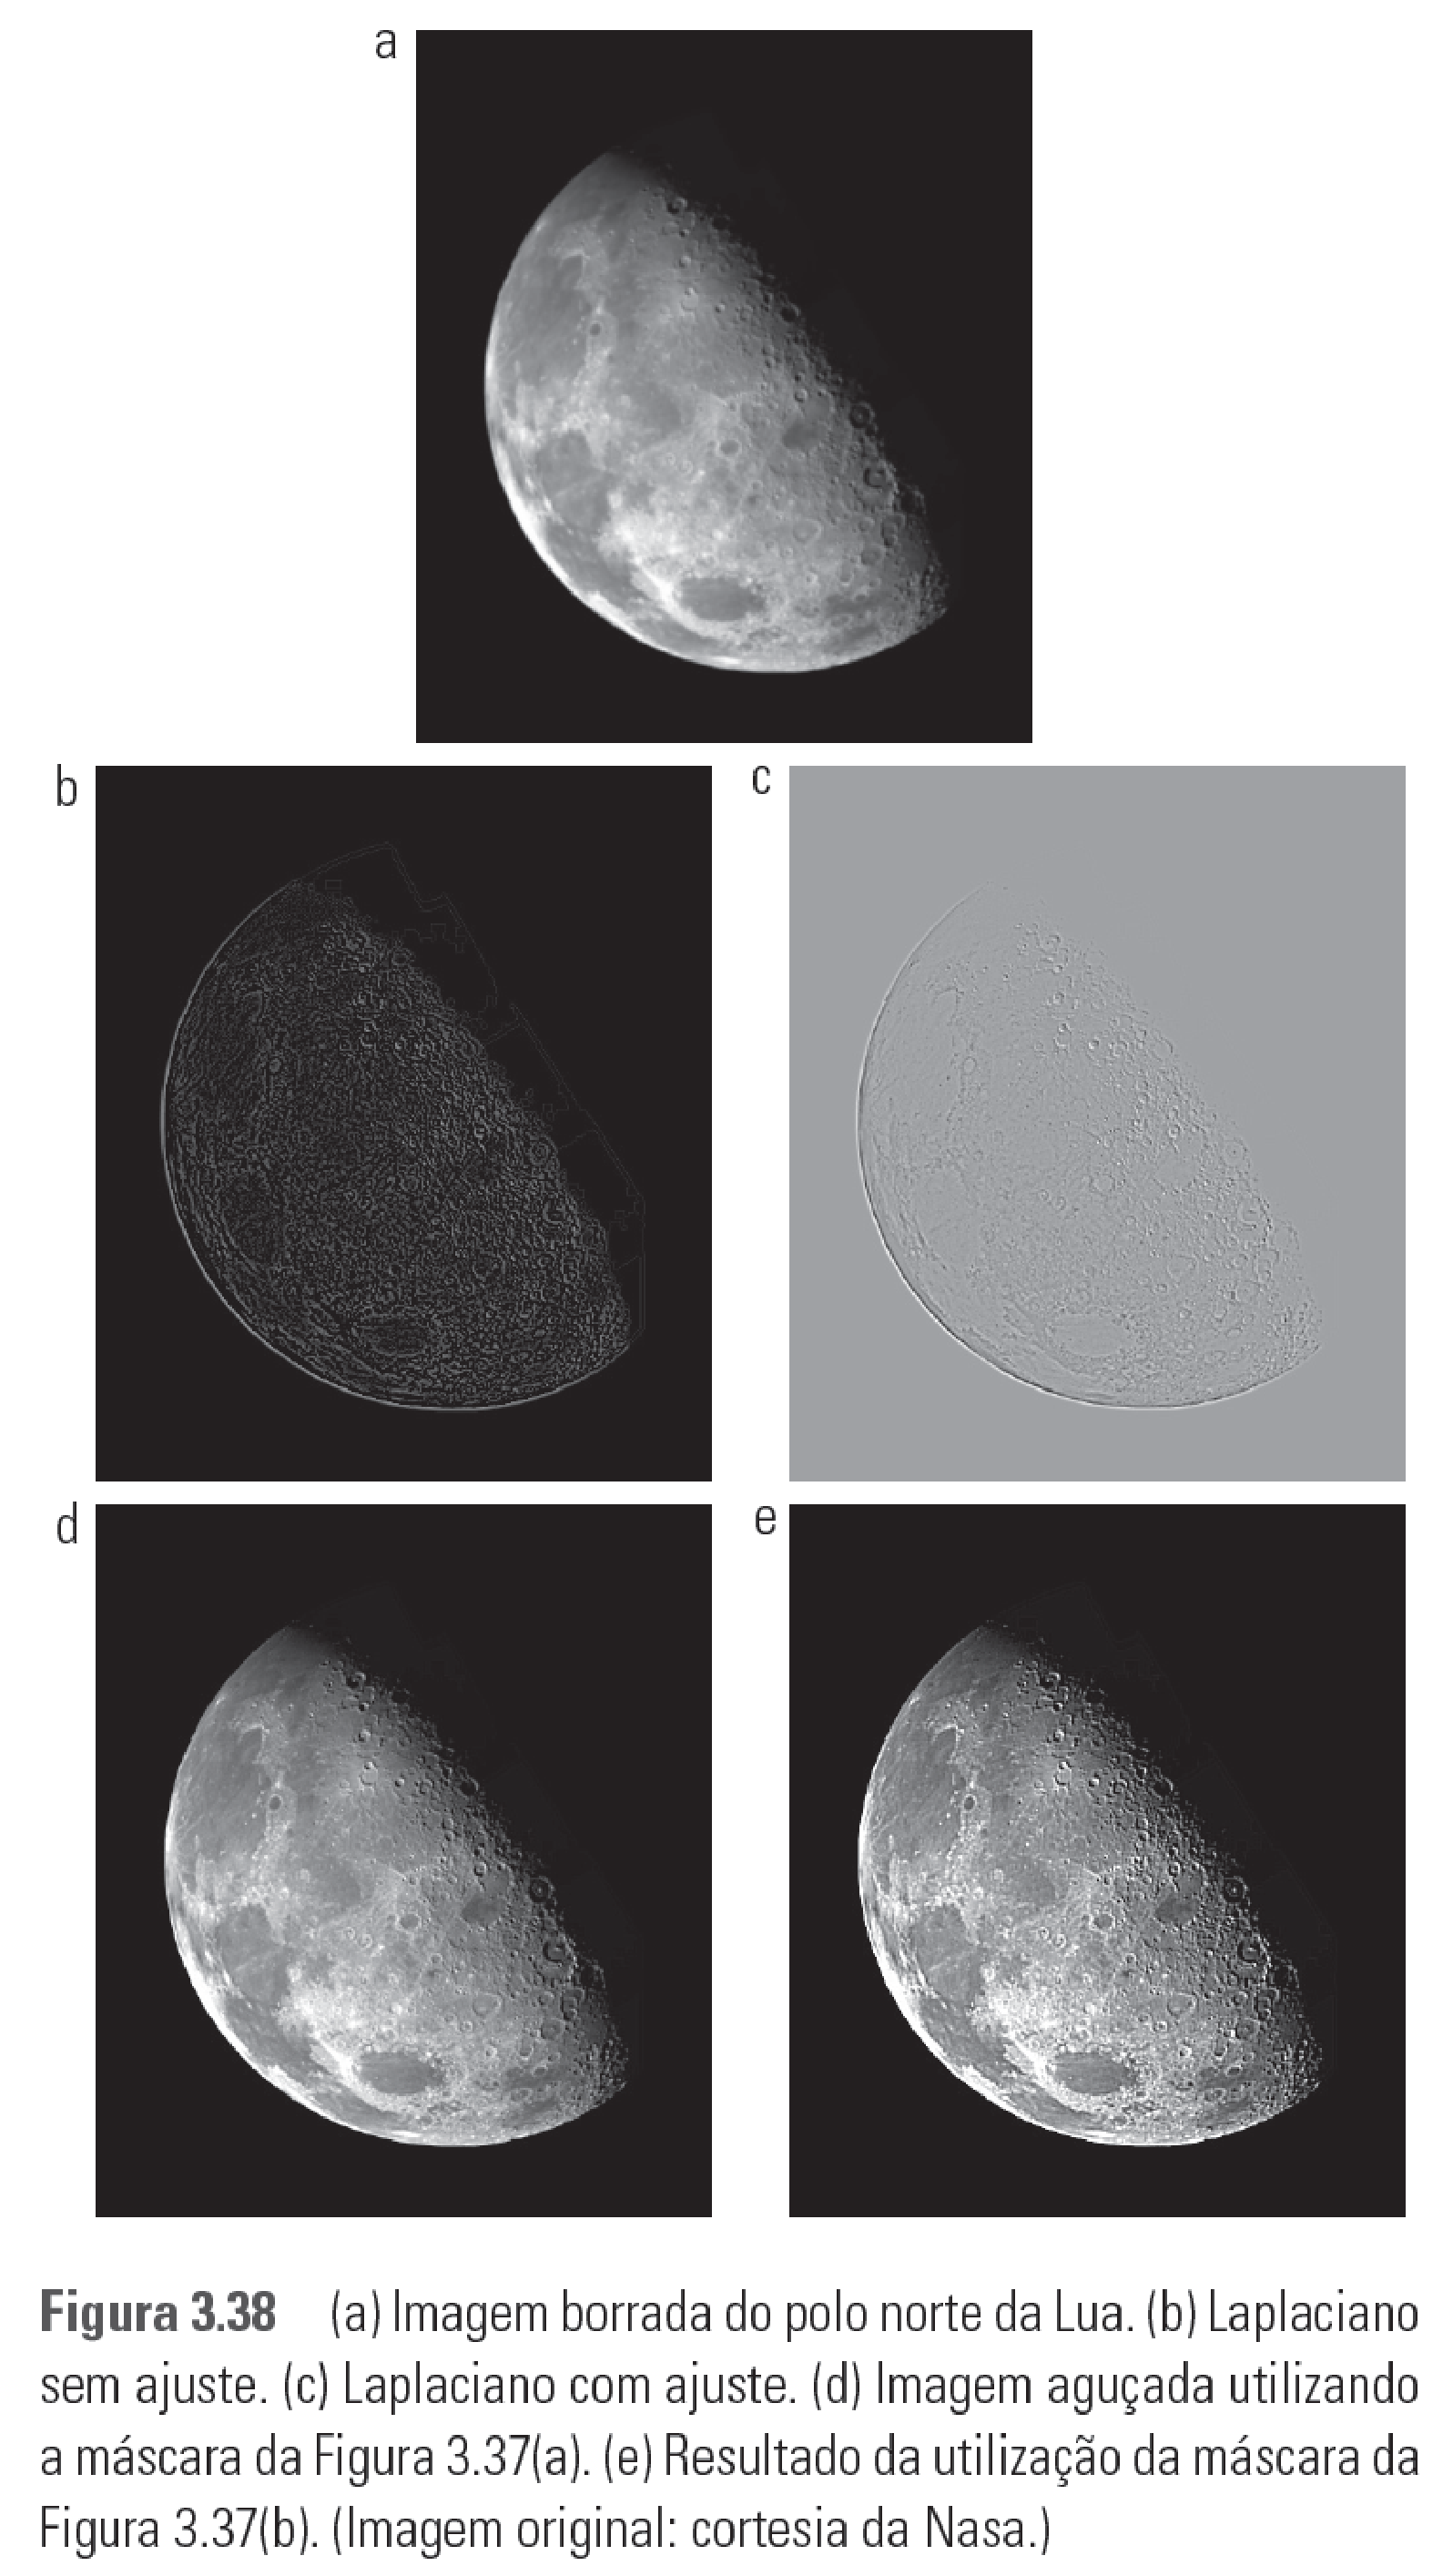
\includegraphics[height=0.75\textheight]{figs/fig0338}
      \end{center}  
      \end{slide}

      \begin{slide}[toc=]{Filtragem high-boost}
         \twocolumn{
         \begin{itemize}[type=1]
            \item Consiste em 
            \begin{itemize}
               \item Borrar a imagem de entrada
               \item Subtrair a imagem borrada da original (máscara)
               \item Adicionar a máscara à imagem de entrada
            \end{itemize}
         \end{itemize}}{
         \begin{center}
          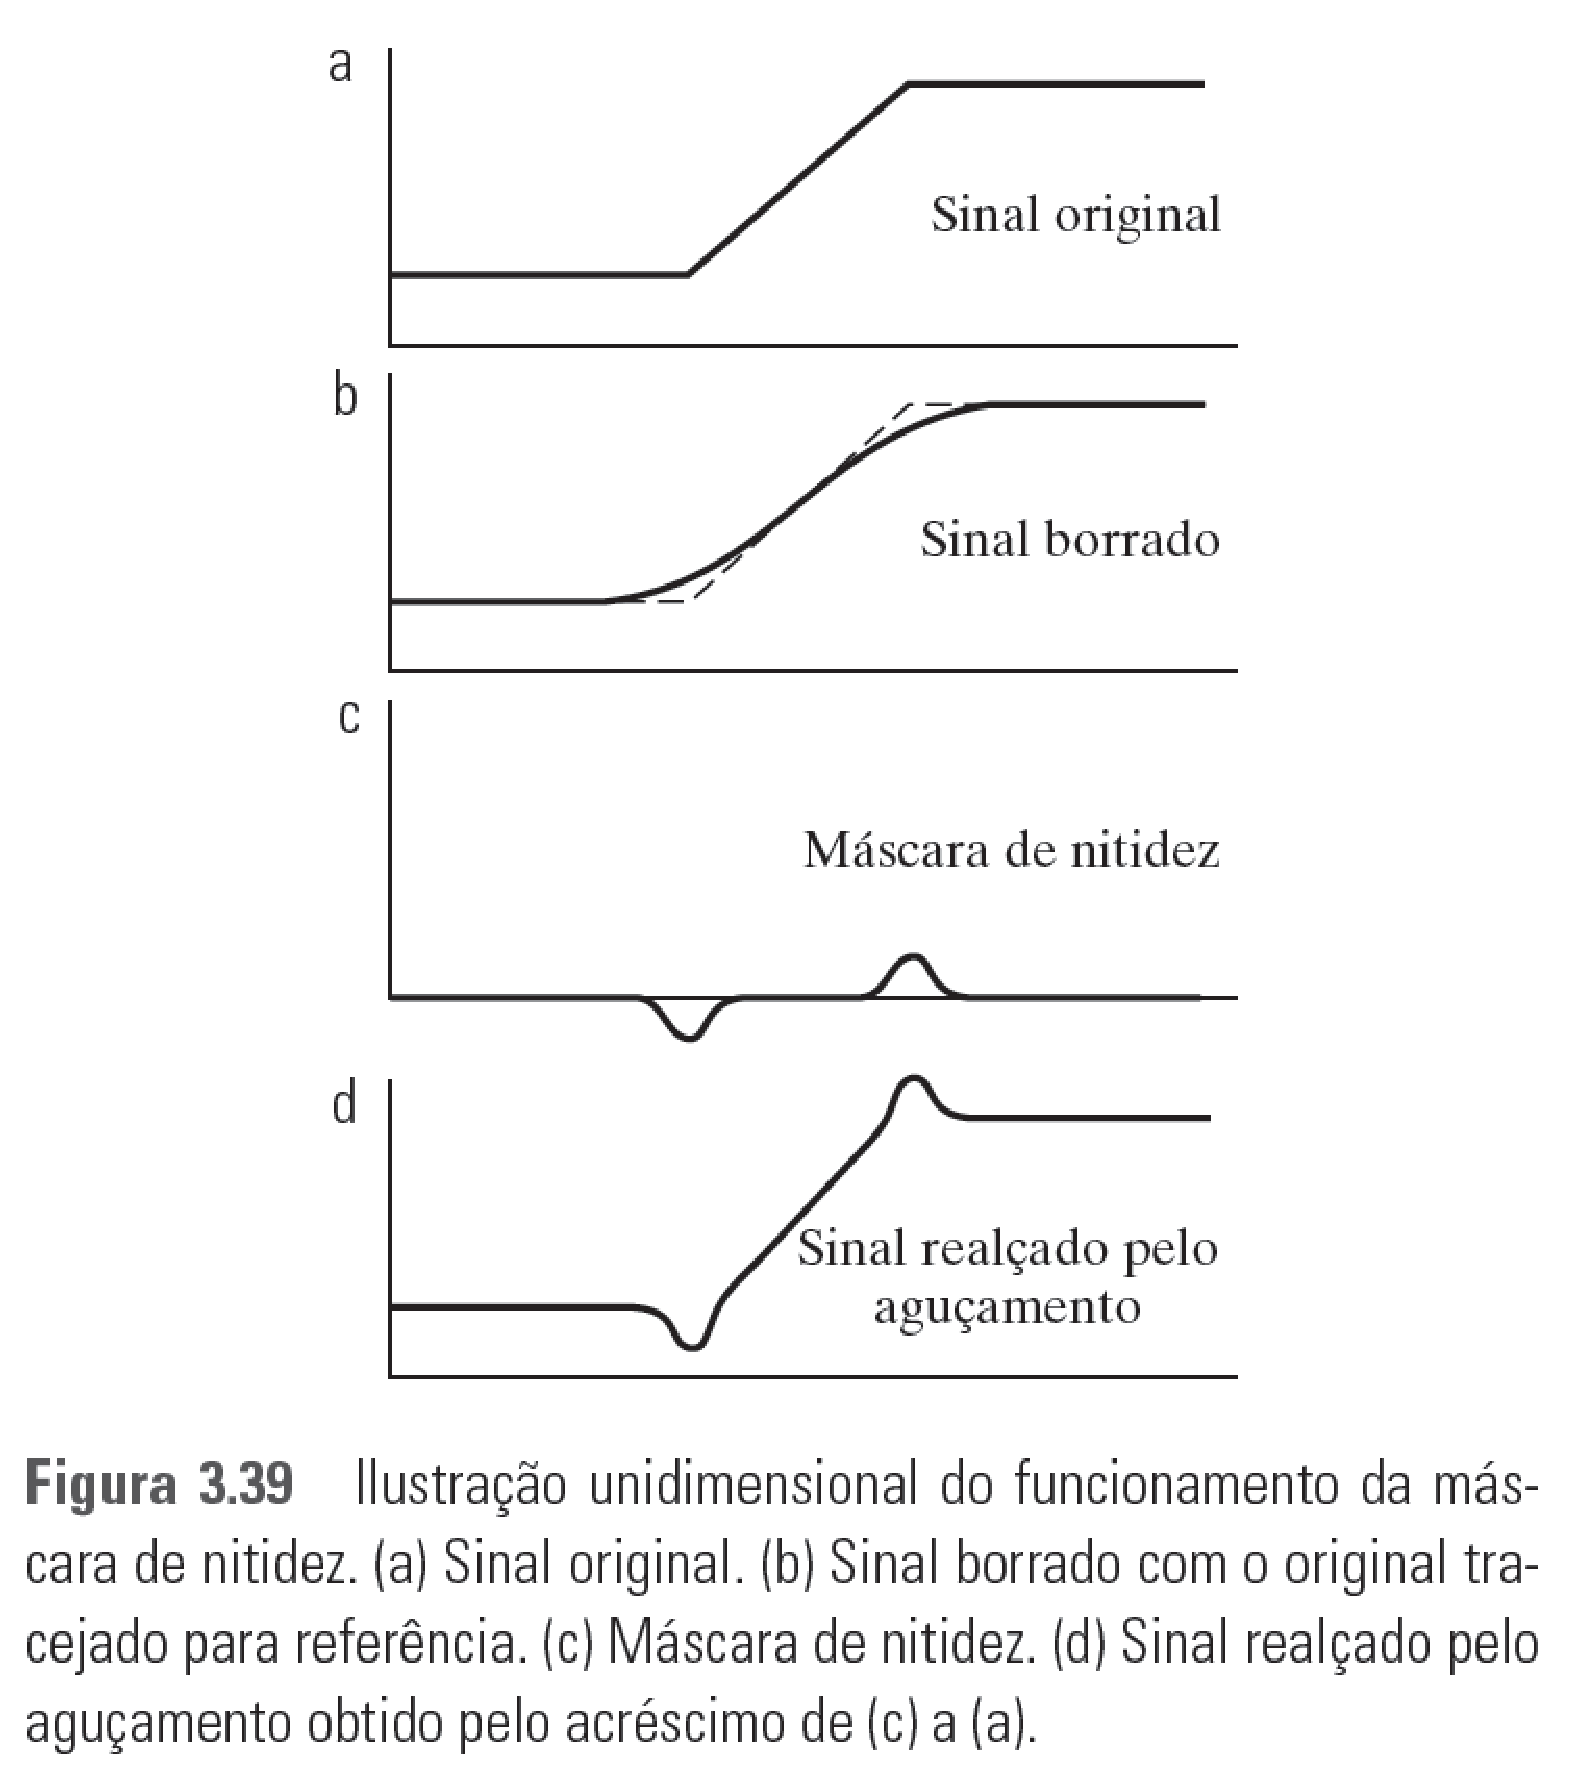
\includegraphics[width=\textwidth]{figs/fig0339}
      \end{center}}
      \end{slide}


\section[ slide = true ]{Representação em frequência: extensões para duas dimensões}
      \begin{slide}[toc=]{Impulso unitário}
         \begin{itemize}[type=1]
            \item O impulso unitário discreto 2D é definido como 
            \begin{equation*}
               \delta(x-x_0,y-y_0) = \begin{cases}
                                1, & \text{se } x=x_0, y=y_0\\
                                0, & \text{caso contrário}
                             \end{cases}
            \end{equation*}
			 \begin{center}
				 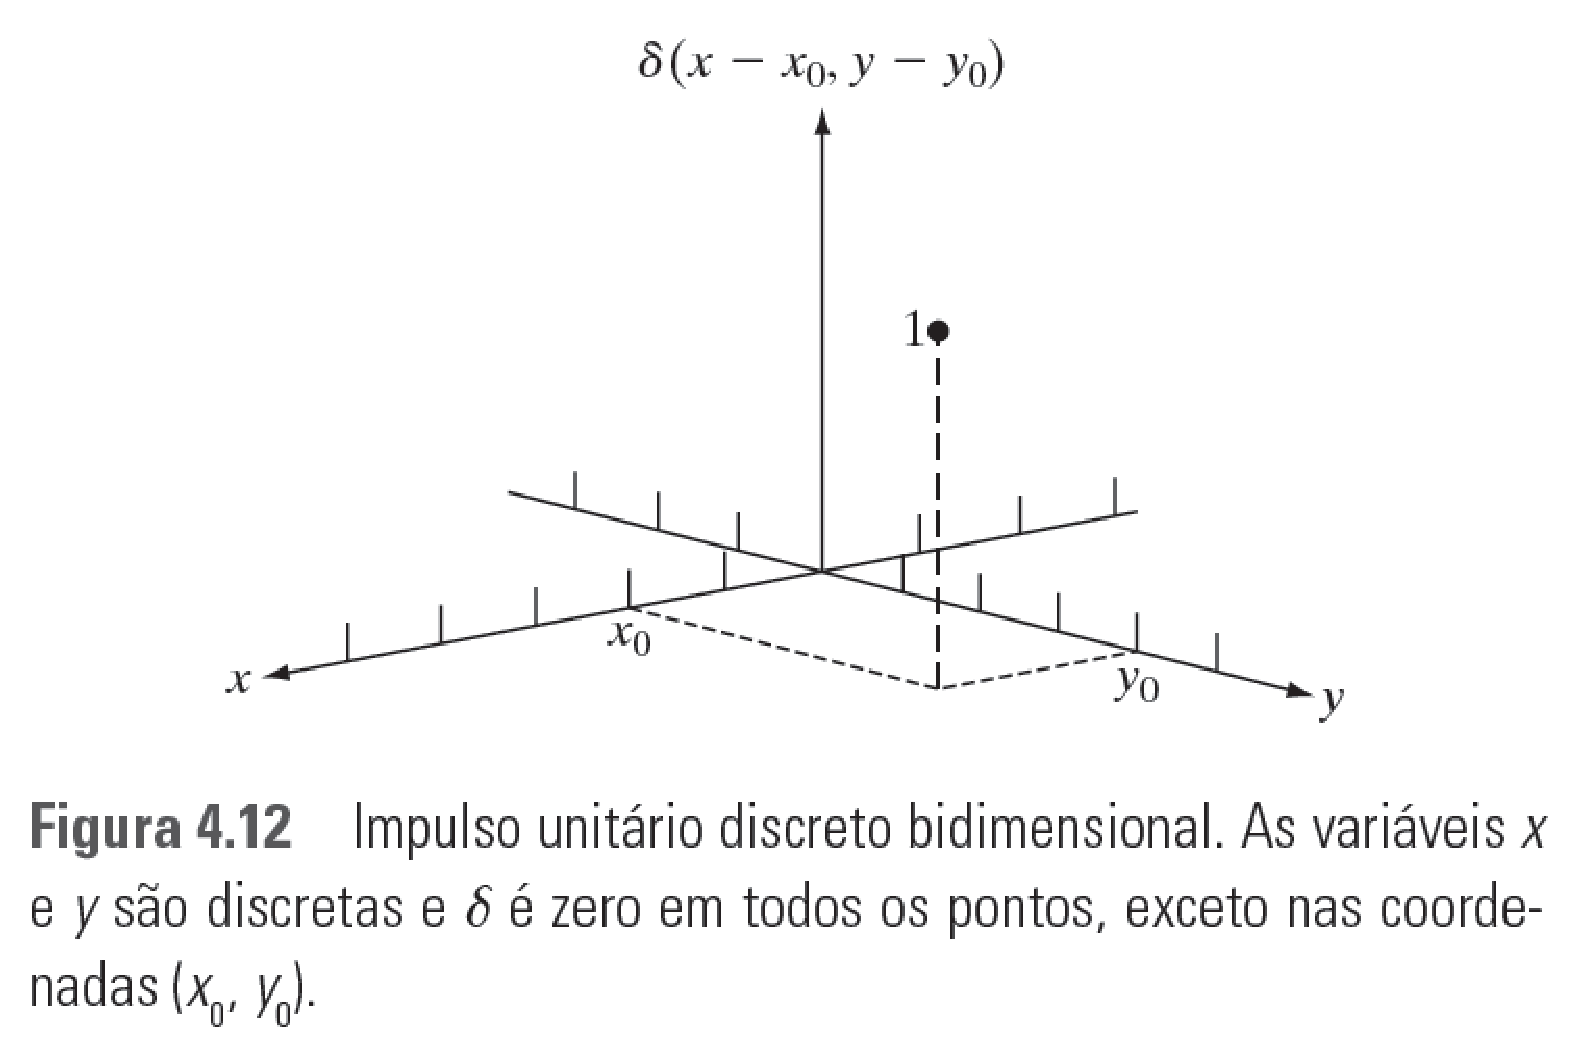
\includegraphics[width=0.55\textwidth]{figs/fig0412}
			 \end{center}
         \end{itemize}
      \end{slide}
      
      \begin{slide}[toc=]{Transformada de Fourier}
         \begin{itemize}[type=1]
            \item Análise
            \begin{equation*}
               F(u,v) = \sum_y\sum_x f(x,y) e^{-j(ux+vy)}
            \end{equation*}
            \item Síntese
            \begin{equation*}
               f(x,y) = \frac{1}{(2\pi)^2}\int_v\int_u F(u,v) e^{j(ux+vy)}du dv
            \end{equation*}
            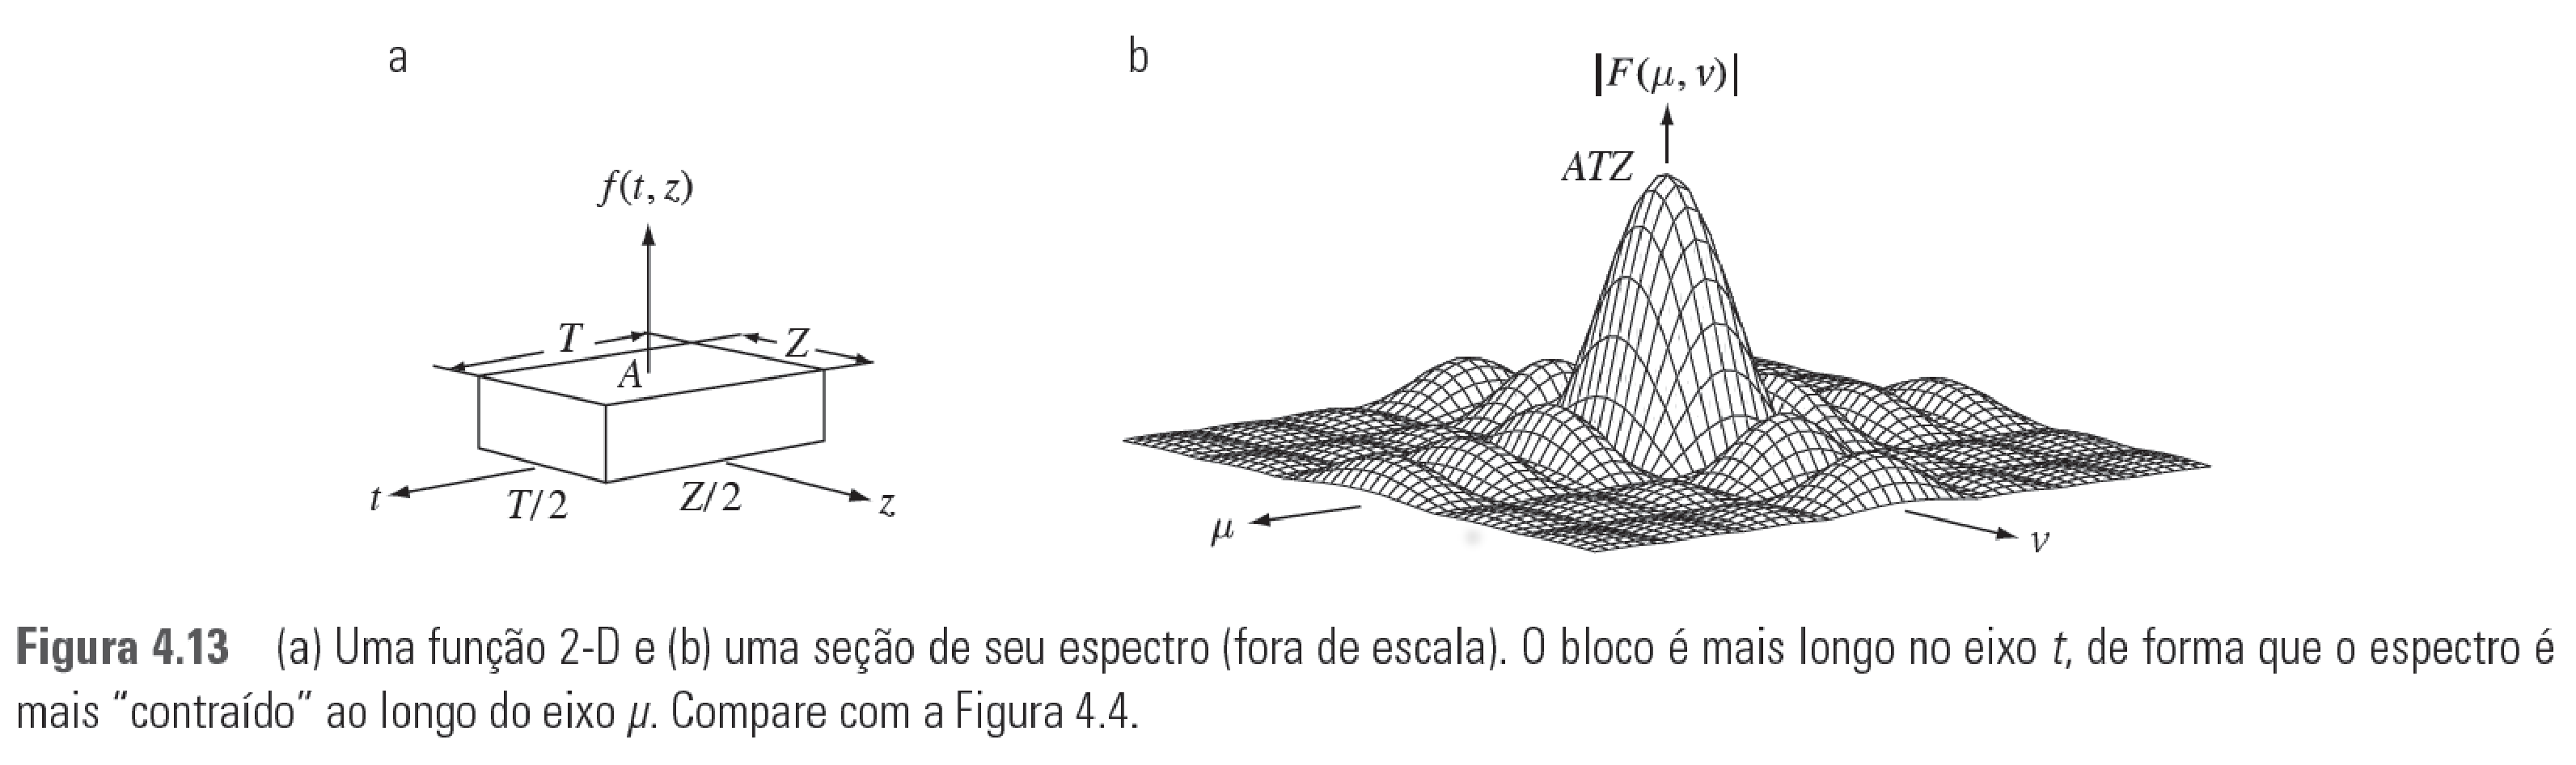
\includegraphics[width=0.95\textwidth]{figs/fig0413}
         \end{itemize}
      \end{slide}
      
      \begin{slide}[toc=]{Amostragem}
         \begin{itemize}[type=1]
            \item Todos os elementos da amostragem 1D são válidos:
            \begin{itemize}
               \item Sinal dever ser limitado em banda:
               \begin{equation*}
                  F(\mu,\nu) = 0 \text{ para } |\mu|\geq \mu_\text{max}, |\nu|\geq \nu_\text{max} 
               \end{equation*}
               \item Frequência de amostragem:
               \begin{equation*}
                  f_{st} \geq 2 \mu_\text{max}, f_{sz} \geq 2 \nu_\text{max}
               \end{equation*}
               \item Em geral, há necessidade de usar um filtro anti-aliasing
            \end{itemize}
         \end{itemize}
      \end{slide}
      
      \begin{slide}[toc=]{Amostragem}
         \begin{itemize}[type=1]
            \item Espectro resultante
         \end{itemize}
	      \begin{center}
		      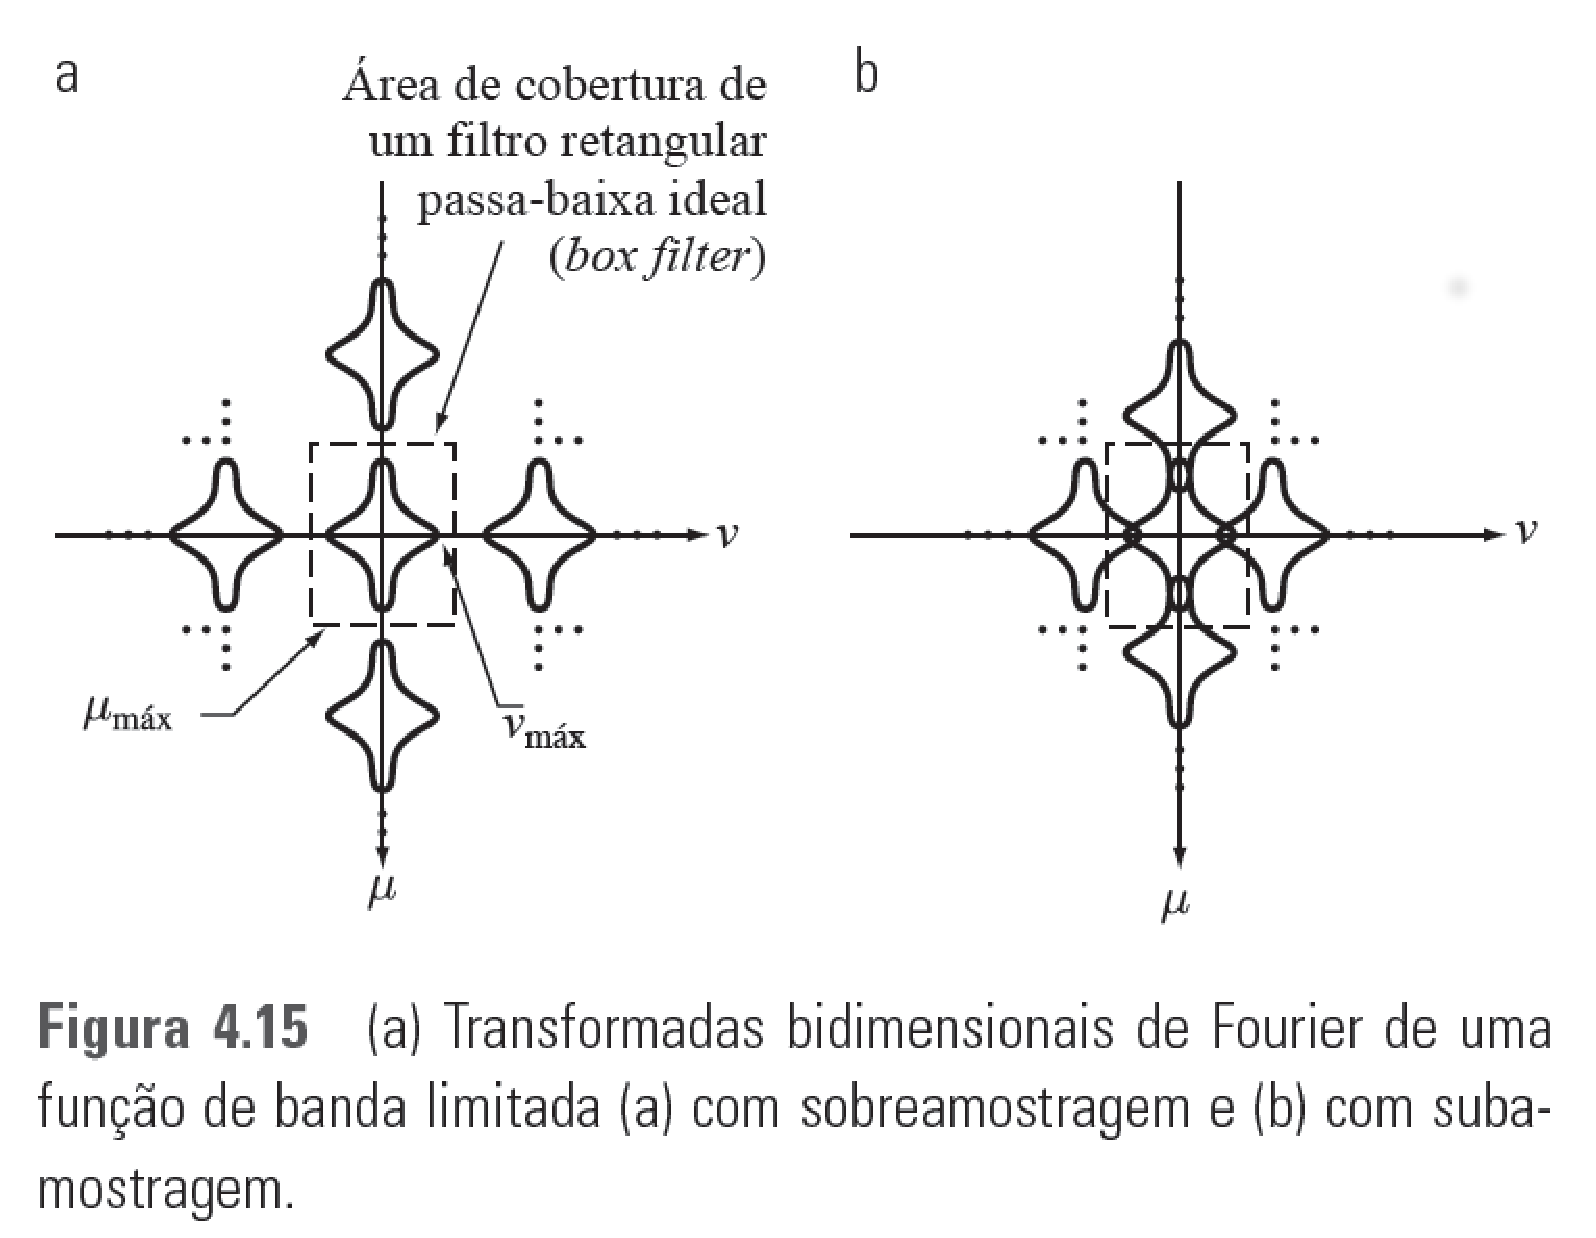
\includegraphics[width=0.60\textwidth]{figs/fig0415}
	      \end{center}
      \end{slide}

      \begin{slide}[toc=]{Amostragem}
         \begin{itemize}[type=1]
            \item Aliasing no domínio espacial
               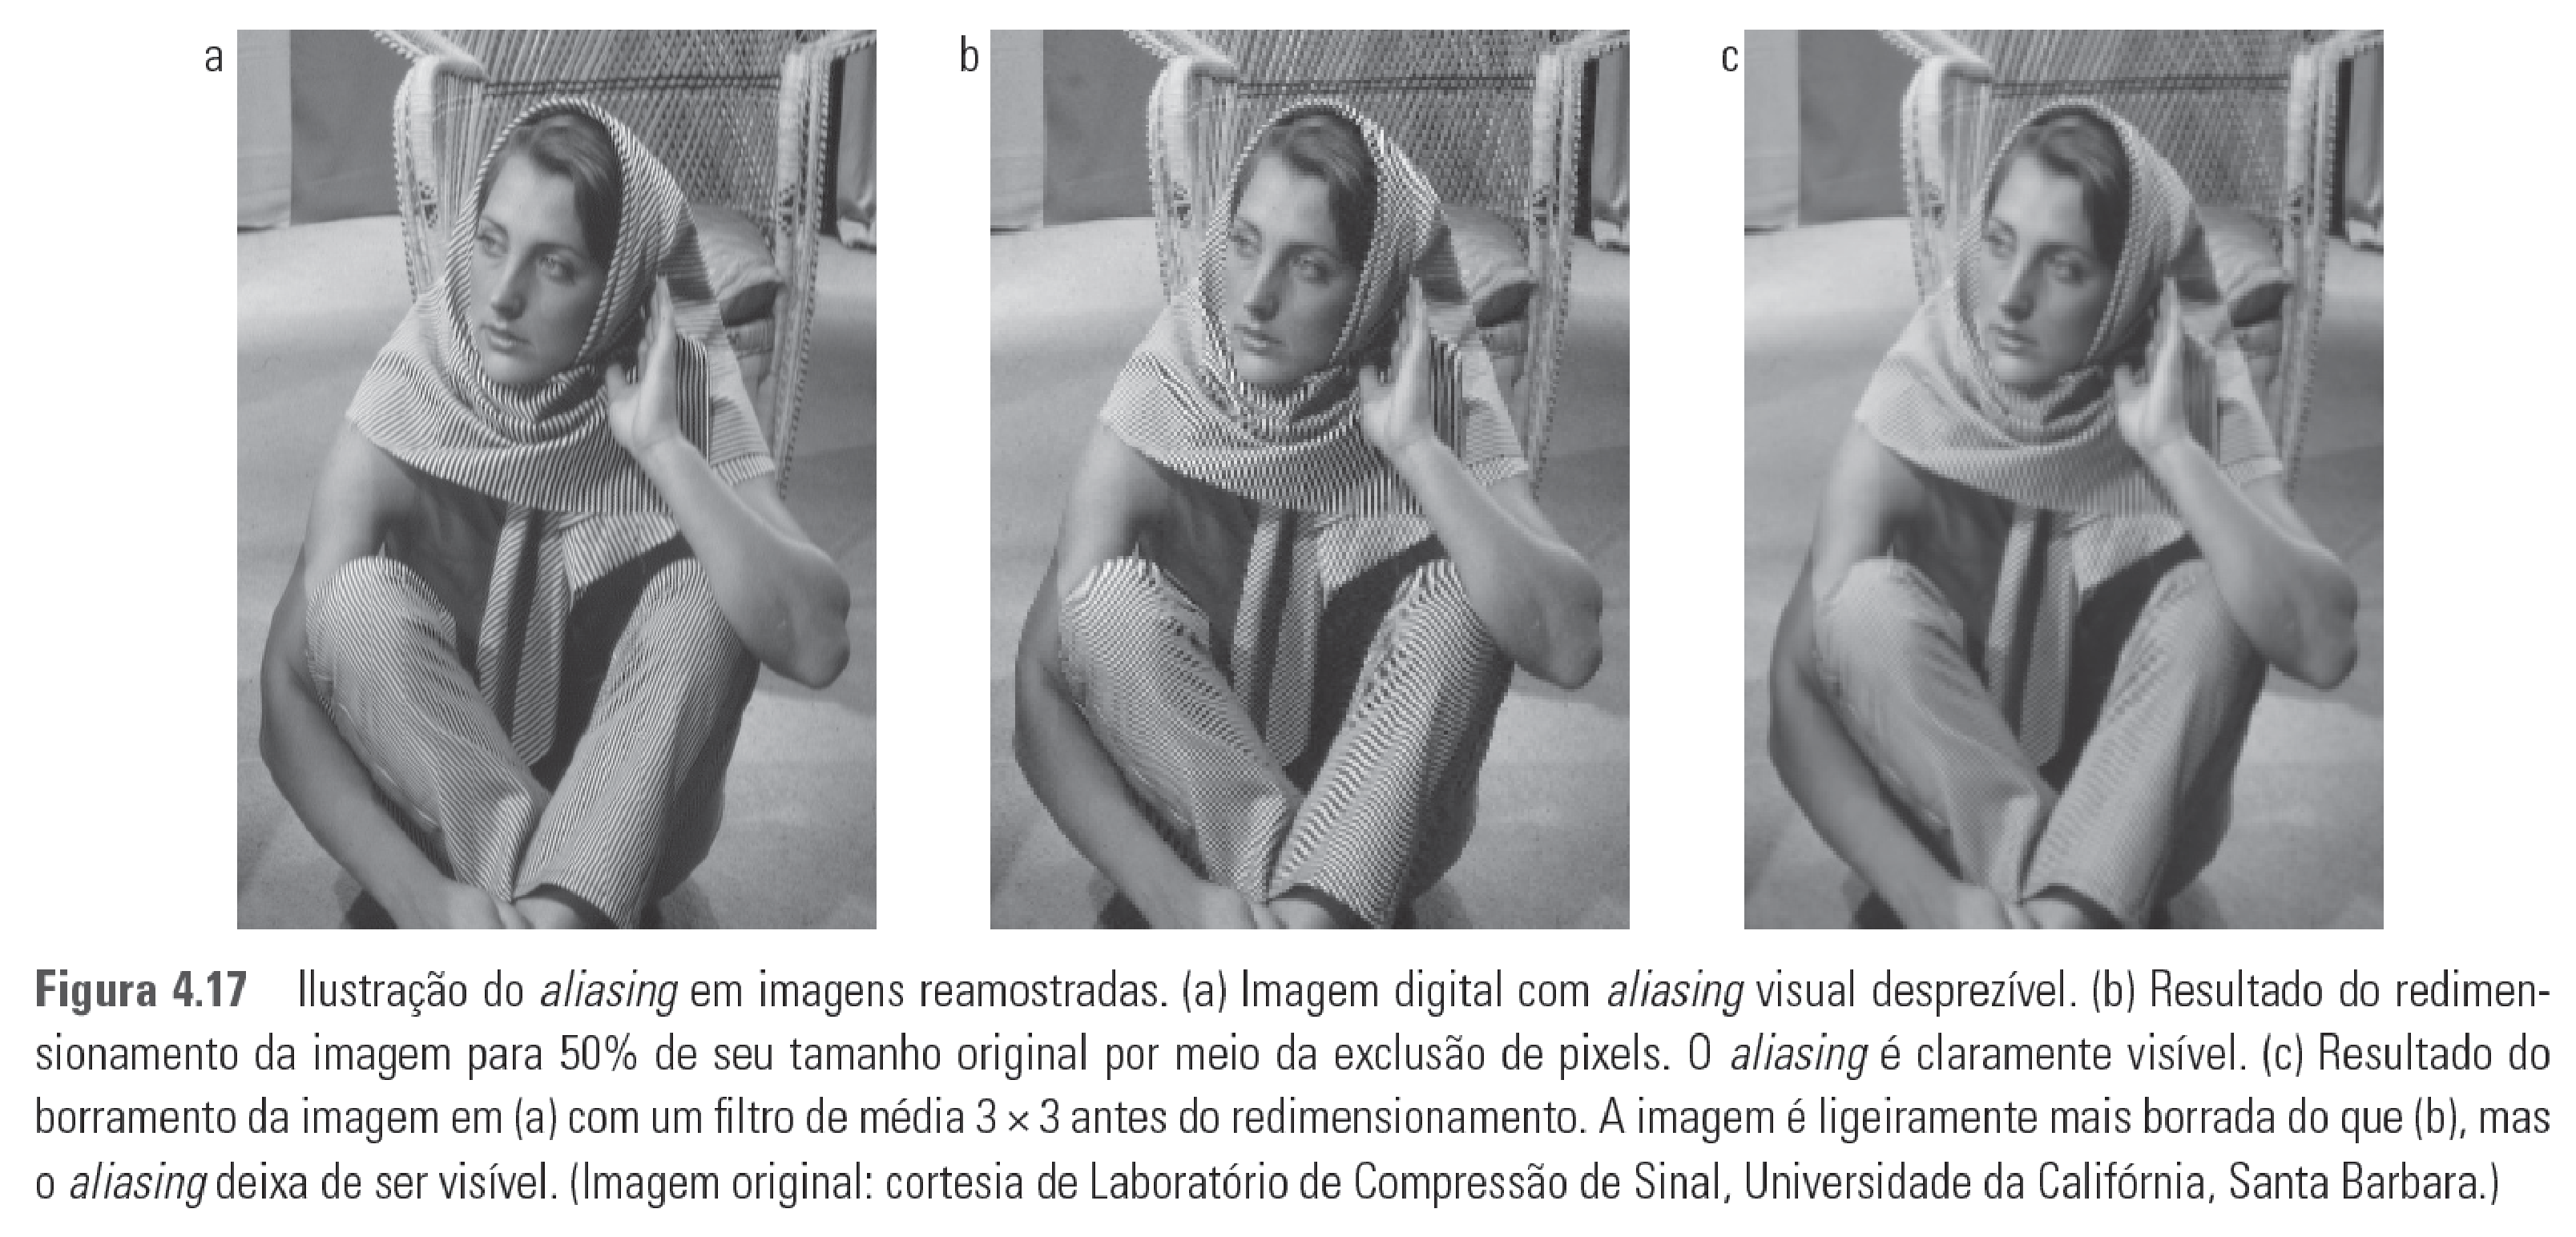
\includegraphics[width=\textwidth]{figs/fig0417}
         \end{itemize}
      \end{slide}
      
      \begin{slide}[toc=]{Exemplo de uma função simples}
         \begin{itemize}[type=1]
            \item Magnitude da Transformada de Fourier
         \end{itemize}
	      \begin{center}
               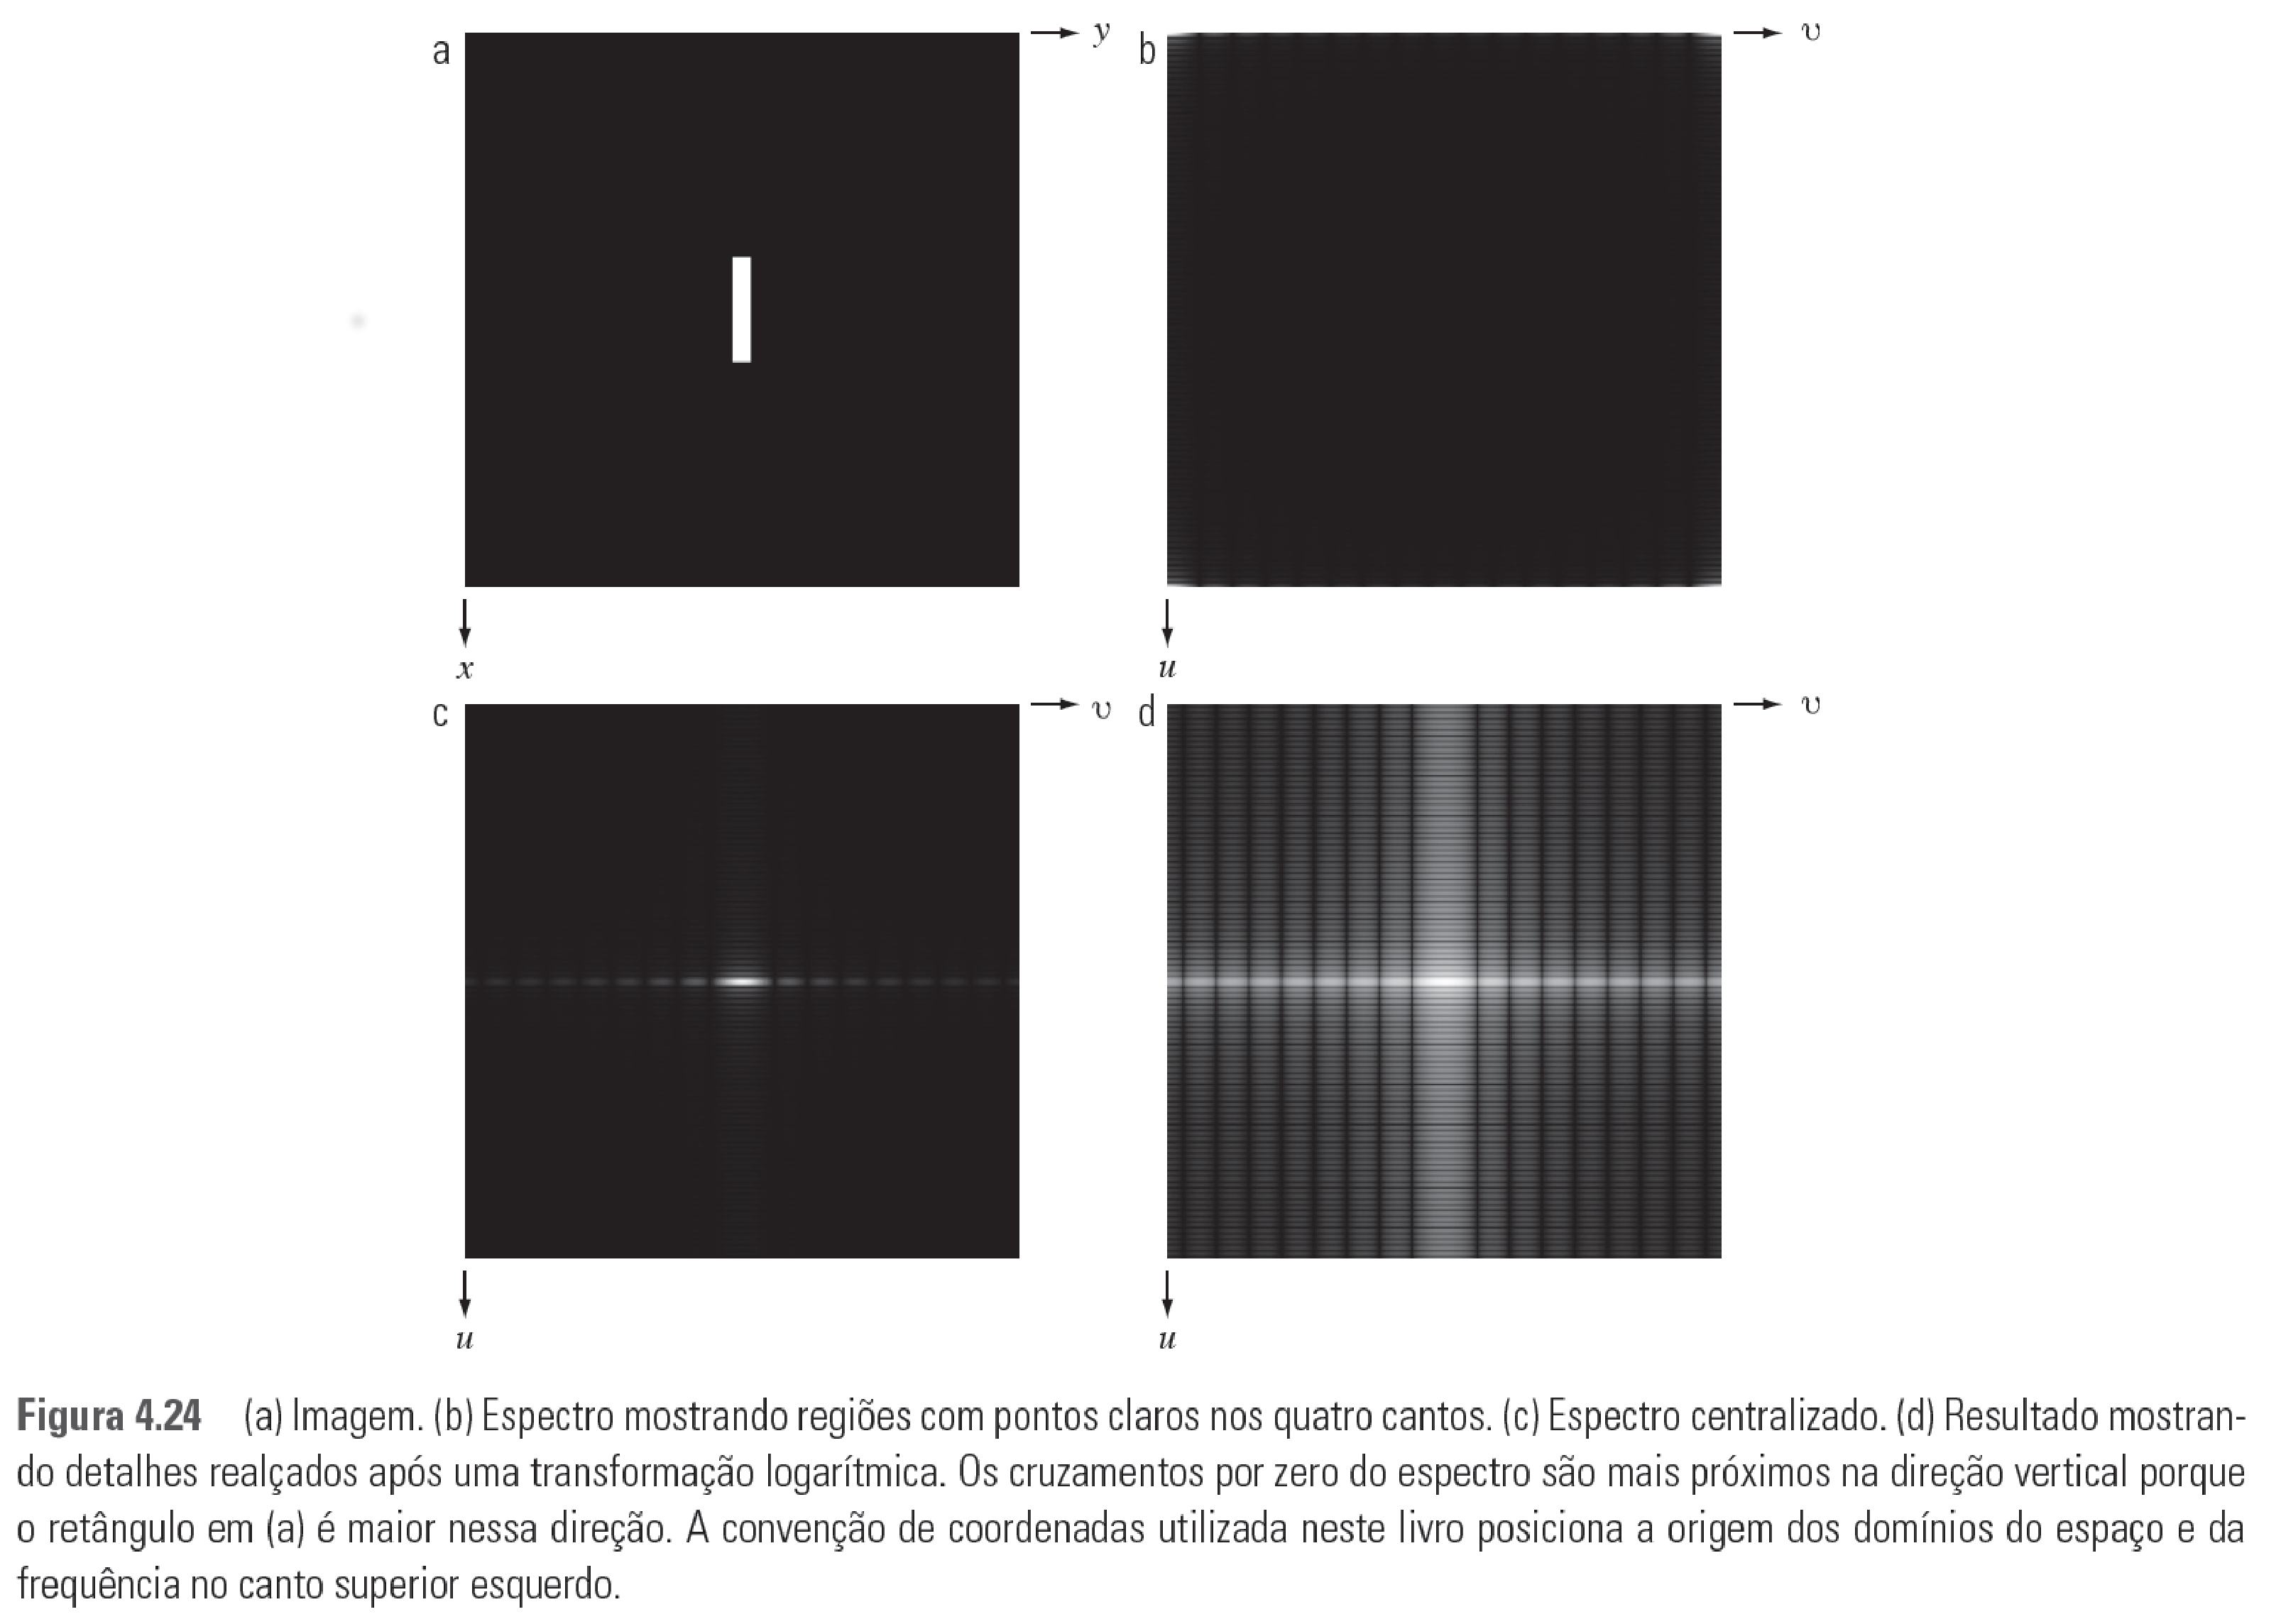
\includegraphics[width=0.65\textwidth]{figs/fig0424}
	      \end{center}
      \end{slide}
      
      \begin{slide}[toc=]{Efeitos do deslocamento e da rotação}
         \begin{itemize}[type=1]
            \item Magnitude da Transformada de Fourier
         \end{itemize}
	      \begin{center}
               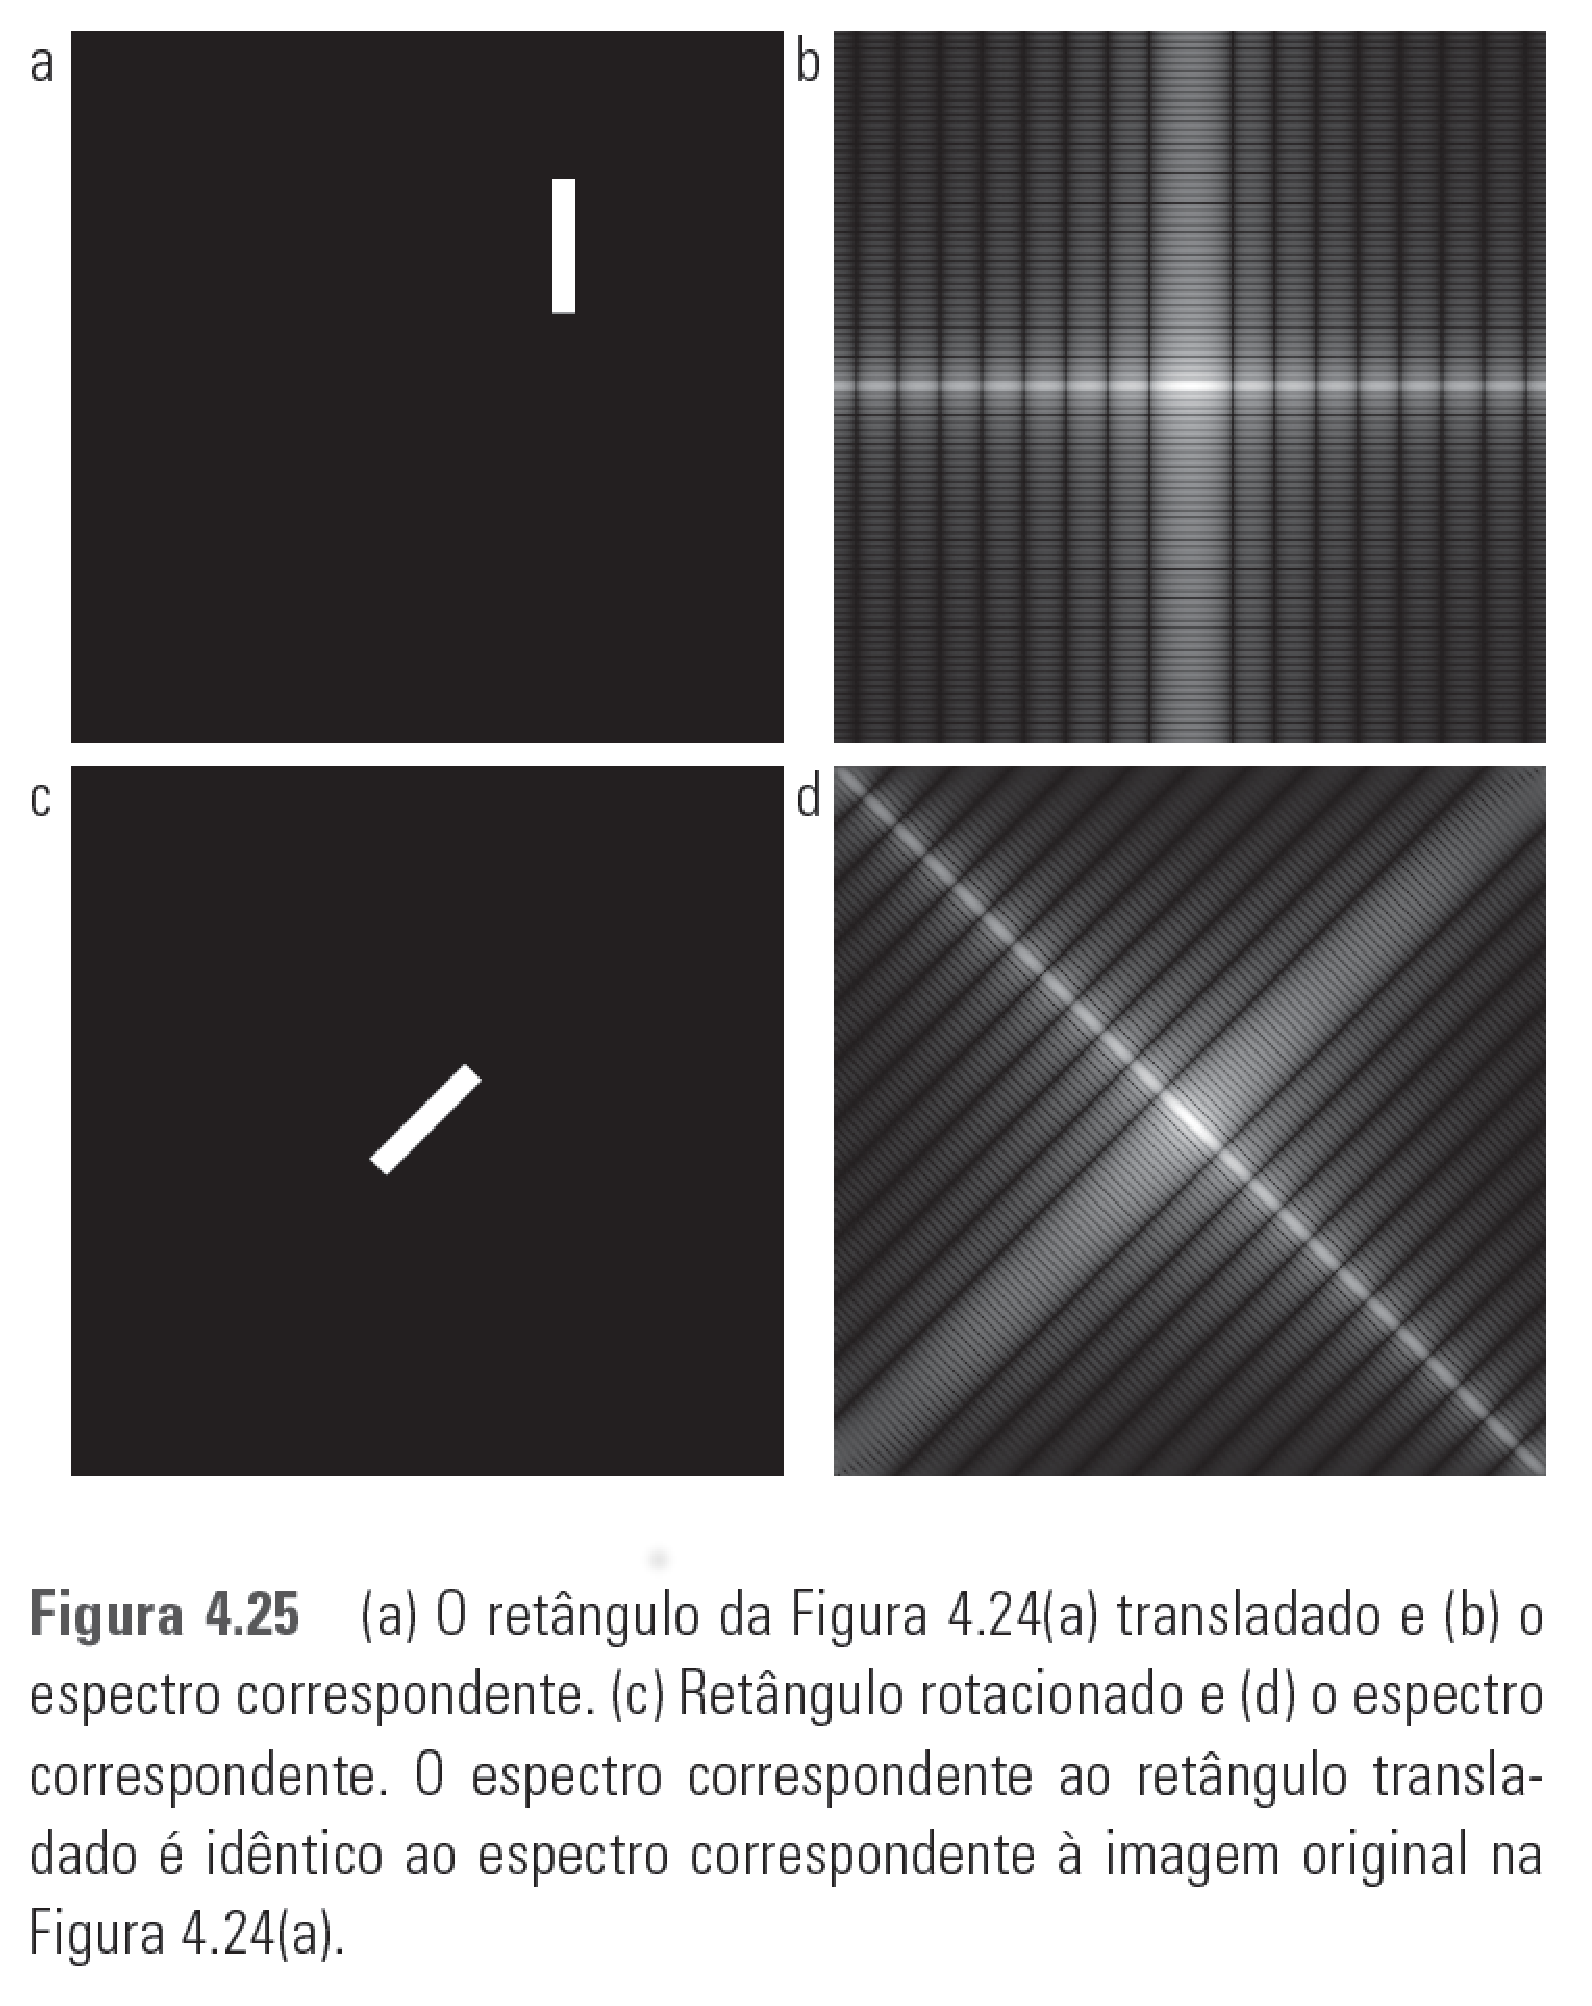
\includegraphics[width=0.35\textwidth]{figs/fig0425}
	      \end{center}
      \end{slide}
      
      \begin{slide}[toc=]{Informação visual na magnitude e fase}
         \begin{itemize}[type=1]
            \item Exemplo com imagem real
               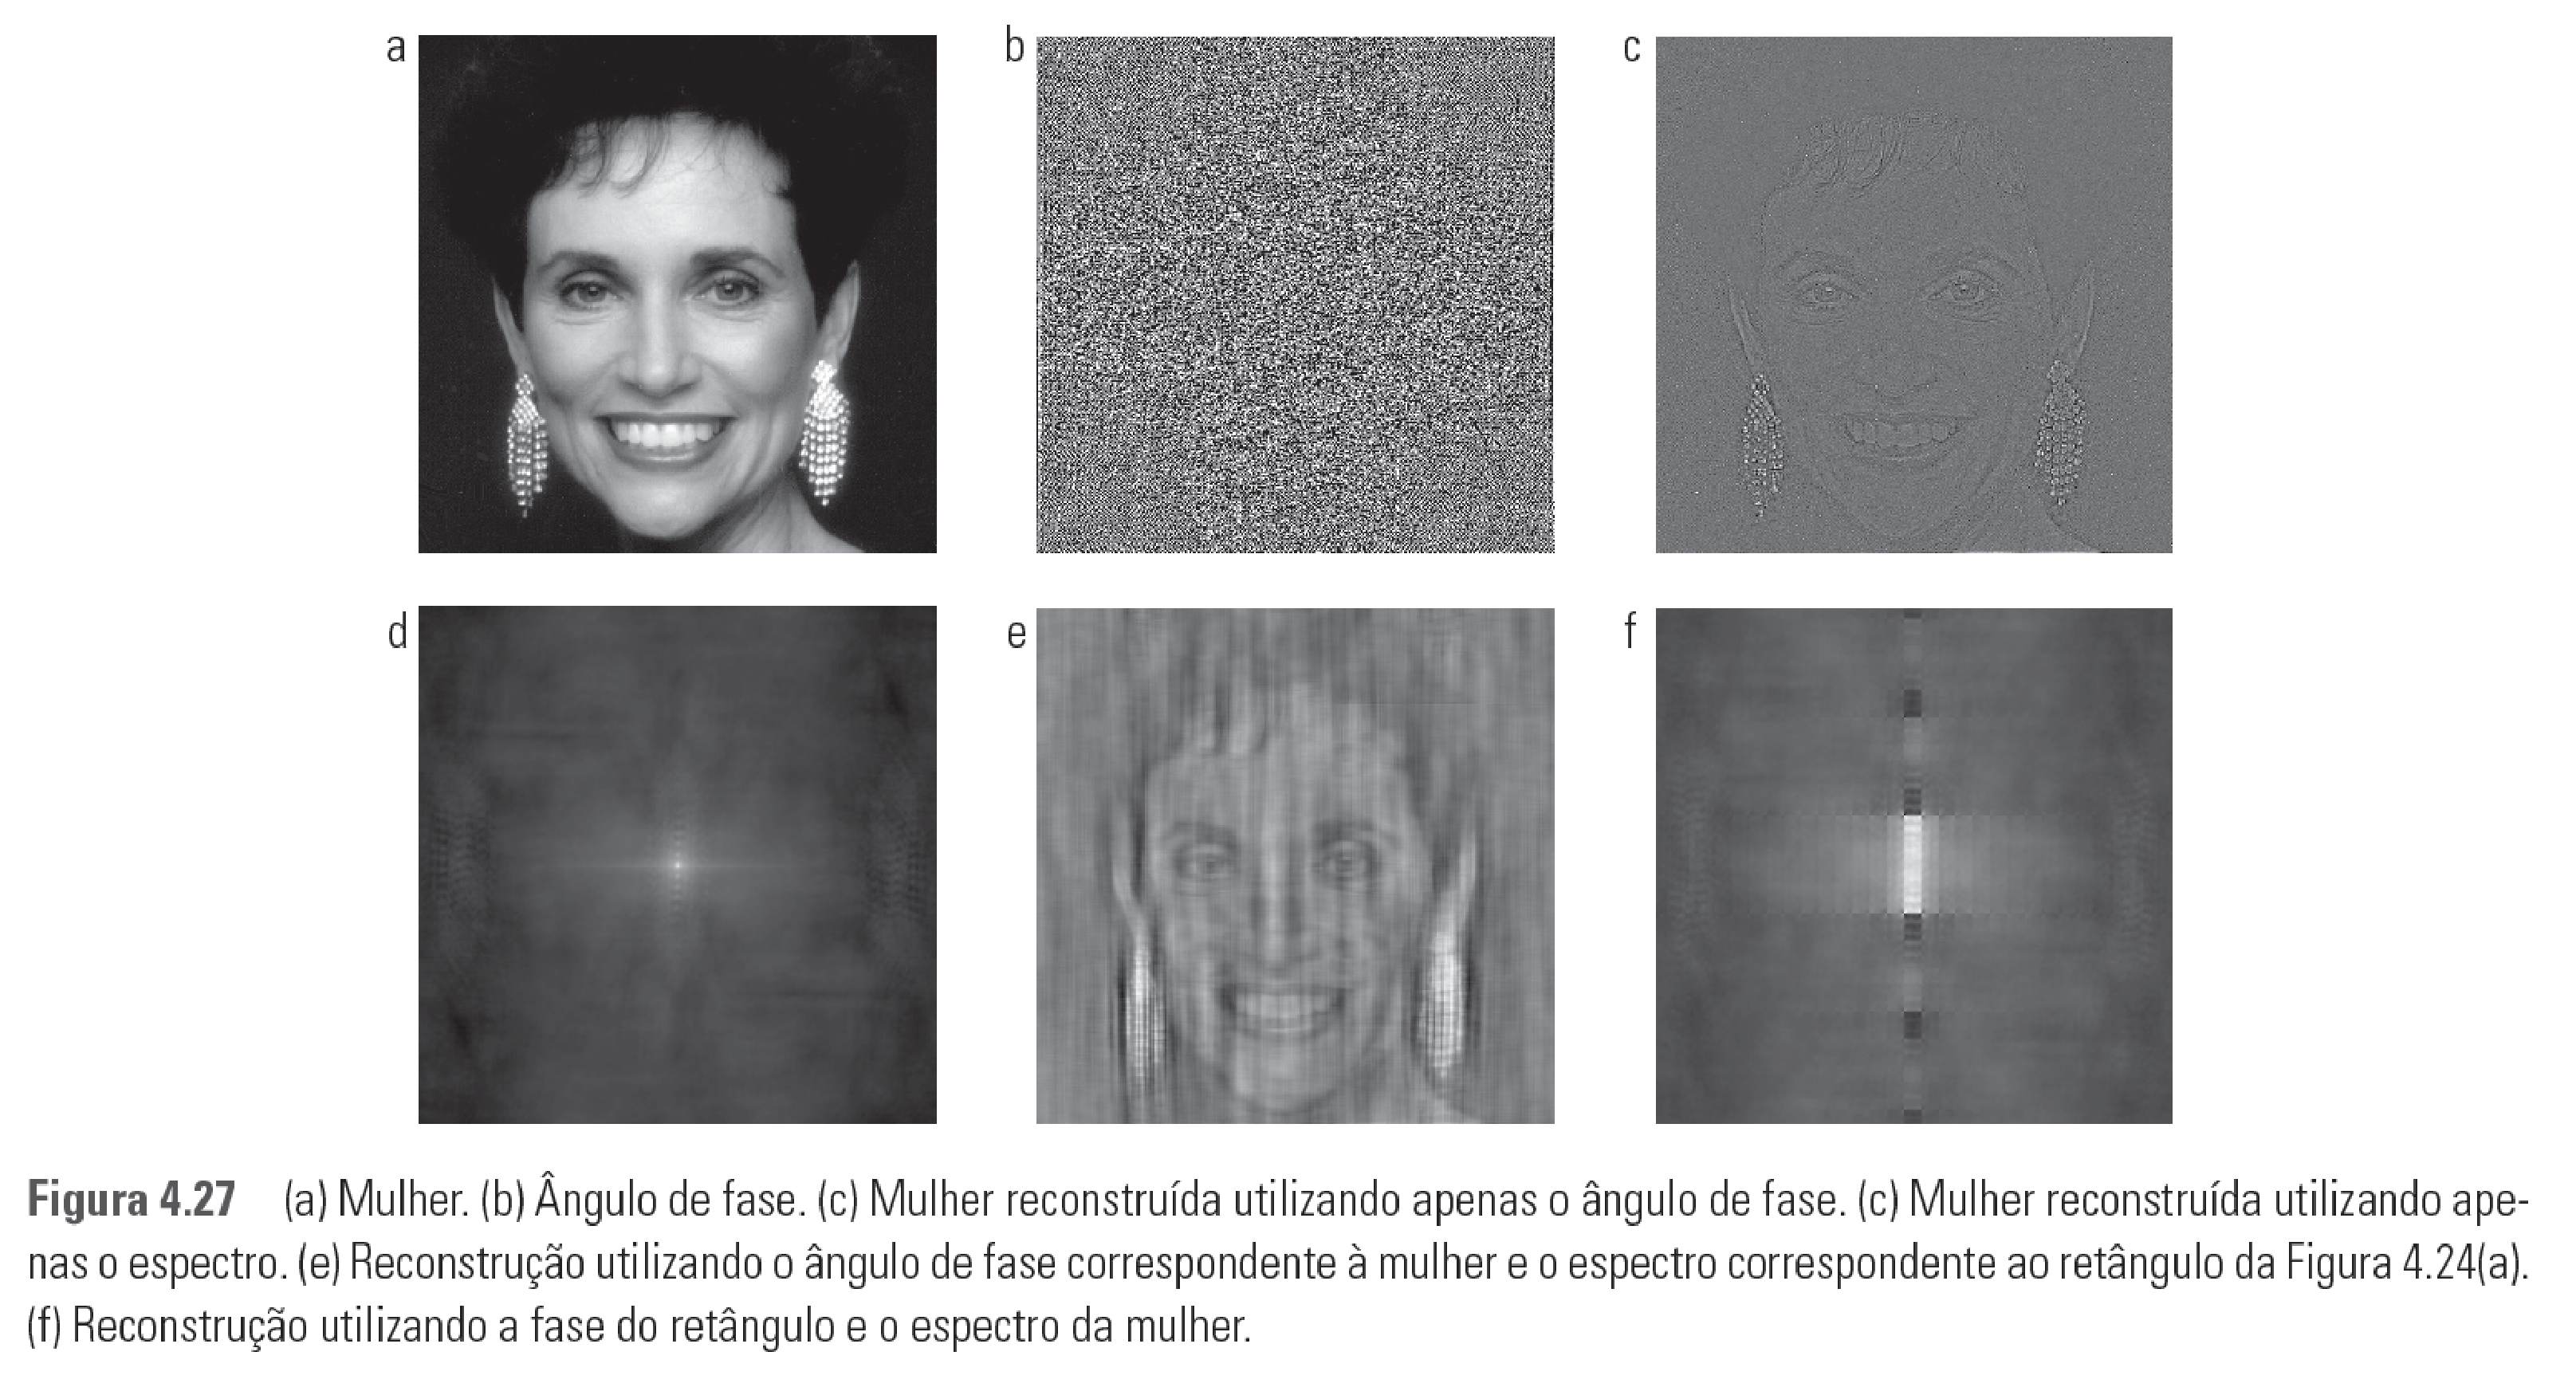
\includegraphics[width=0.95\textwidth]{figs/fig0427}
         \end{itemize}
      \end{slide}
      
      \begin{slide}[toc=]{Convolução 2D}
         \begin{itemize}[type=1]
            \item Domínio espacial
            \begin{equation*}
               g(x,y) = \sum_n\sum_m h(m,n)f(x-m,y-n)
            \end{equation*}
            \item Domínio transformado
            \begin{equation*}
               G(u,v) = H(u,v)F(u,v)
            \end{equation*}
         \end{itemize}
      \end{slide}
   
   \section[slide=true]{Fundamentos da filtragem no domínio da frequência}
      \begin{slide}[toc=]{Relação entre domínios}
         \begin{itemize}[type=1]
            \item Decomposição da imagem em componenentes espectrais em diferentes direções
            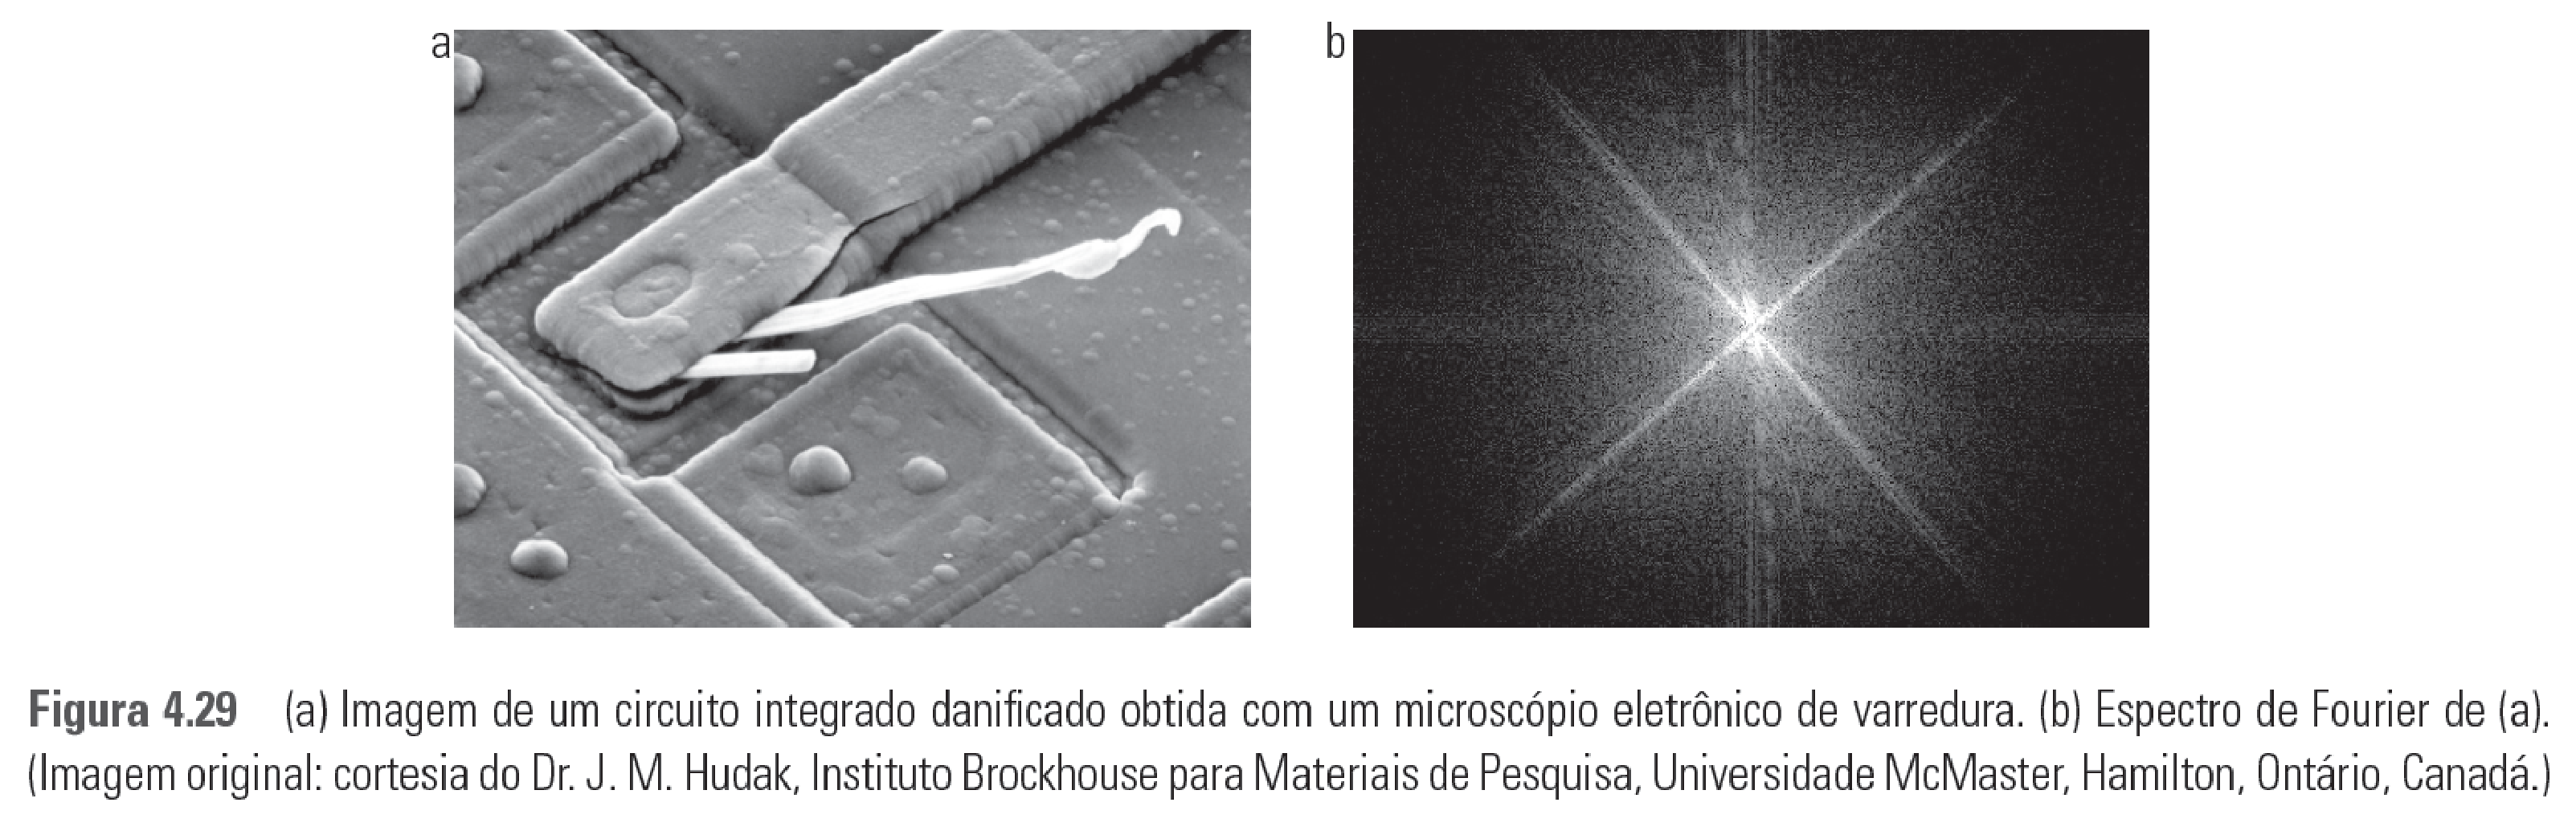
\includegraphics[width=0.9\textwidth]{figs/fig0429}
            \item Procedimento básico:
            \begin{equation*}
               g(x,y) = \text{IFFT}[H(u,v)F(u,v)]
            \end{equation*}
            $H(u,v)$: reposta em frequência do filtro\\
            $F(u,v)$: FFT de da imagem de entrada $f(x,y)$\\
            $g(x,y)$: imagem resultante (domínio espacial)
         \end{itemize}
      \end{slide}
      
      \begin{slide}[toc=]{Filtragem e seus efeitos}
         \begin{itemize}[type=1]
            \item Filtros diversos
         \end{itemize}
	      \begin{center}
            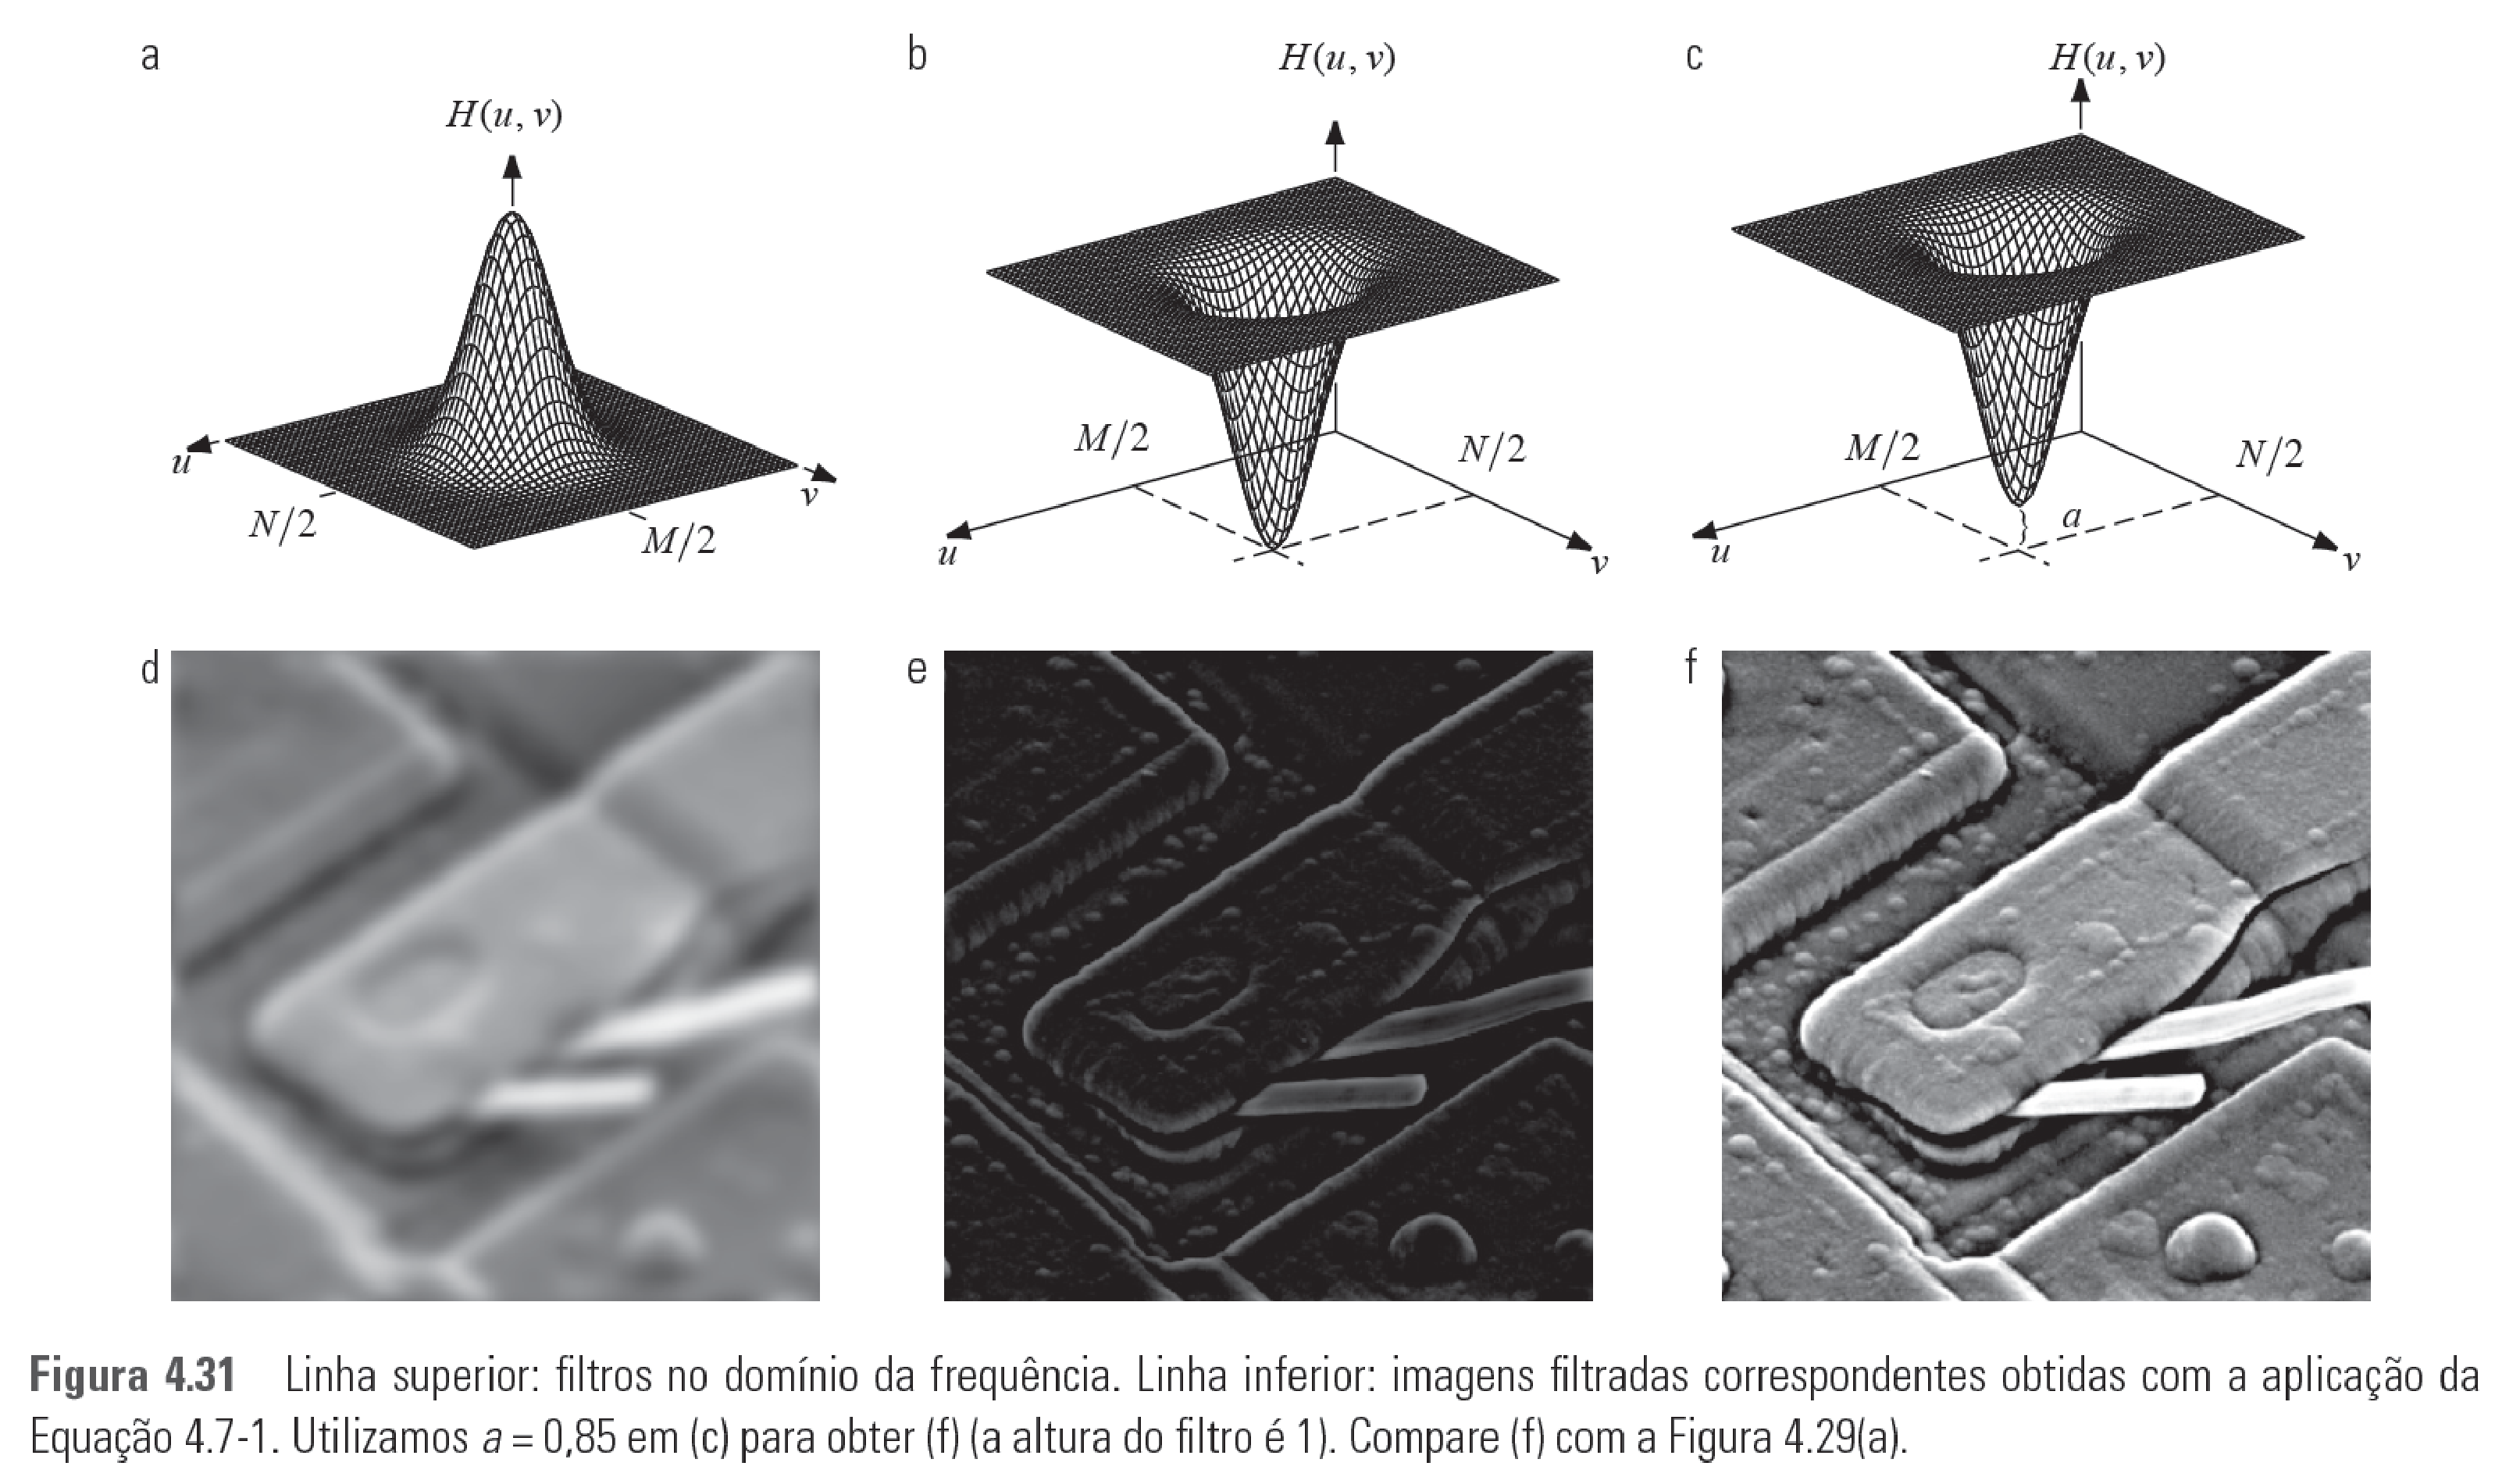
\includegraphics[width=0.75\textwidth]{figs/fig0431}
	      \end{center}
      \end{slide}
      
      \begin{slide}[toc=]{Observações sobre a FFT}
         \begin{itemize}[type=1]
            \item Cuidado com as dimensões dos sinais ($L_g = L_f+L_h -1$)
         \end{itemize}
	      \begin{center}
            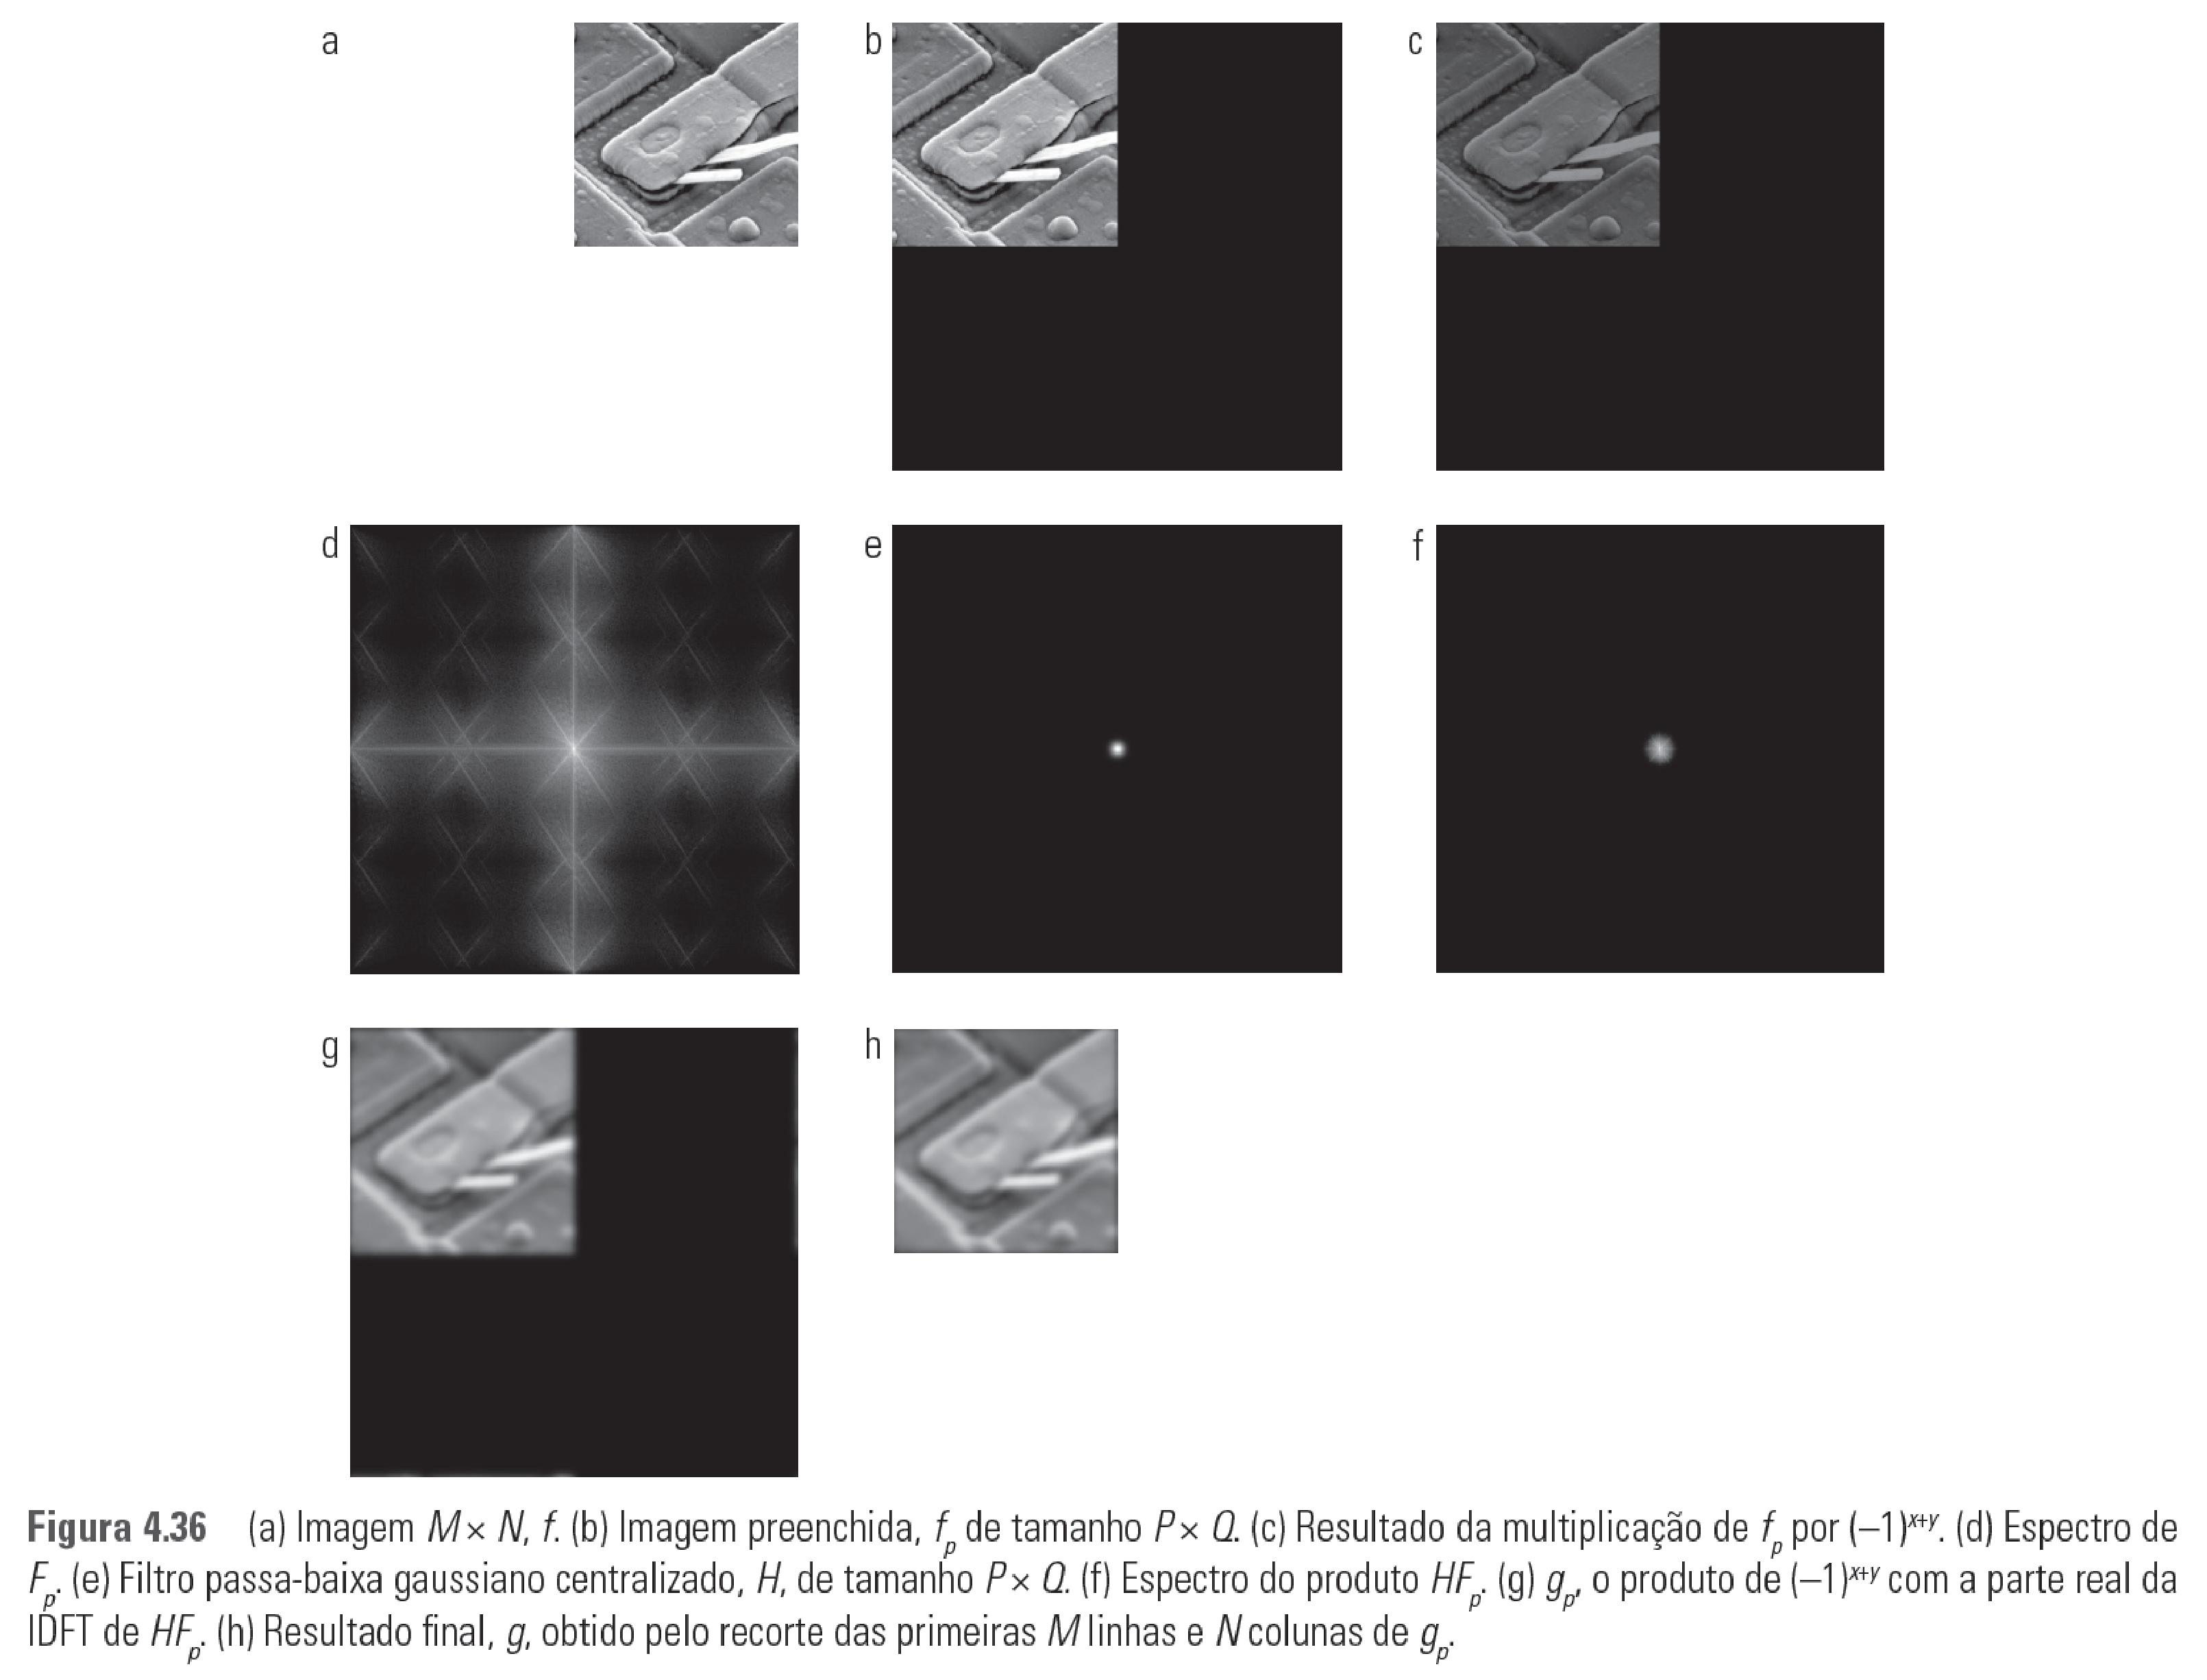
\includegraphics[width=0.9\textheight]{figs/fig0436}
	      \end{center}
      \end{slide}
      
   \section[slide=true]{Suavização de imagens}
      \begin{slide}[toc=]{Filtro passa baixa ideal}
         \begin{itemize}[type=1]
            \item Resposta em frequência
            \begin{equation*}
               H(u,v) = \begin{cases}
                           1& \text{se }D(u,v)\leq D_0\\
                           0& \text{se }D(u,v)> D_0
                        \end{cases}
            \end{equation*}
            $D(u,v)$: distância de um ponto $(u,v)$ à origem
            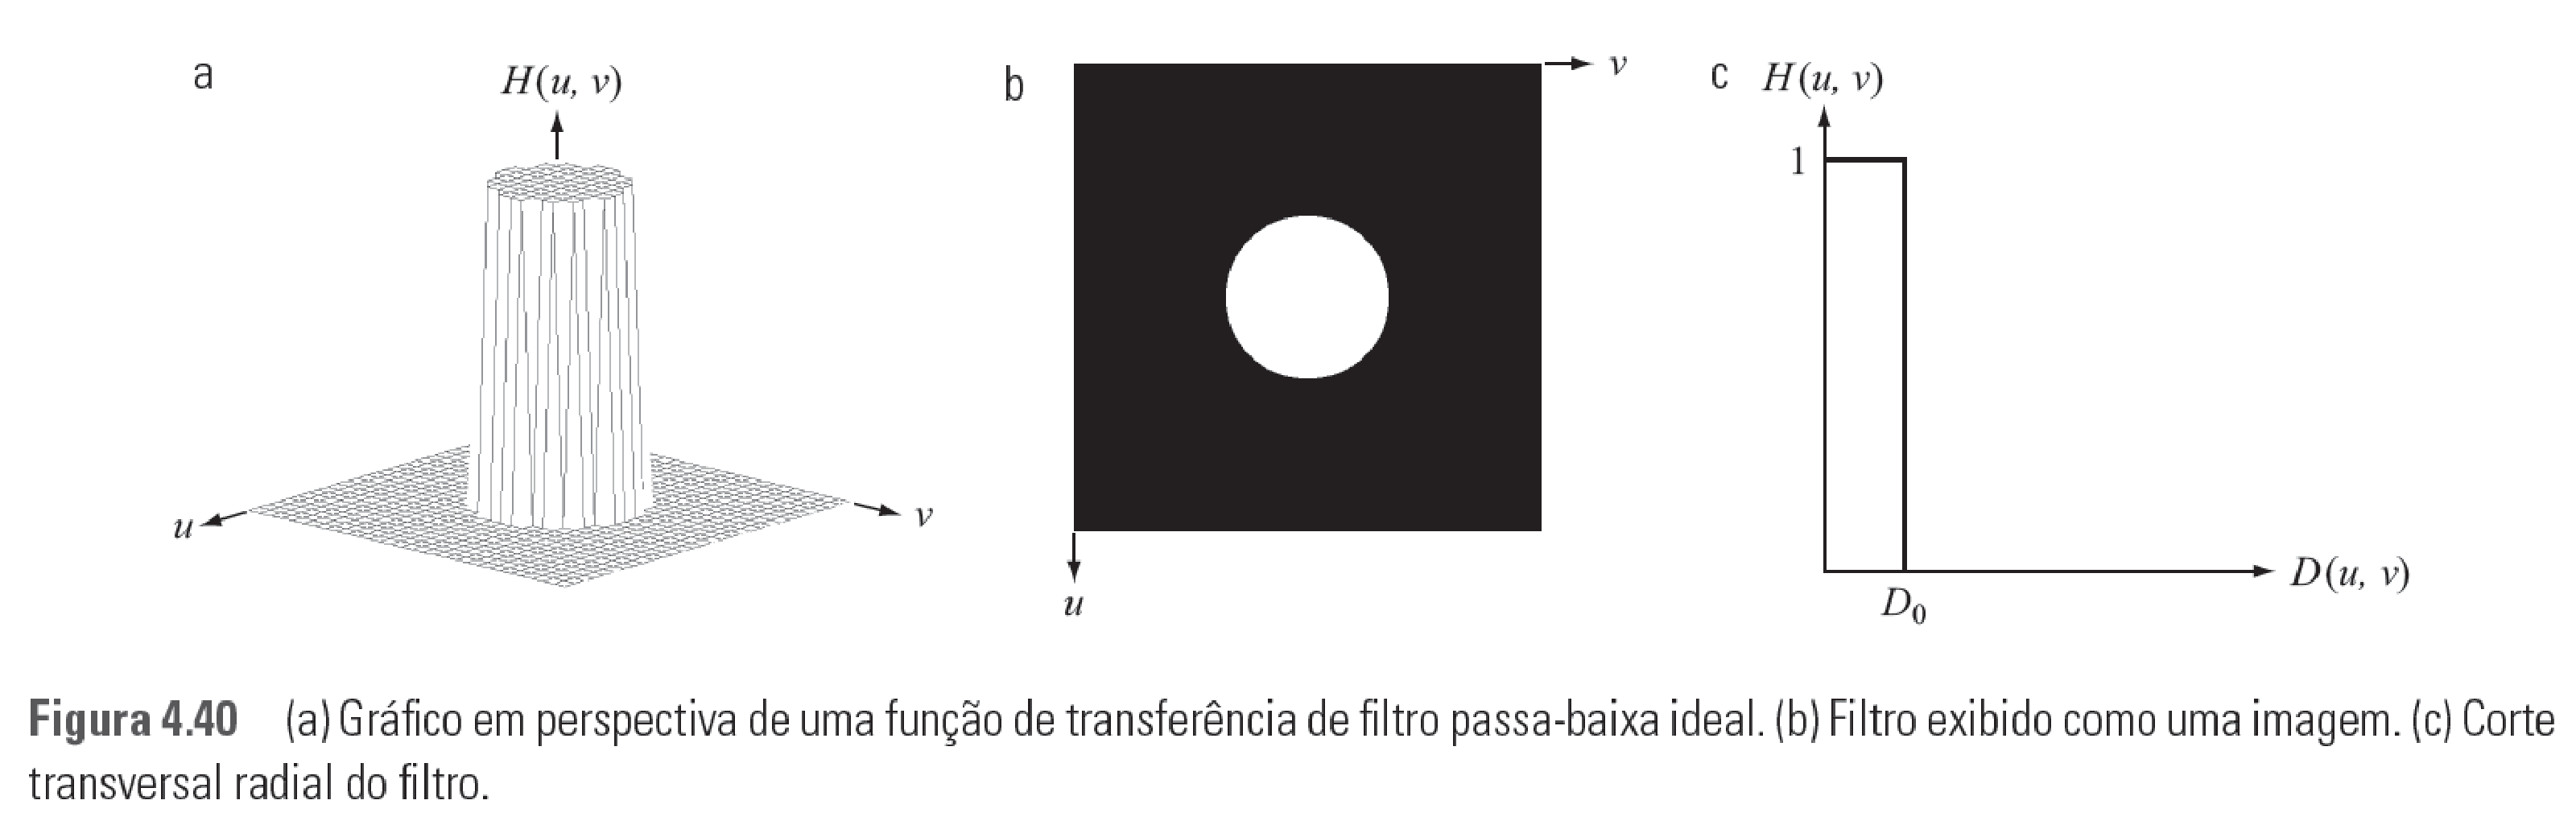
\includegraphics[width=0.95\textwidth]{figs/fig0440}
         \end{itemize}
      \end{slide}
      
      \begin{slide}[toc=]{Filtro passa baixa ideal}
         \begin{itemize}[type=1]
            \item Valor de $D_0$ em função do percentual de energia da imagem ($\alpha$)
            \begin{equation*}
               \alpha = 100 \sum_{(u,v)\in \Phi_{D_0}}{\frac{|F(u,v)|^2}{E_T}}
            \end{equation*}
            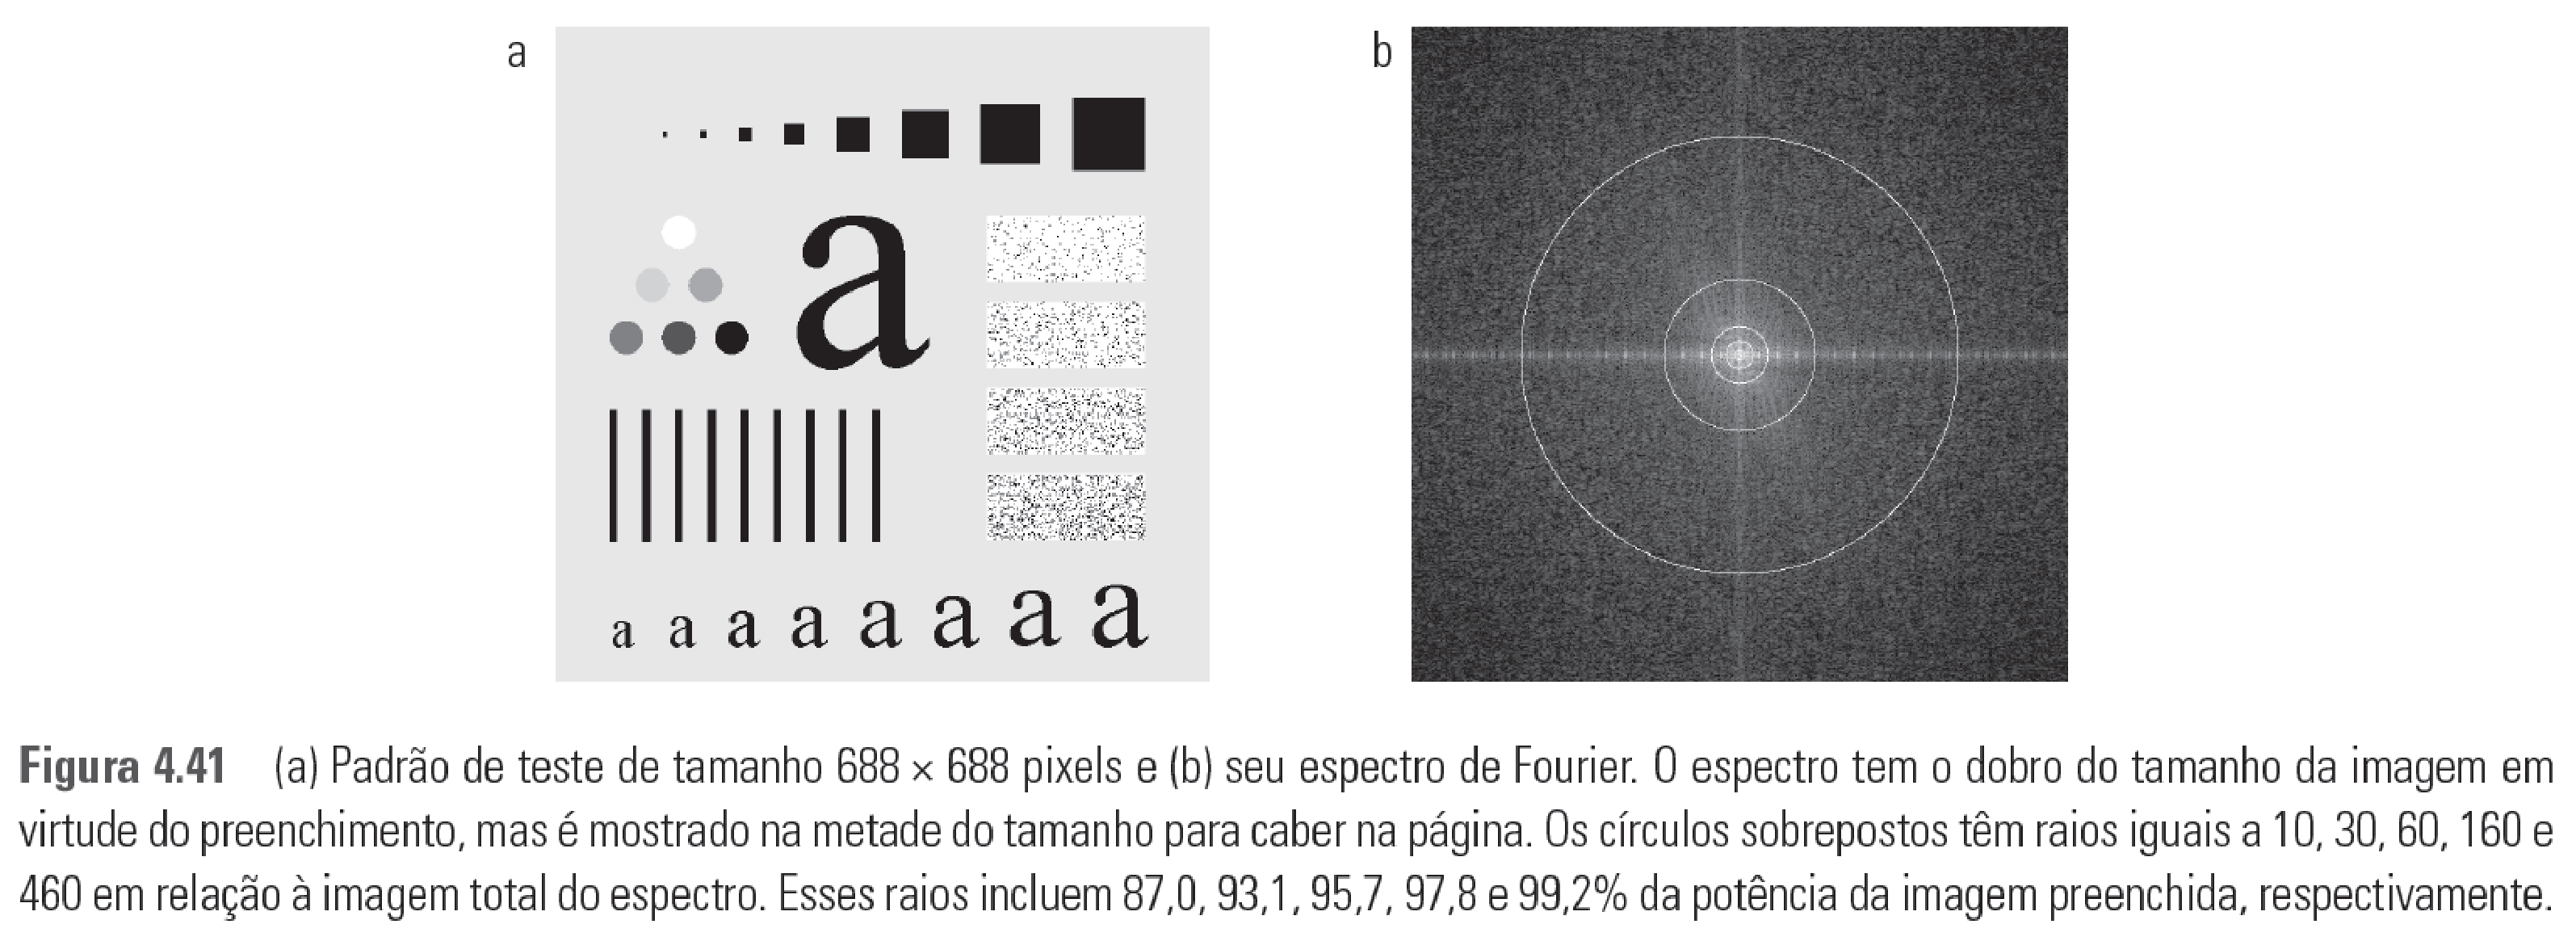
\includegraphics[width=0.95\textwidth]{figs/fig0441}
         \end{itemize}
      \end{slide}
      
      \begin{slide}[toc=]{Filtro passa baixa ideal}
         \begin{itemize}[type=1]
            \item Resultado para diferentes valores de $\alpha$
         \end{itemize}
	      \begin{center}
            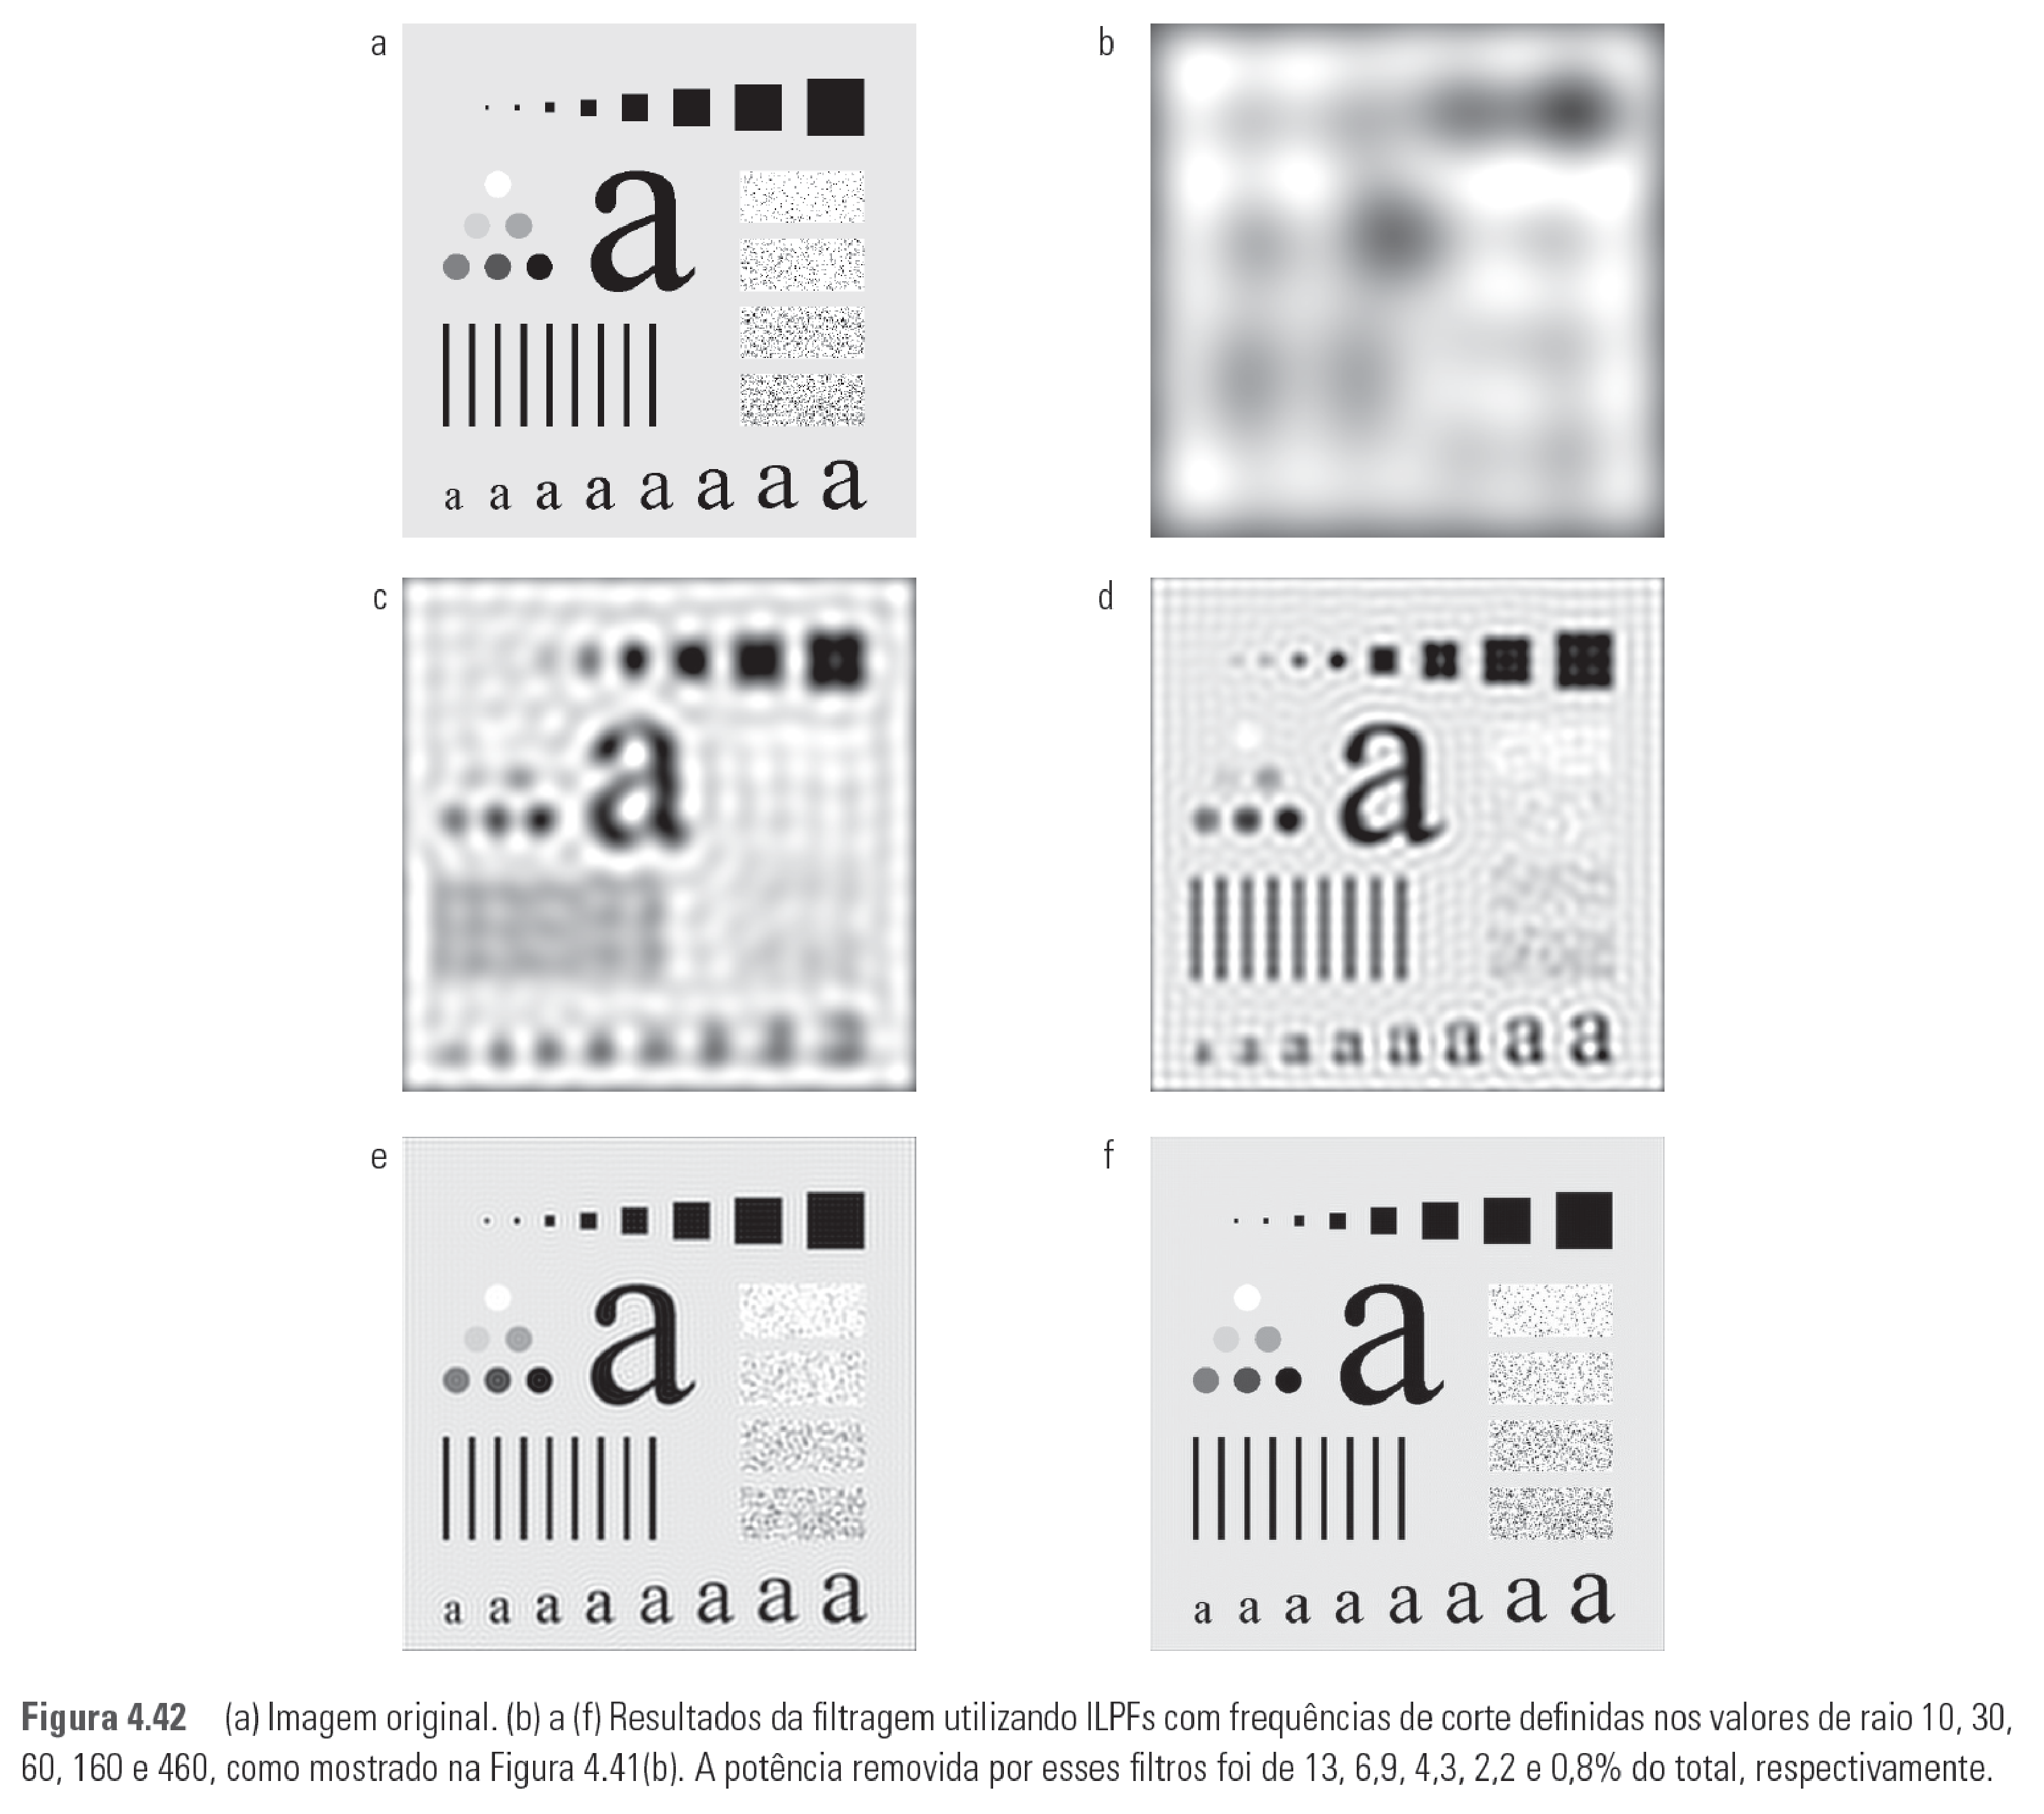
\includegraphics[height=0.7\textheight]{figs/fig0442}
	      \end{center}
      \end{slide}
      
      \begin{slide}[toc=]{Filtro passa baixa ideal}
         \begin{itemize}[type=1]
            \item Efeitos de anelamento (ringing)
            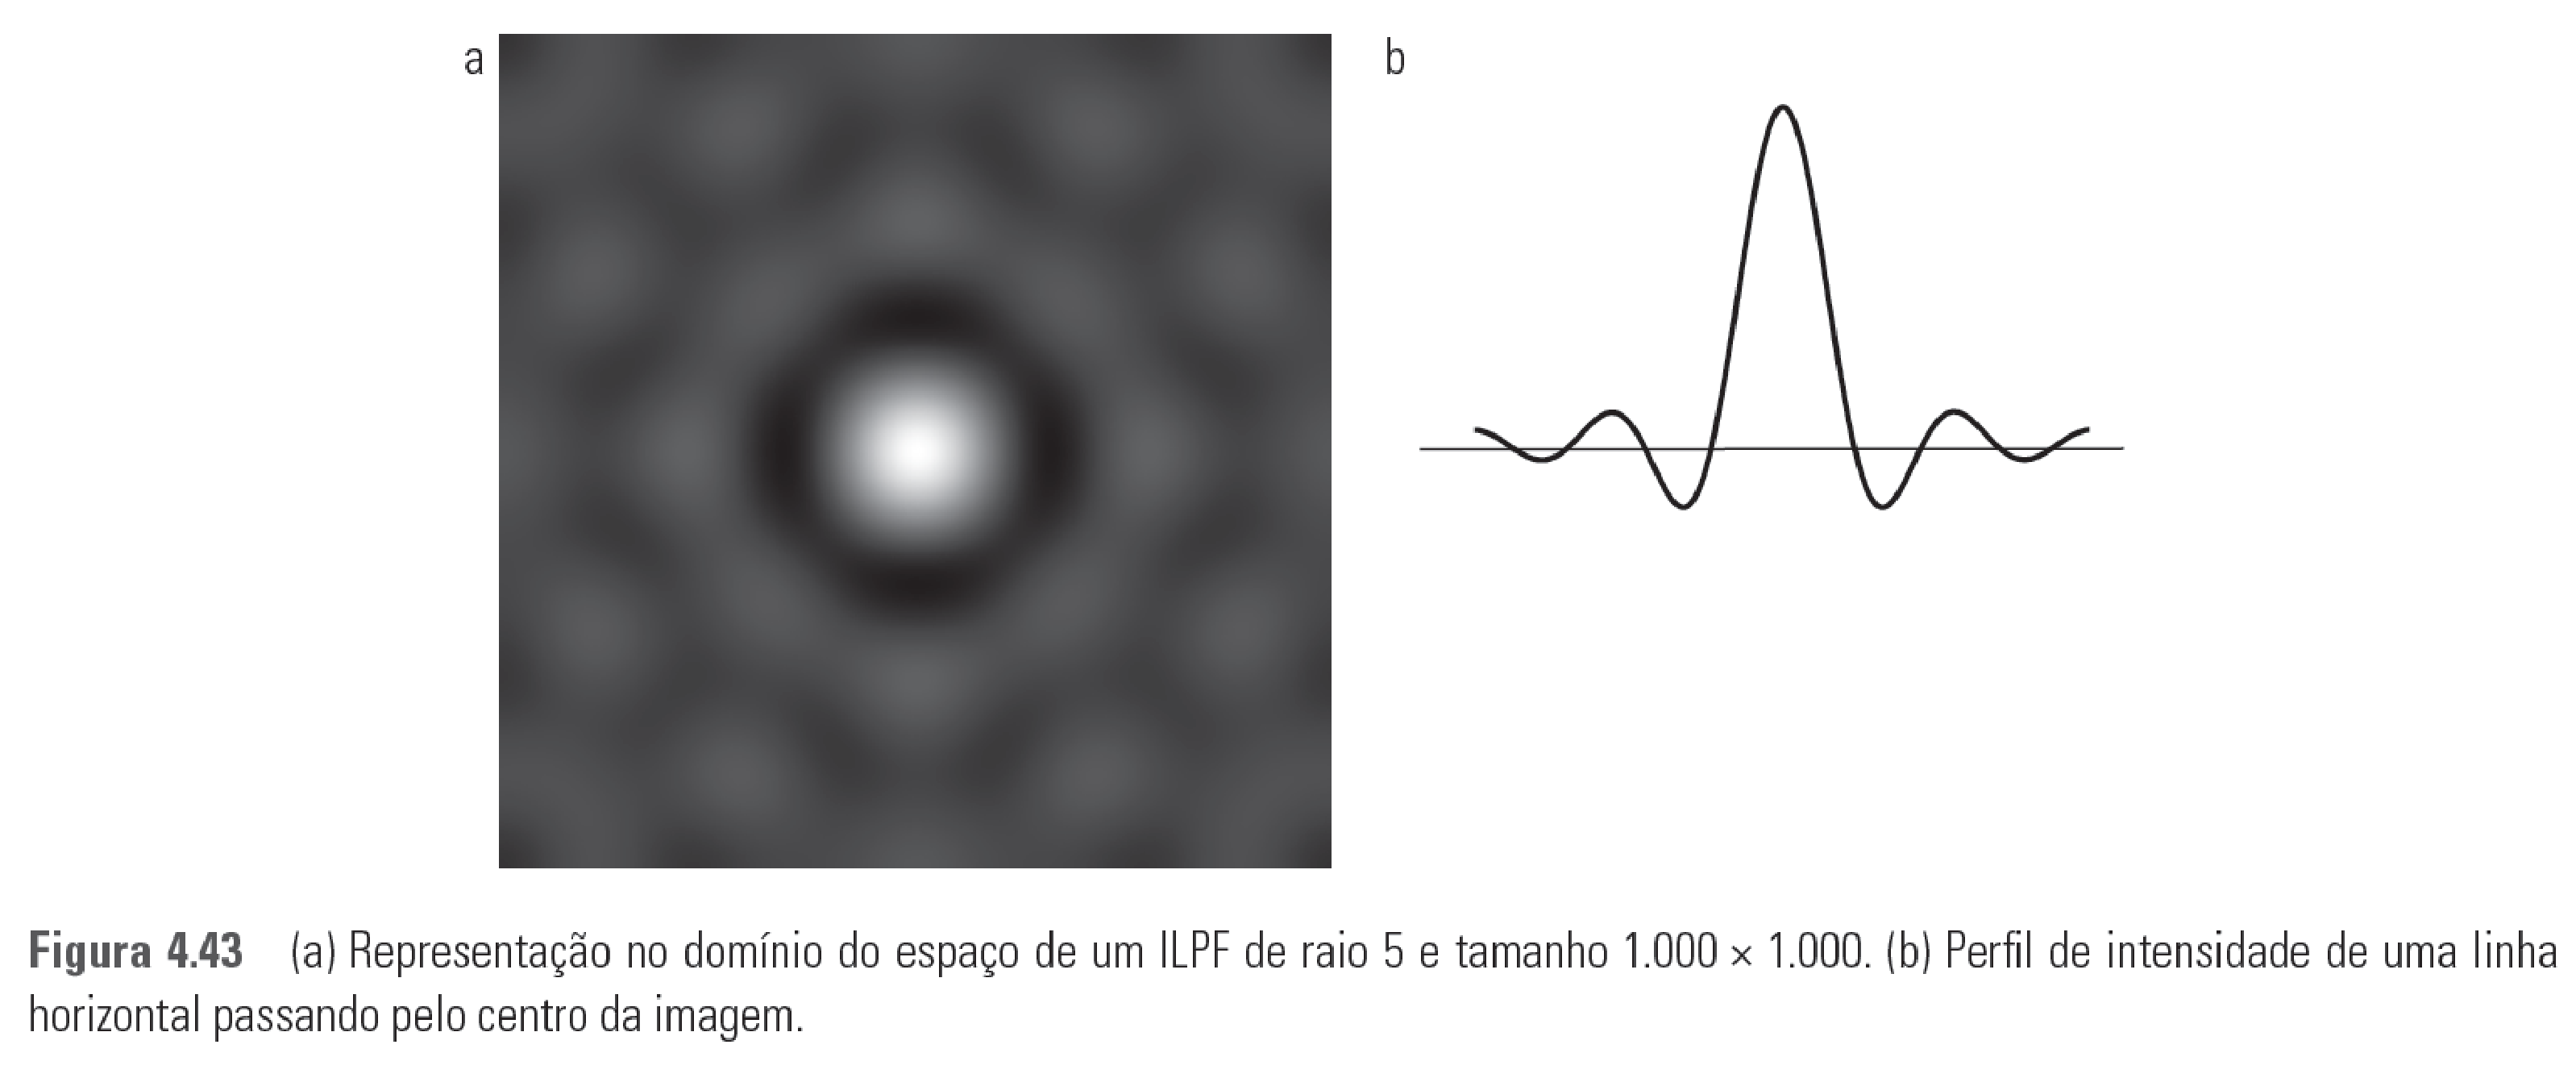
\includegraphics[width=0.95\textwidth]{figs/fig0443}
         \end{itemize}
      \end{slide}
      
      \begin{slide}[toc=]{Filtro passa baixa Butterworth}
         \begin{itemize}[type=1]
            \item Resposta em frequência
            \begin{equation*}
               H(u,v) = \frac{1}{1+\left[ D(u,v)/D_0\right]^{2n}}
            \end{equation*}
            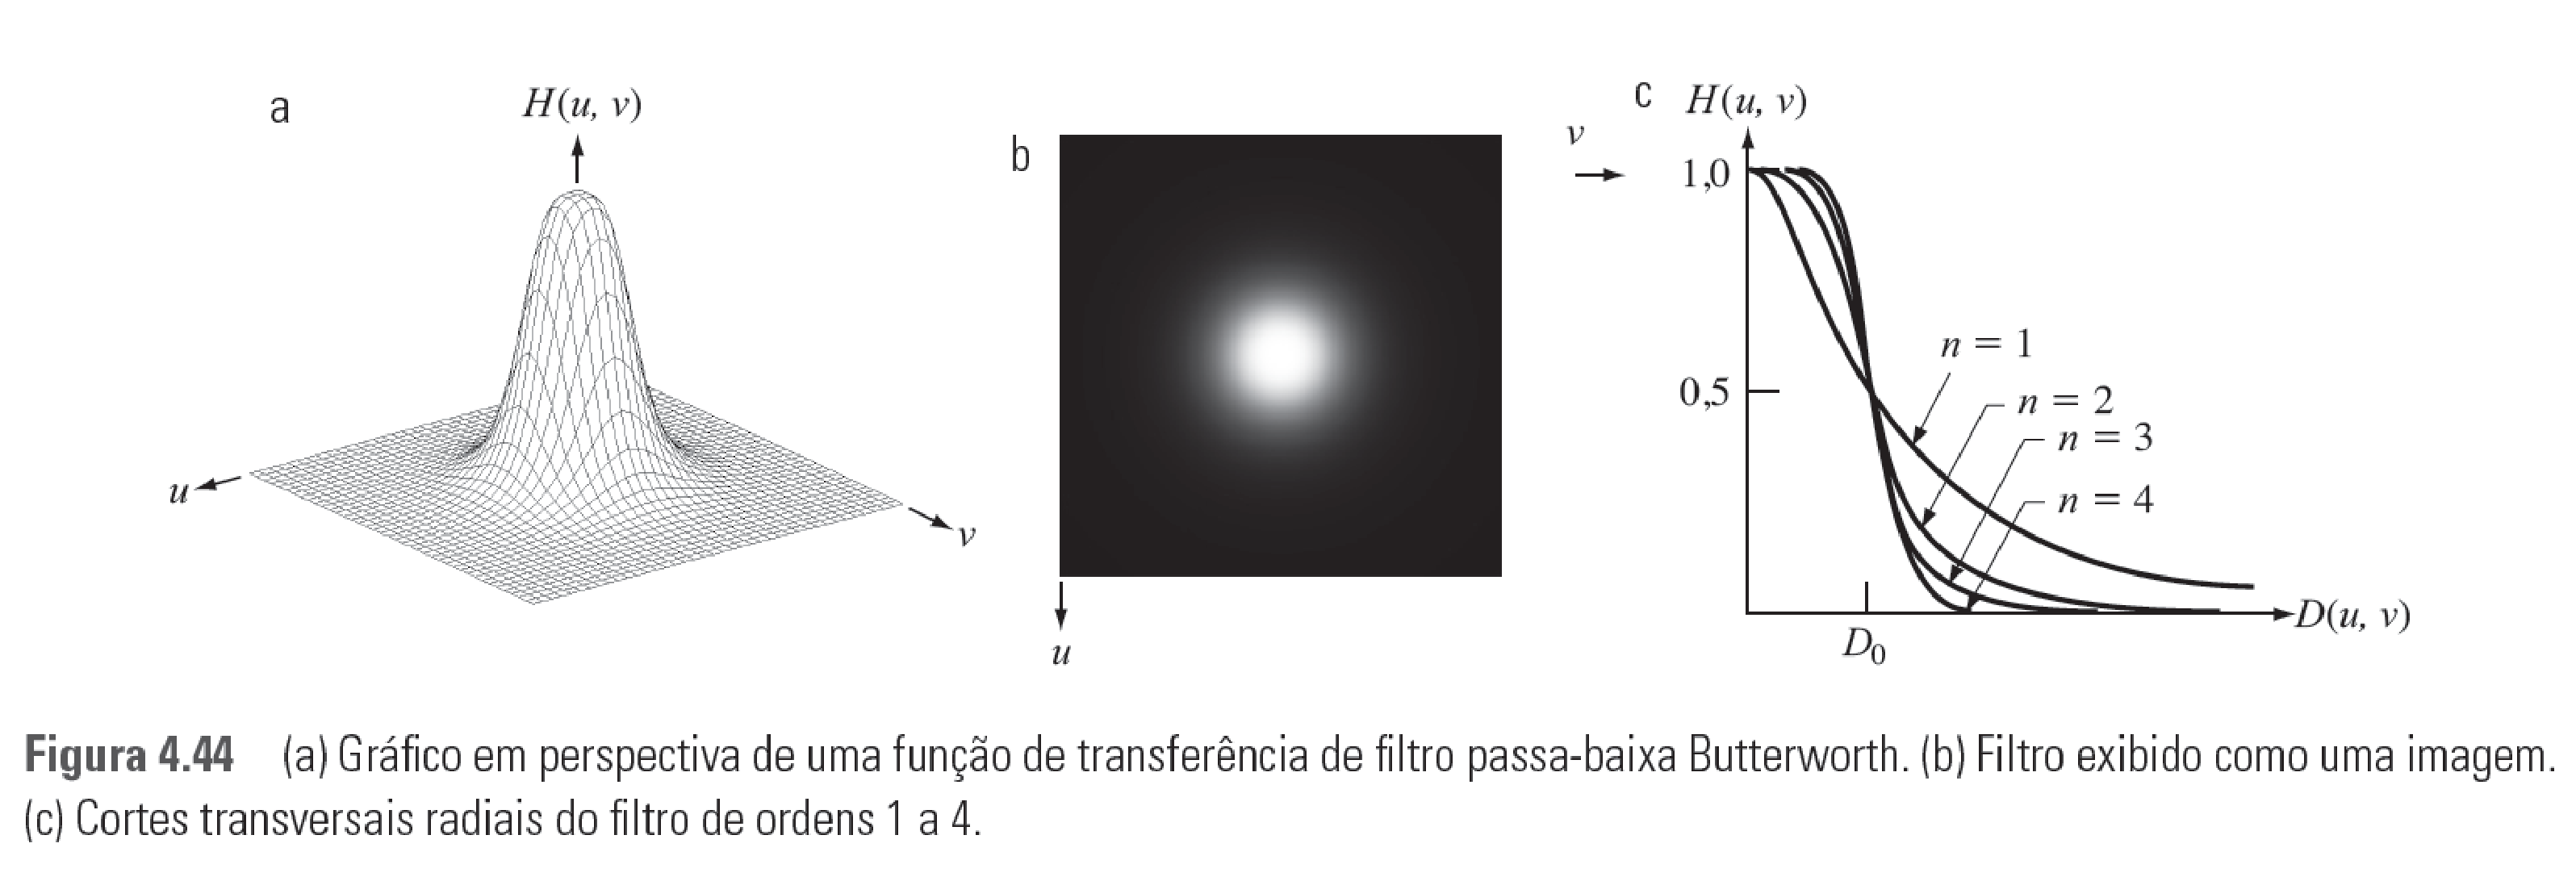
\includegraphics[width=0.95\textwidth]{figs/fig0444}
         \end{itemize}
      \end{slide}
      
      \begin{slide}[toc=]{Filtro passa baixa Butterworth}
         \begin{itemize}[type=1]
            \item Exemplos
         \end{itemize}
	      \begin{center}
            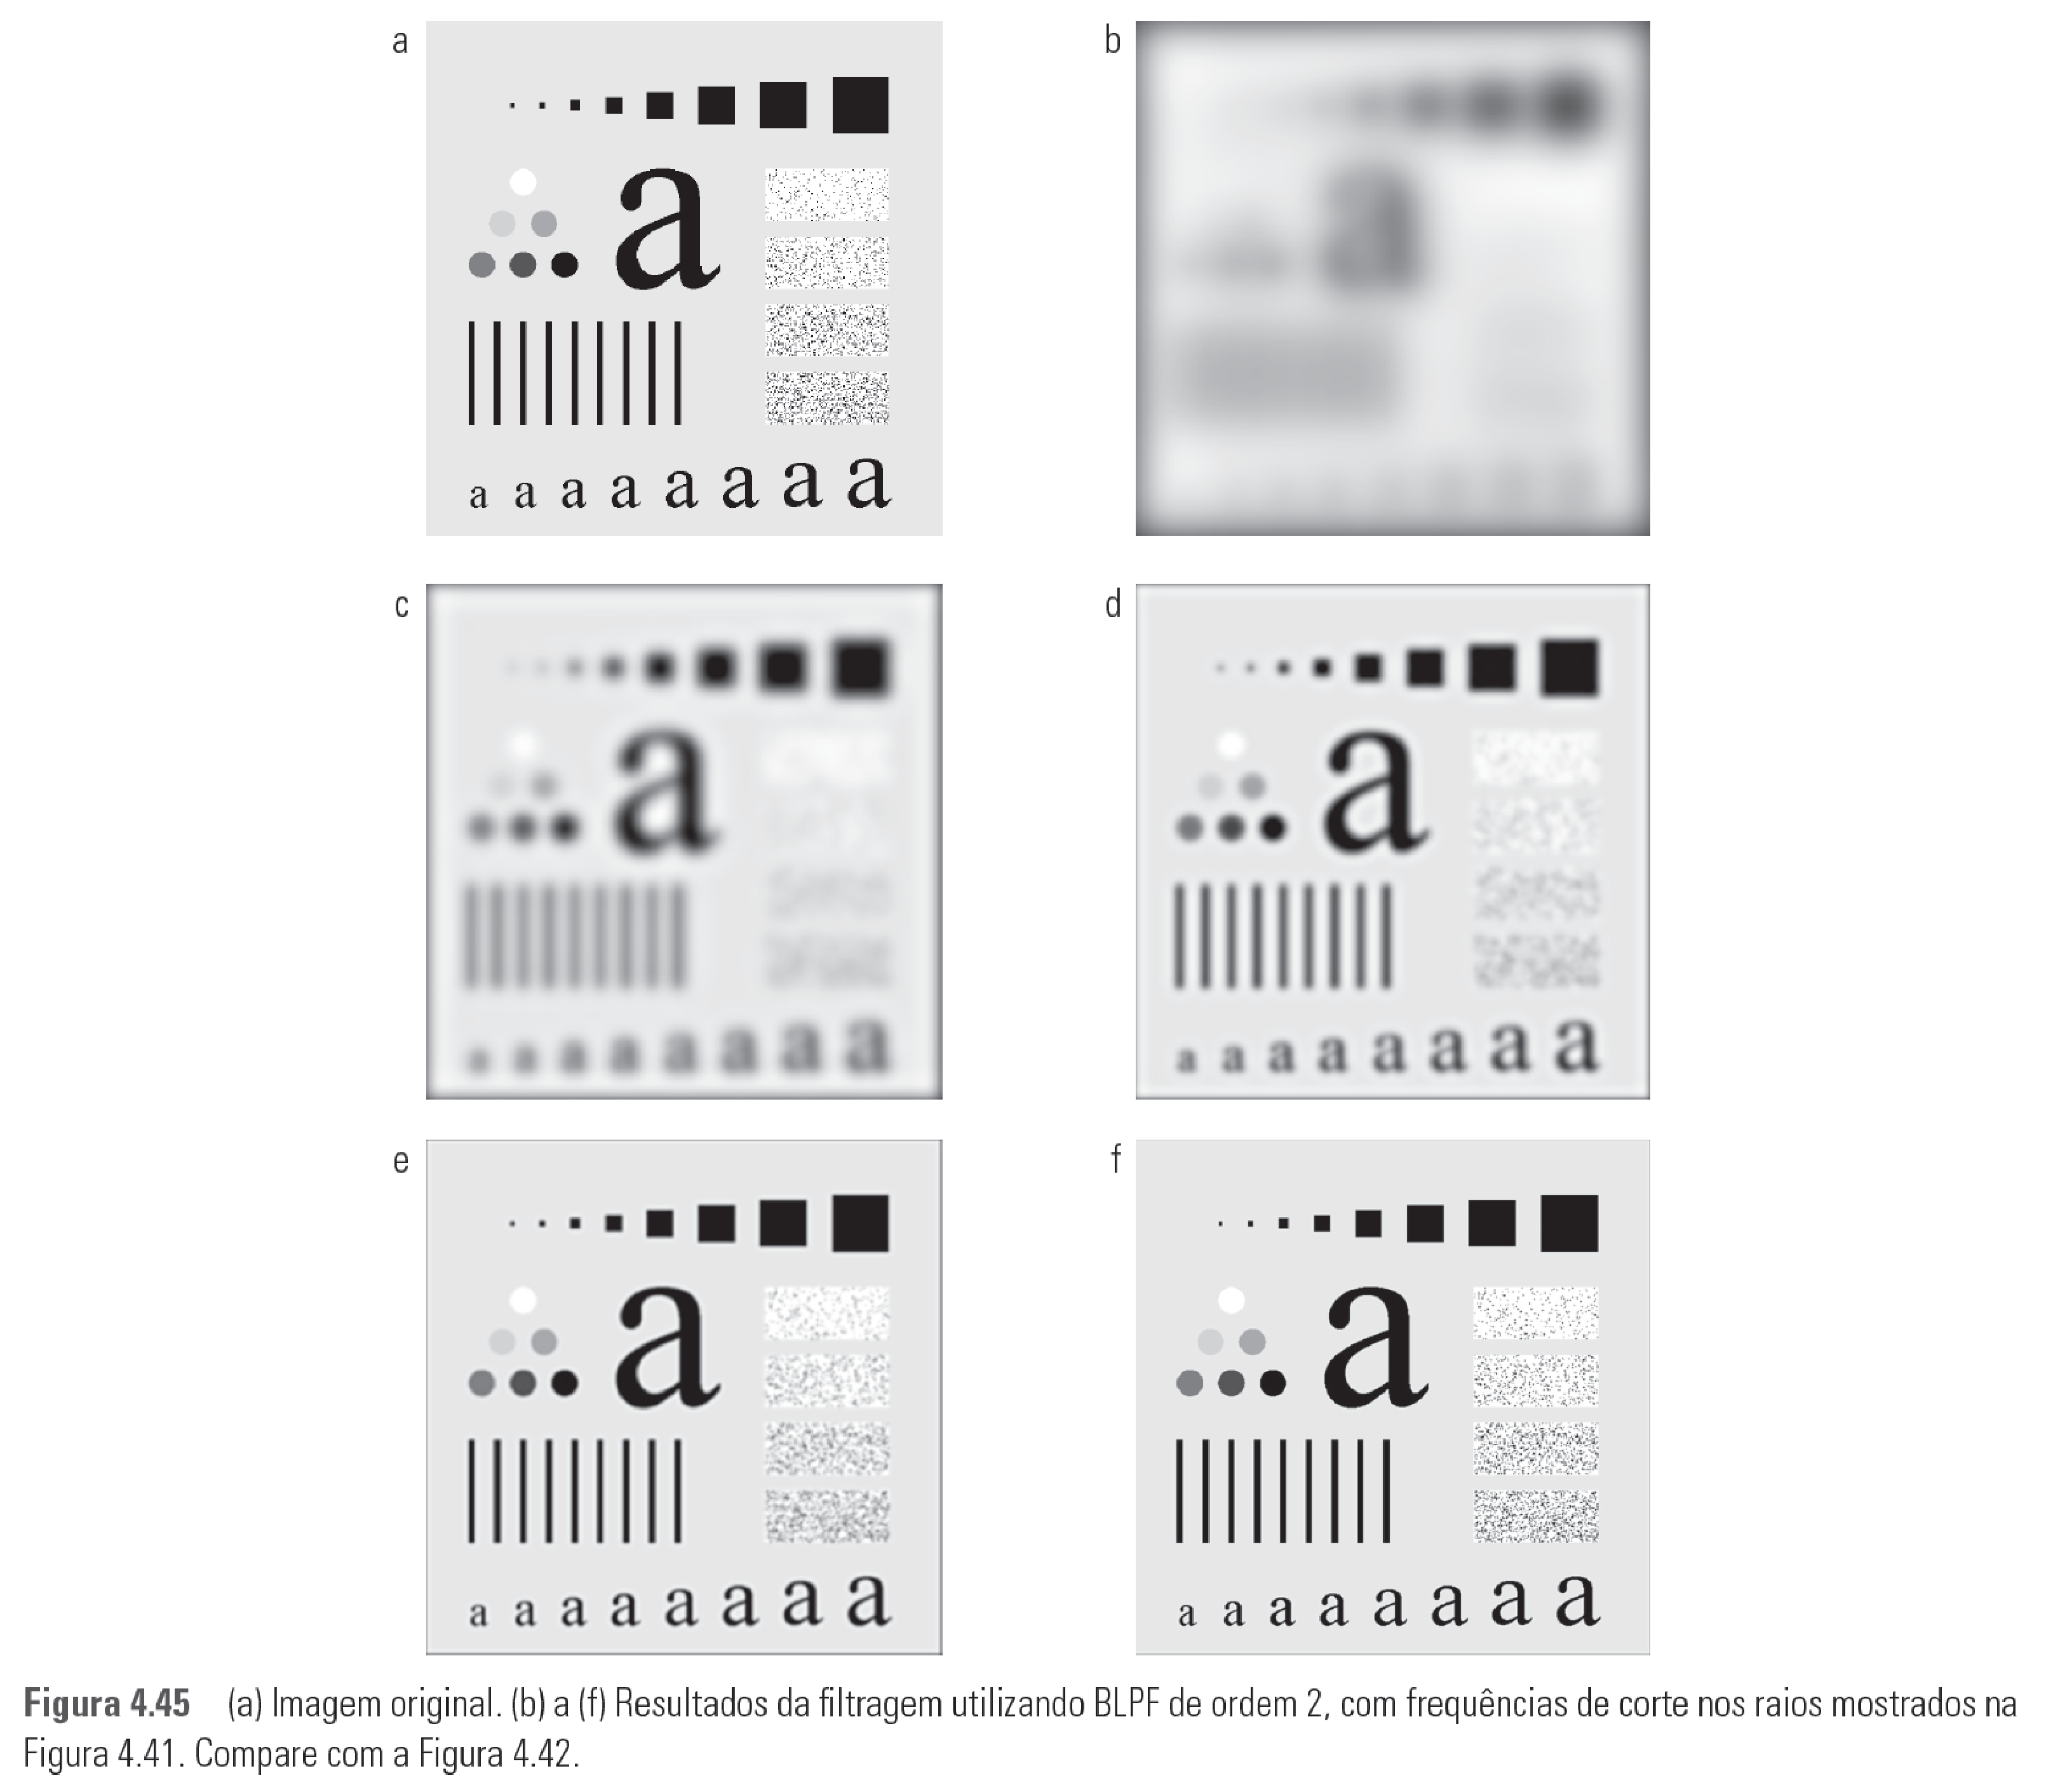
\includegraphics[width=0.55\textwidth]{figs/fig0445}
	      \end{center}
      \end{slide}
      
      \begin{slide}[toc=]{Filtro passa Butterworth}
         \begin{itemize}[type=1]
            \item Efeitos de anelamento (ringing)
            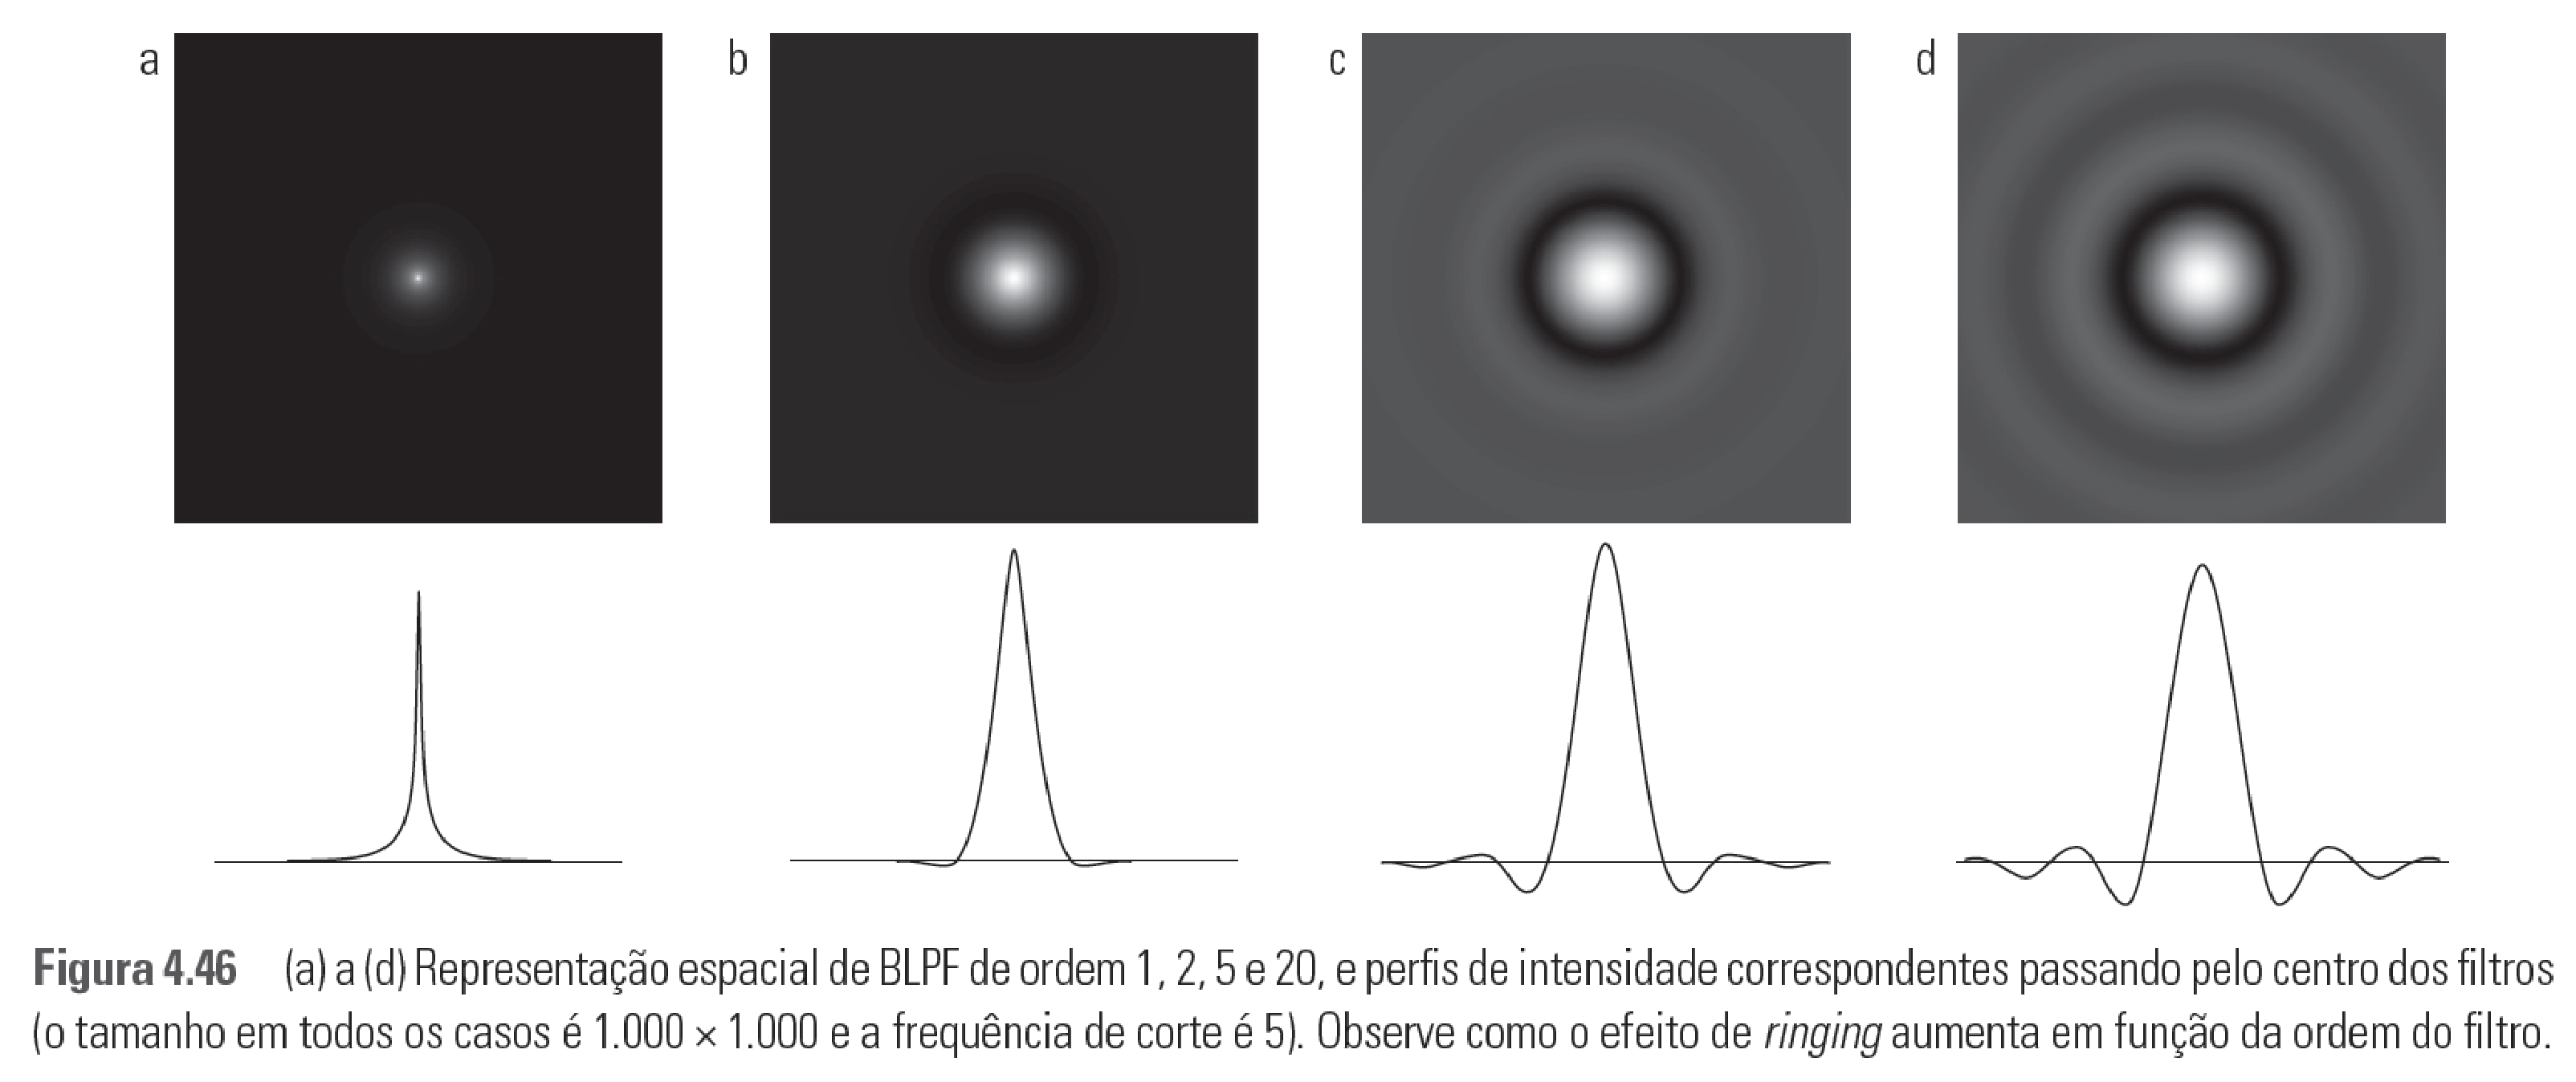
\includegraphics[width=0.95\textwidth]{figs/fig0446}
         \end{itemize}
      \end{slide}
      
      \begin{slide}[toc=]{Filtro passa baixa gaussiano}
         \begin{itemize}[type=1]
            \item Resposta em frequência
            \begin{equation*}
               H(u,v) = e^{-\frac{D^2(u,v)}{2D^2_0}}
            \end{equation*}
            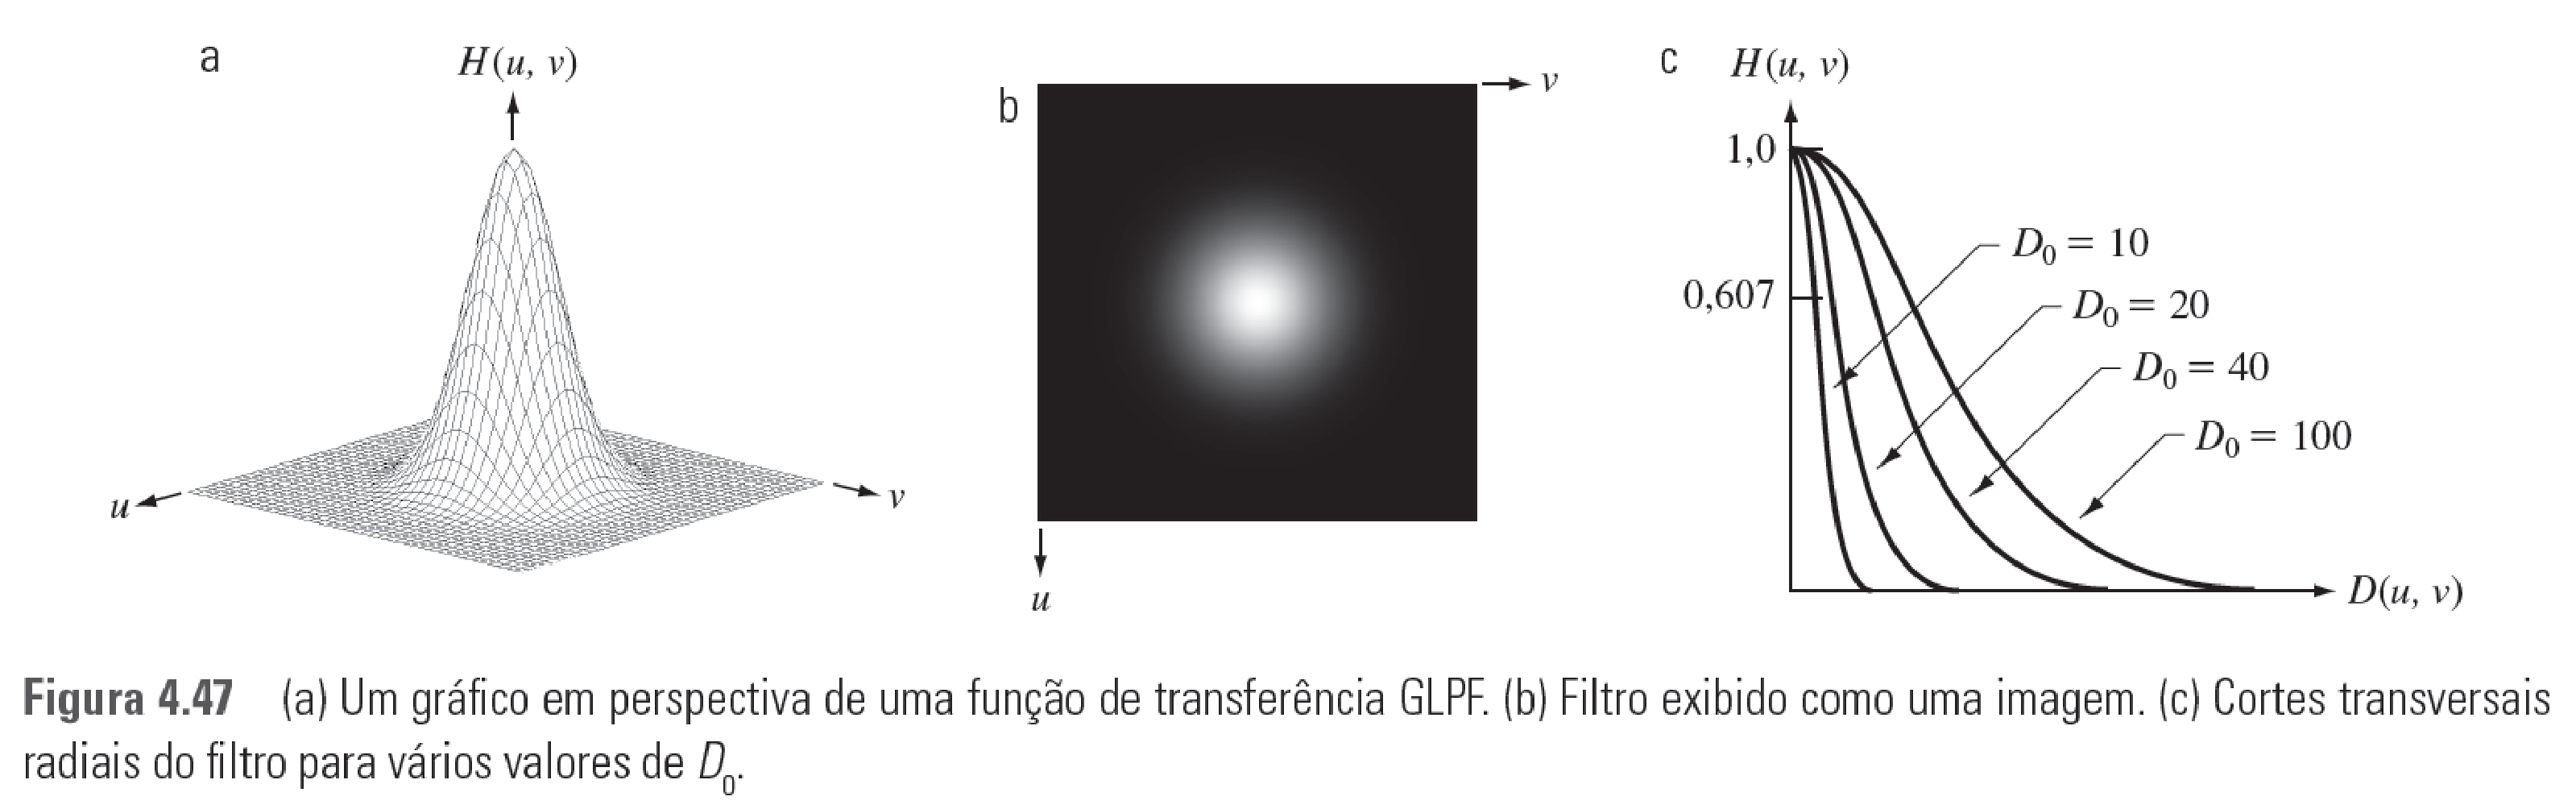
\includegraphics[width=0.95\textwidth]{figs/fig0447}
         \end{itemize}
      \end{slide}
      
      \begin{slide}[toc=]{Filtro passa baixa gaussiano}
         \begin{itemize}[type=1]
            \item Exemplos
         \end{itemize}
	      \begin{center}
            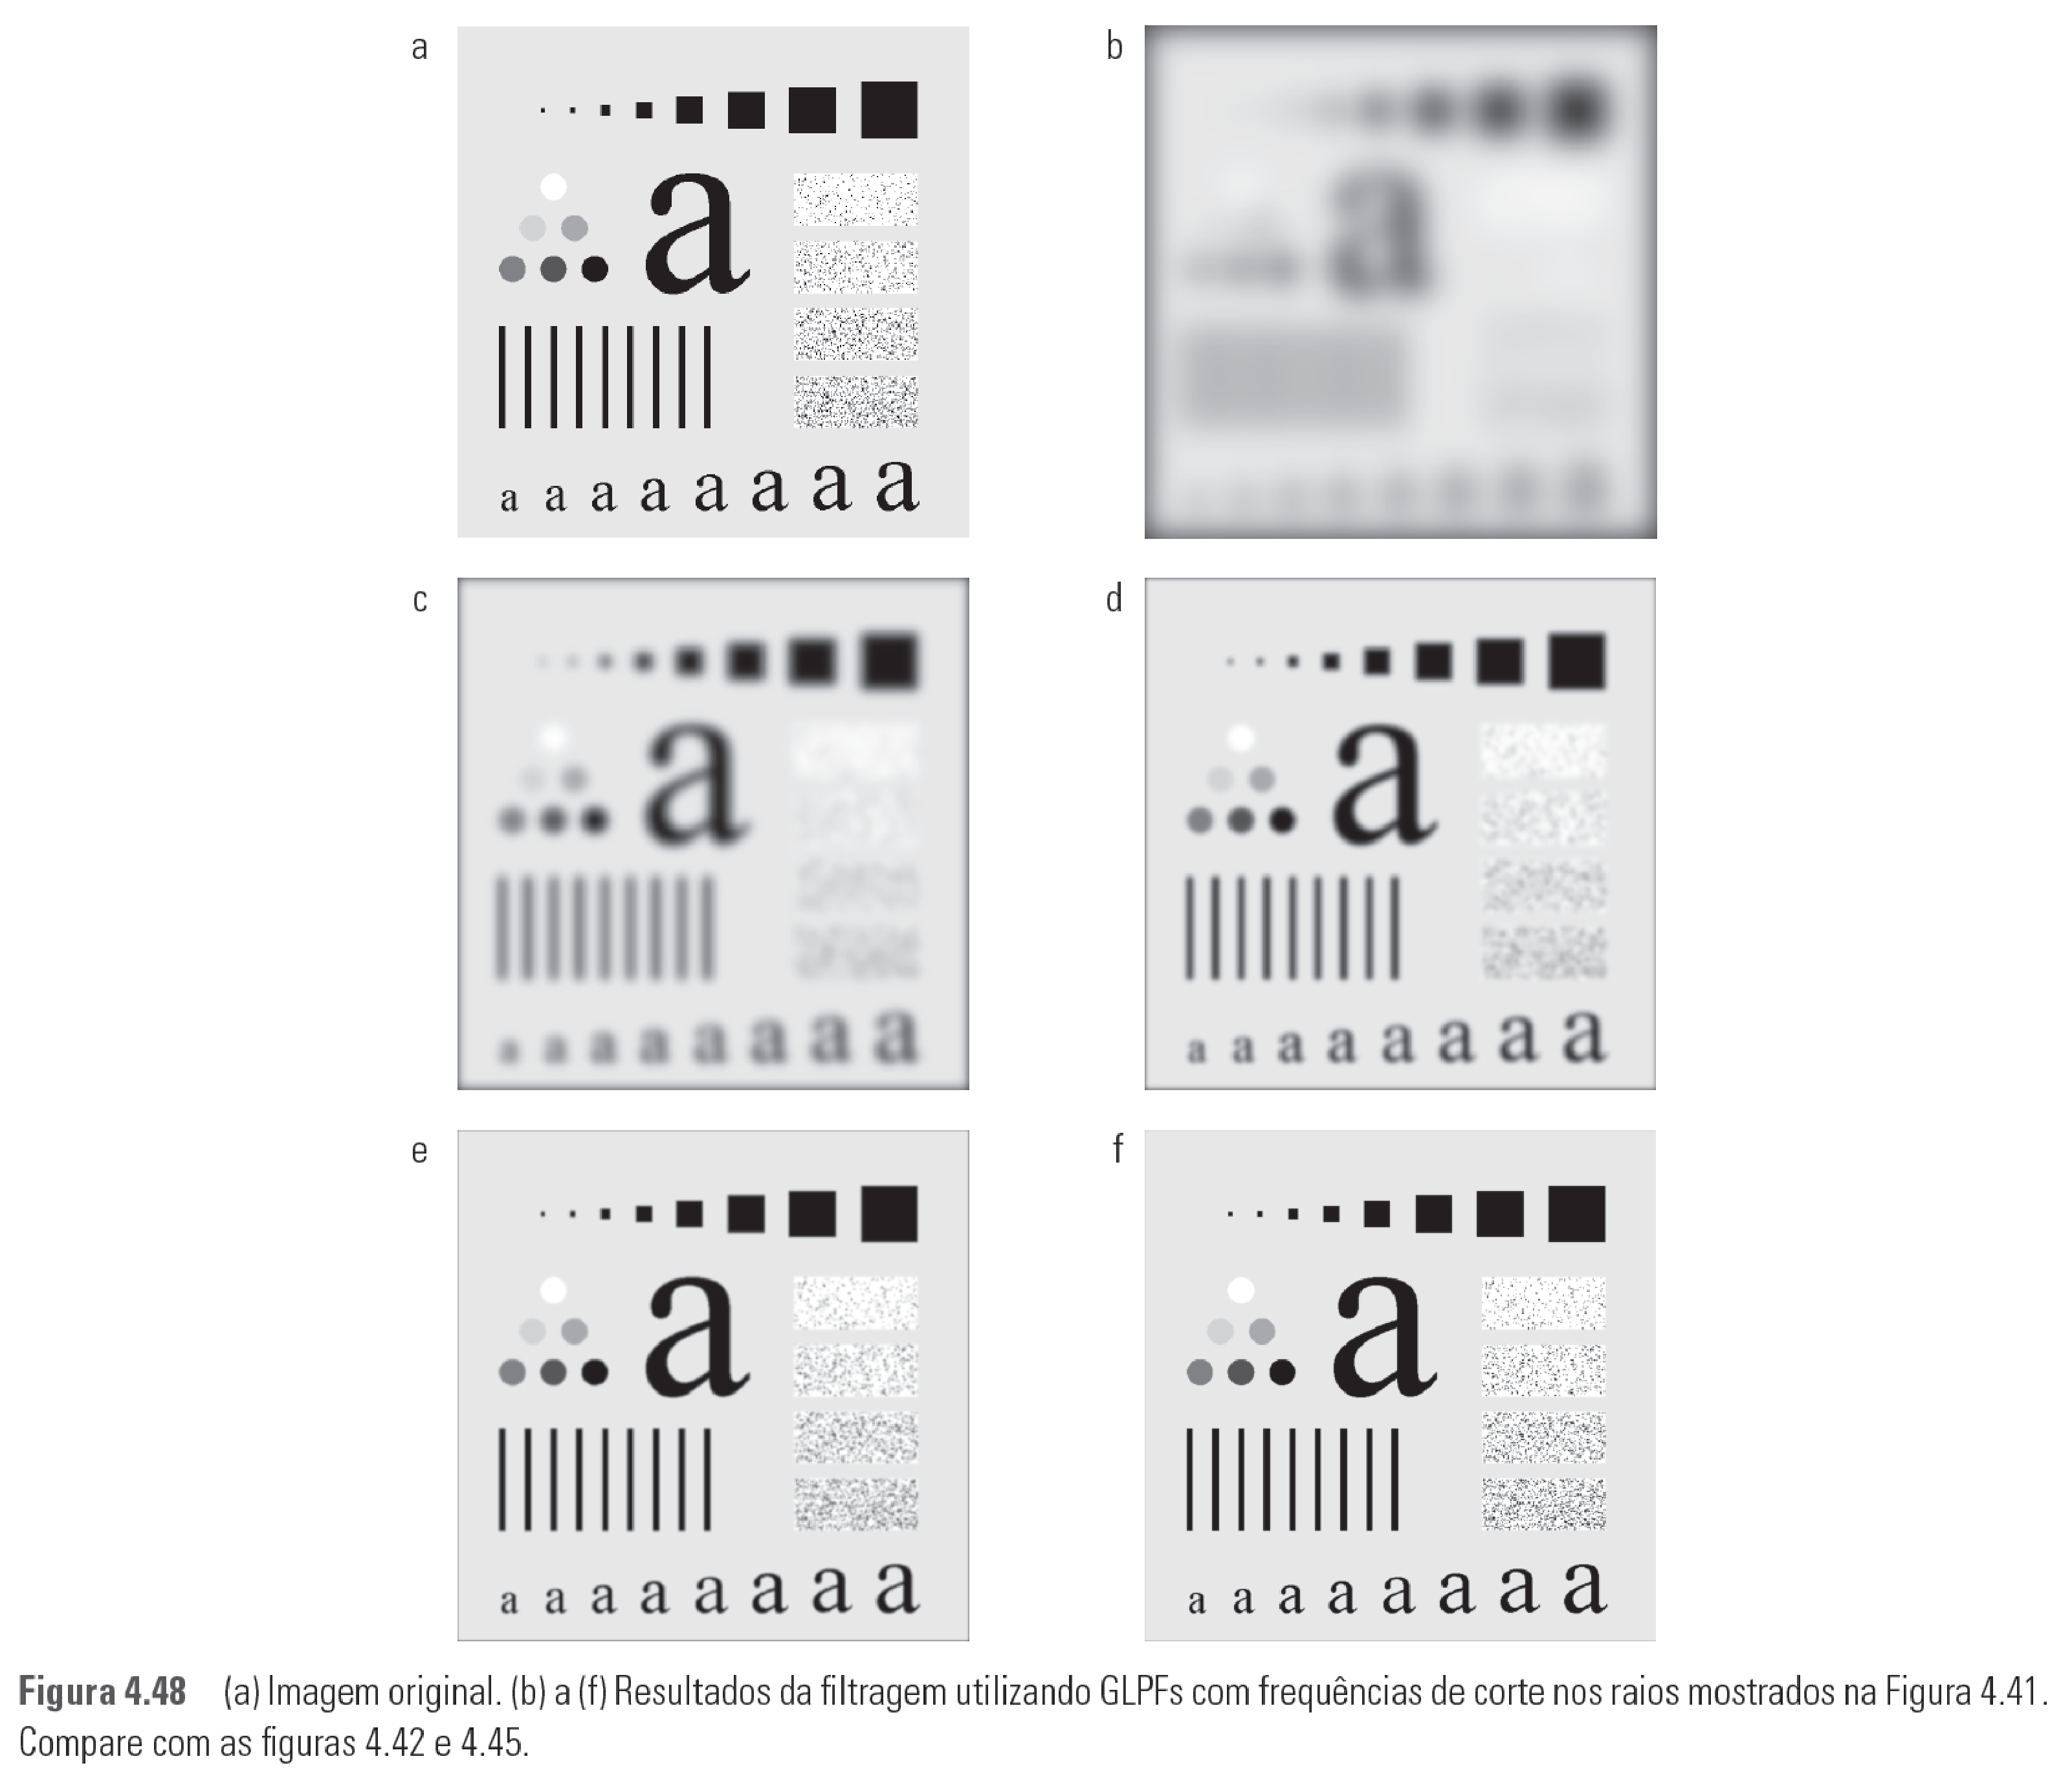
\includegraphics[width=0.55\textwidth]{figs/fig0448}
	      \end{center}
      \end{slide}
   
   \section[slide=true]{Aguçamento de imagens}
      \begin{slide}[toc=]{Filtros passa alta}
         \begin{itemize}[type=1]
            \item Passa alta ideal
            \begin{equation*}
               H(u,v) = \begin{cases}
                           1& \text{se }D(u,v)> D_0\\
                           0& \text{se }D(u,v)\leq D_0
                        \end{cases}
            \end{equation*}
            \item Passa alta Butterworth
            \begin{equation*}
               H(u,v) = \frac{1}{1+\left[ D_0/D(u,v)\right]^{2n}}
            \end{equation*}
            \item Passa alta gaussiano
            \begin{equation*}
               H(u,v) = 1-e^{-\frac{D^2(u,v)}{2D^2_0}}
            \end{equation*}
         \end{itemize}
      \end{slide}
      
      \begin{slide}[toc=]{Filtros passa alta}
         \begin{itemize}[type=1]
            \item Respostas em frequência
         \end{itemize}
	      \begin{center}
		      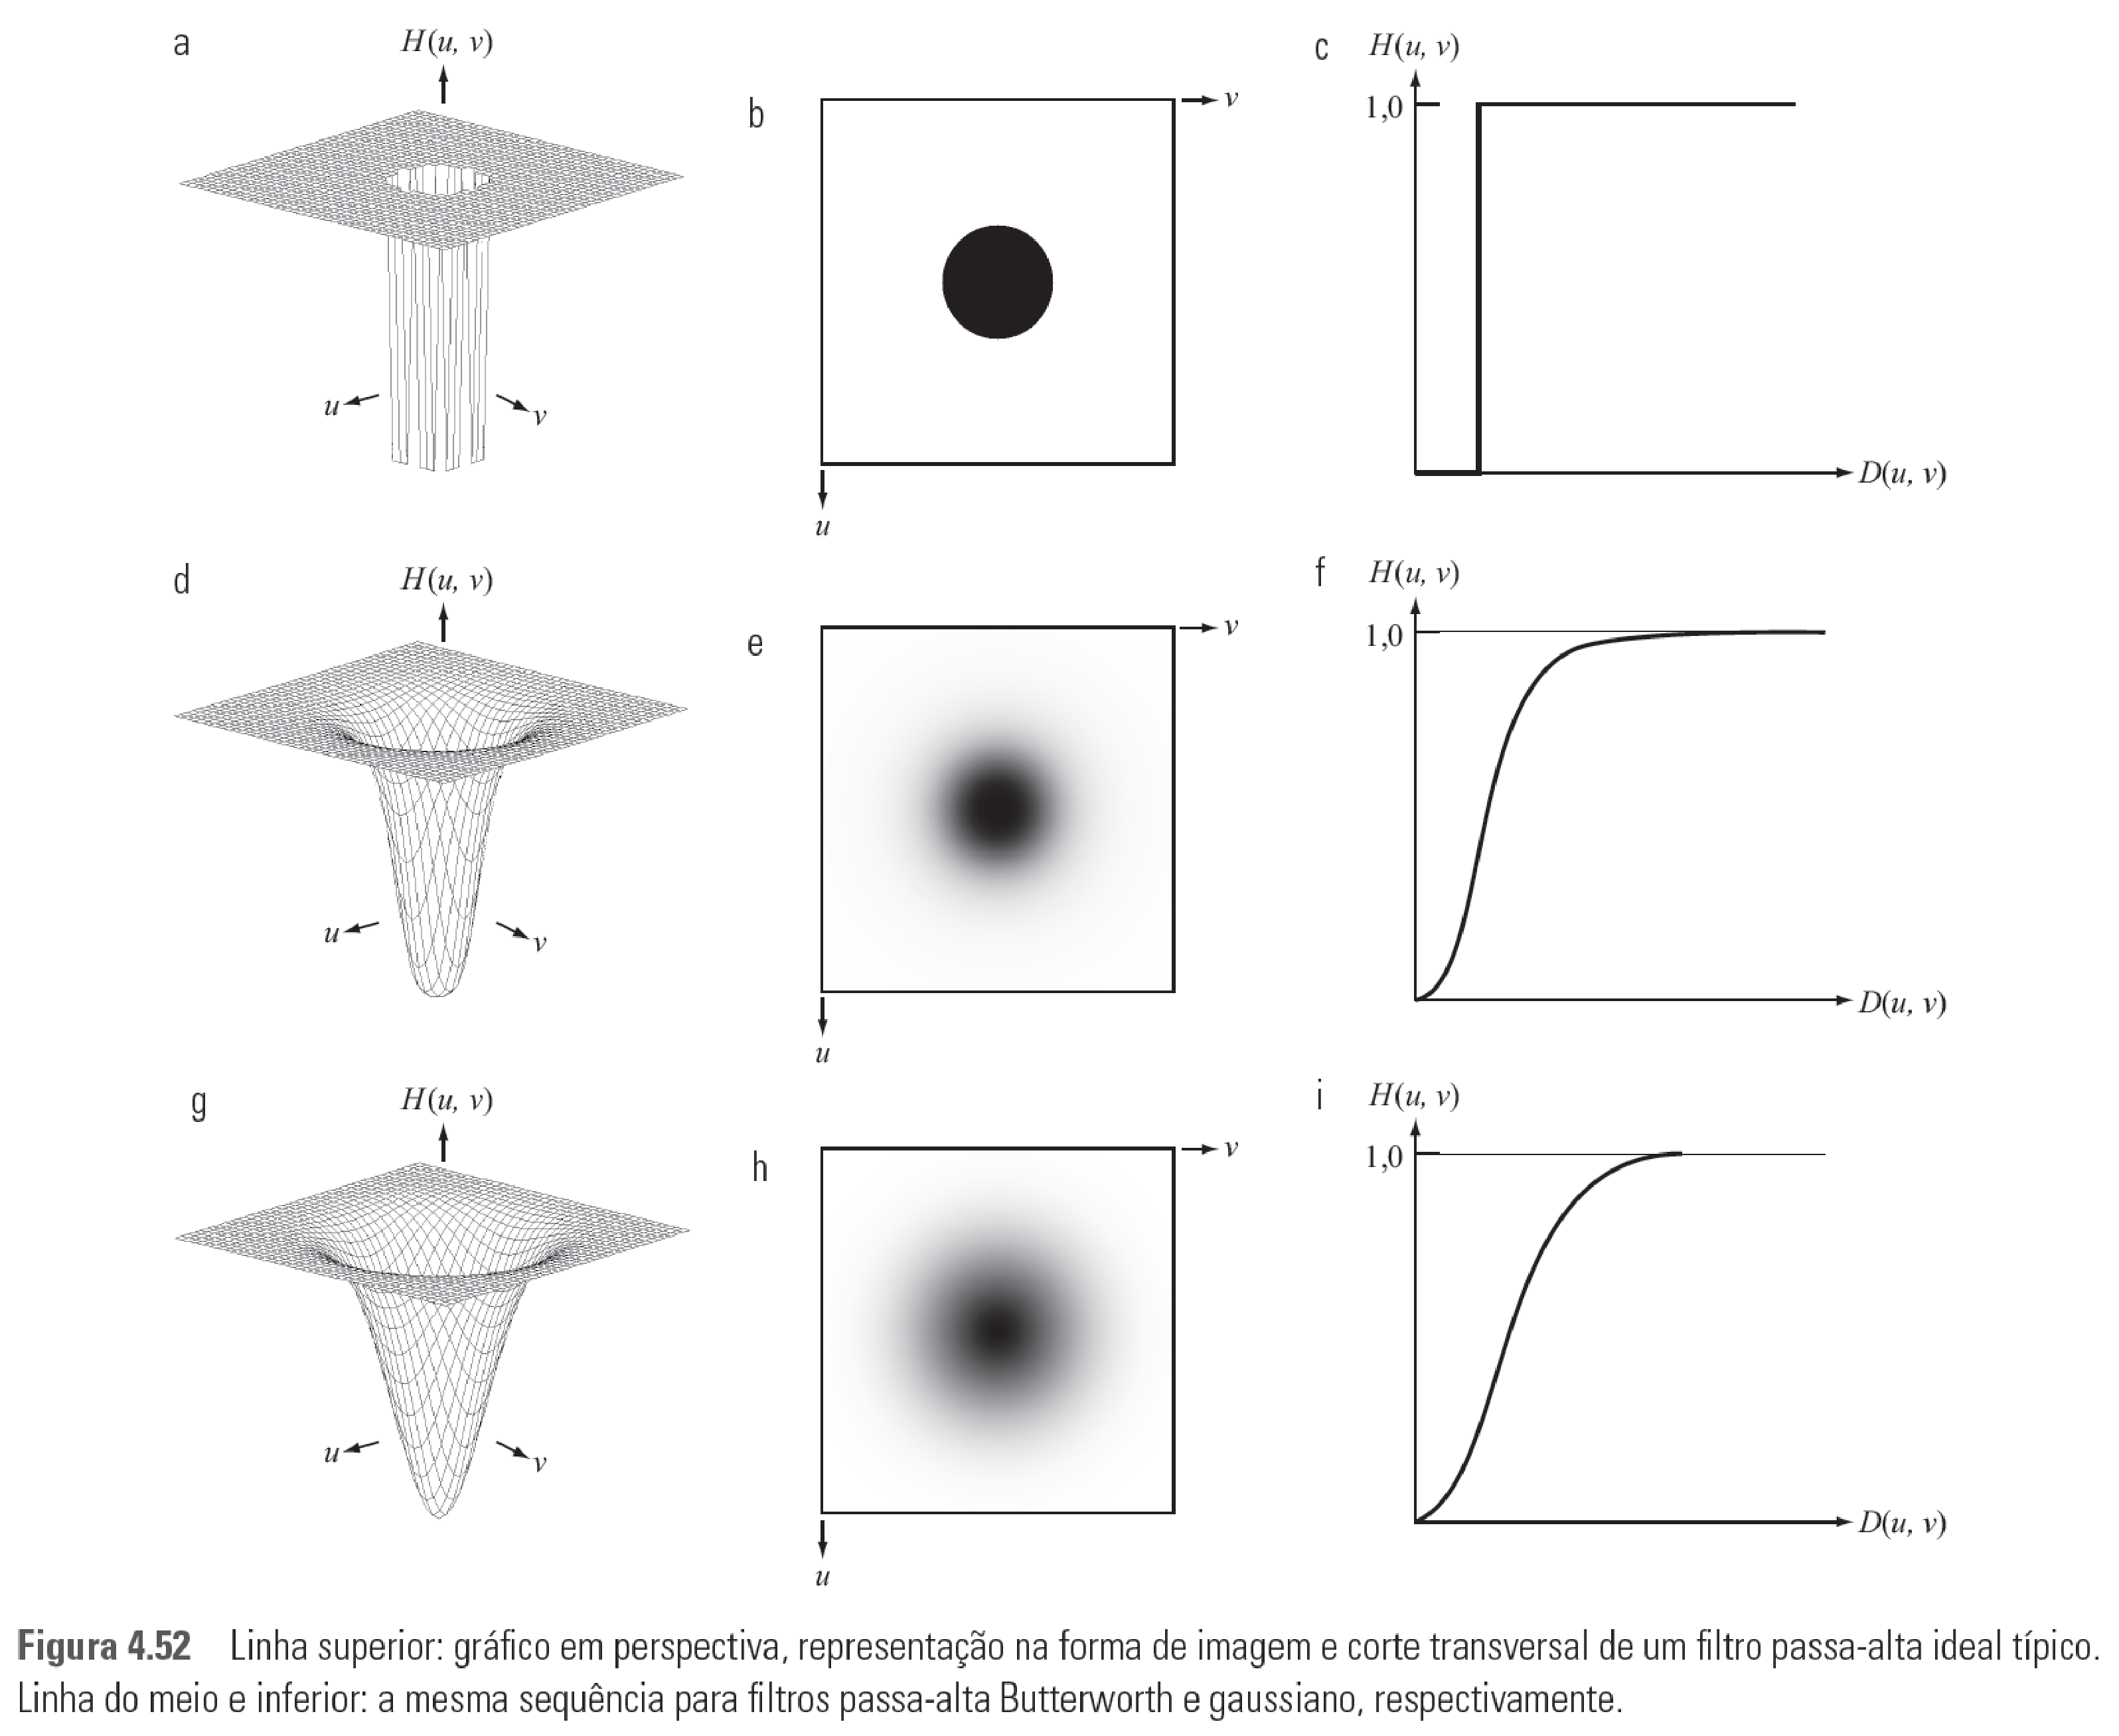
\includegraphics[height=0.7\textheight]{figs/fig0452}
	      \end{center}
      \end{slide}
      
      \begin{slide}[toc=]{Filtros passa alta}
         \begin{itemize}[type=1]
            \item Respostas ao impulso
            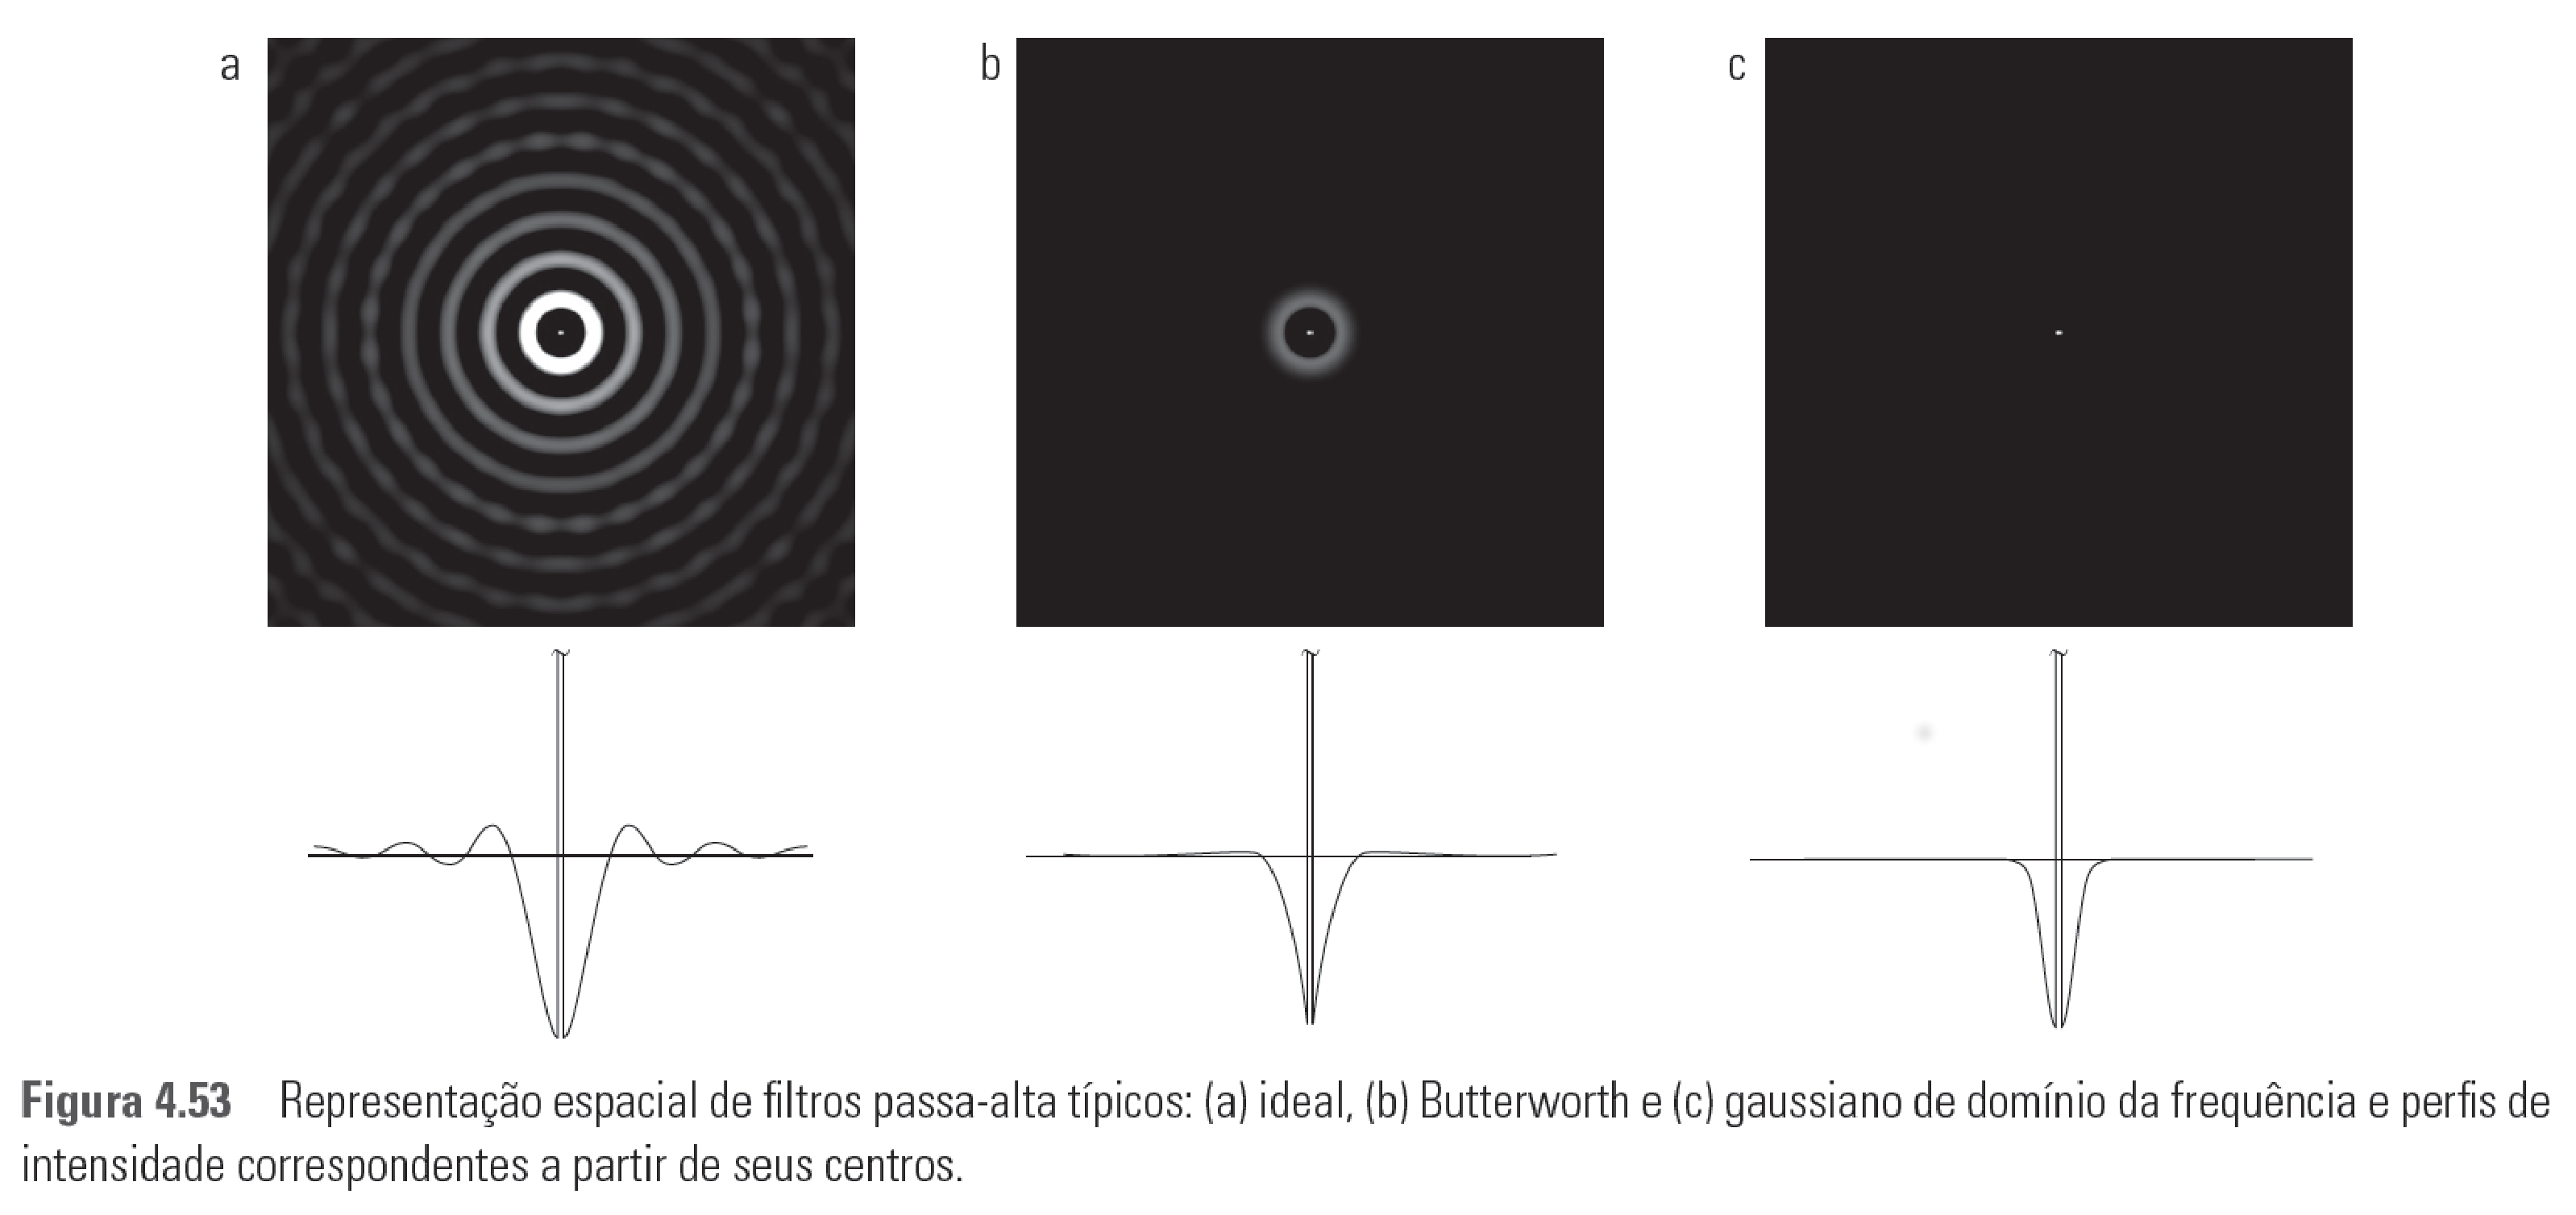
\includegraphics[width=0.95\textwidth]{figs/fig0453}
         \end{itemize}
      \end{slide}
      
      \begin{slide}[toc=]{Exemplos}
         \begin{itemize}[type=1]
            \item Passa alta ideal
	      \begin{center}
            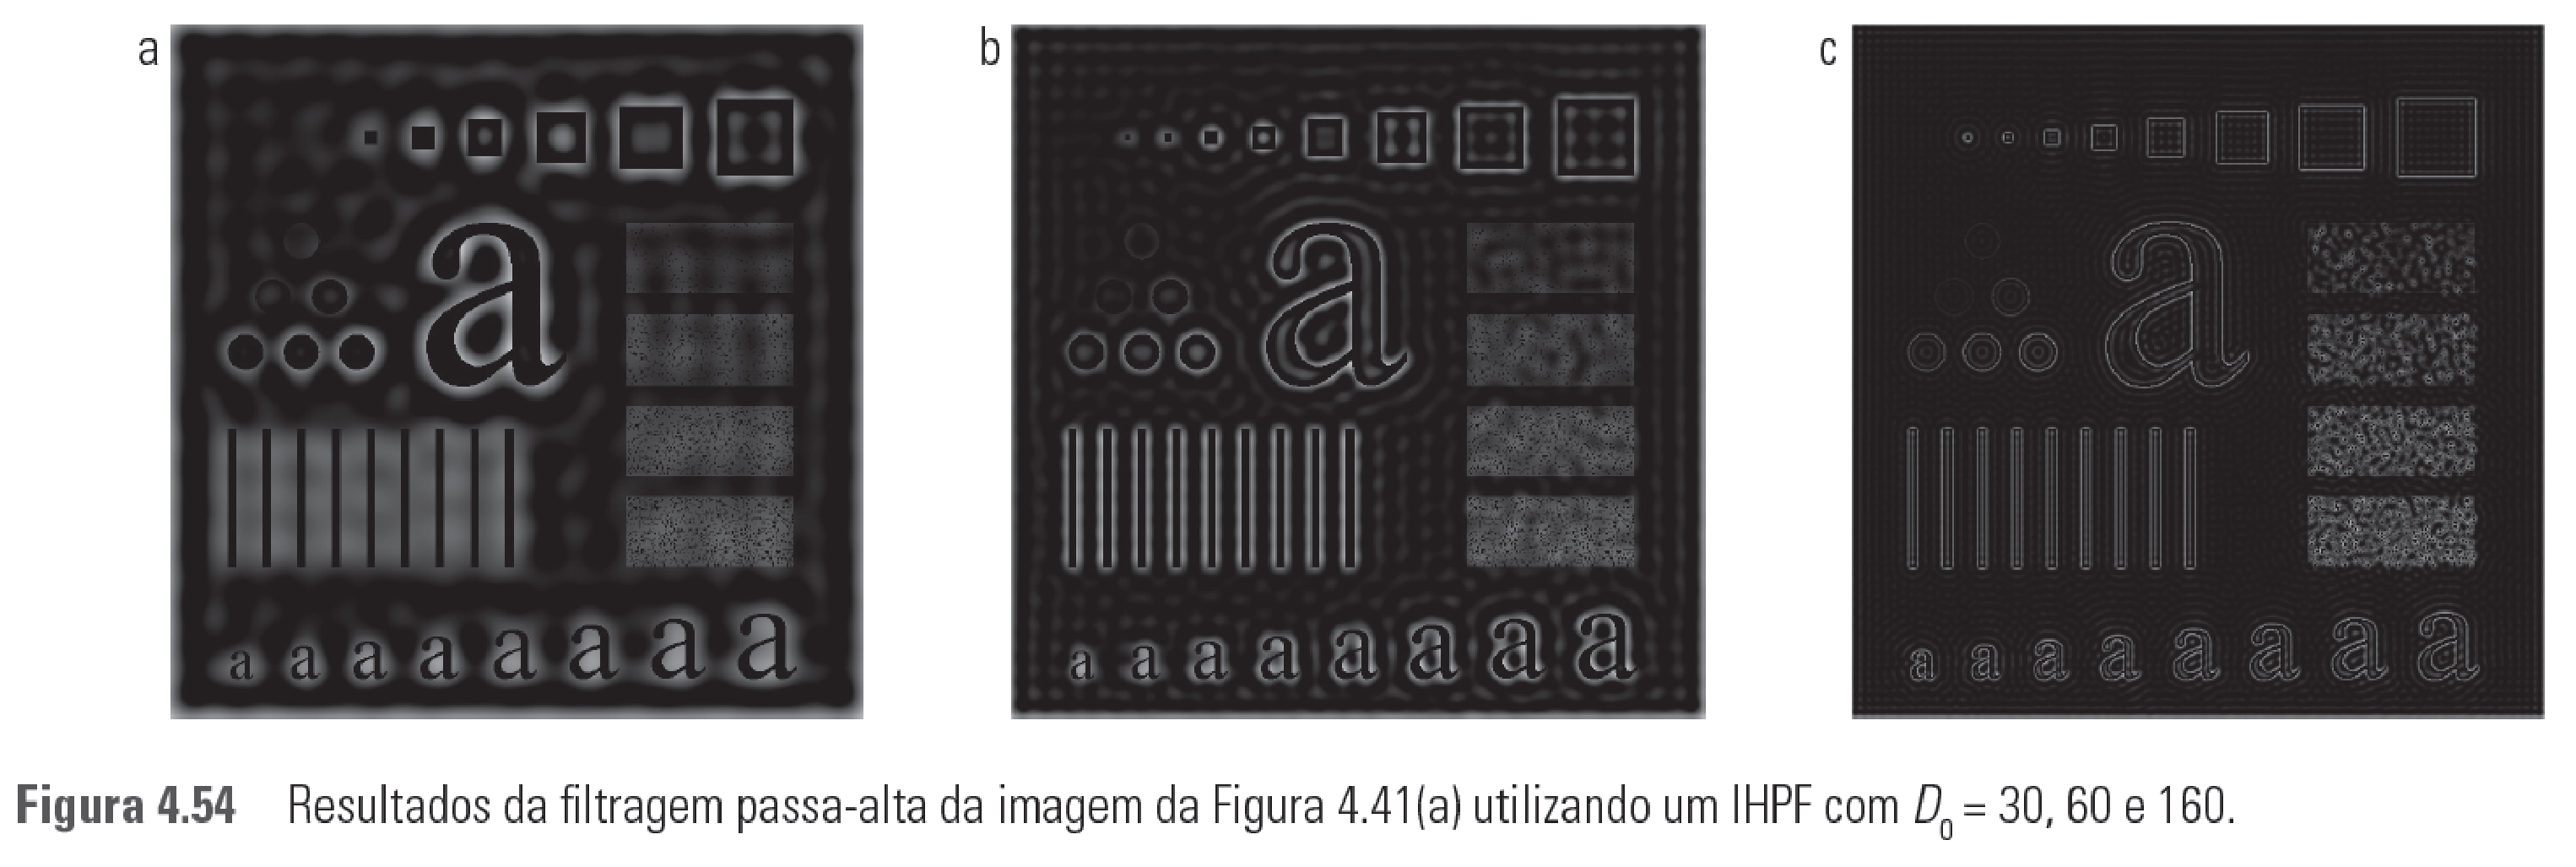
\includegraphics[width=0.65\textwidth]{figs/fig0454}
	      \end{center}
            \item Passa alta Butterworth
	      \begin{center}
            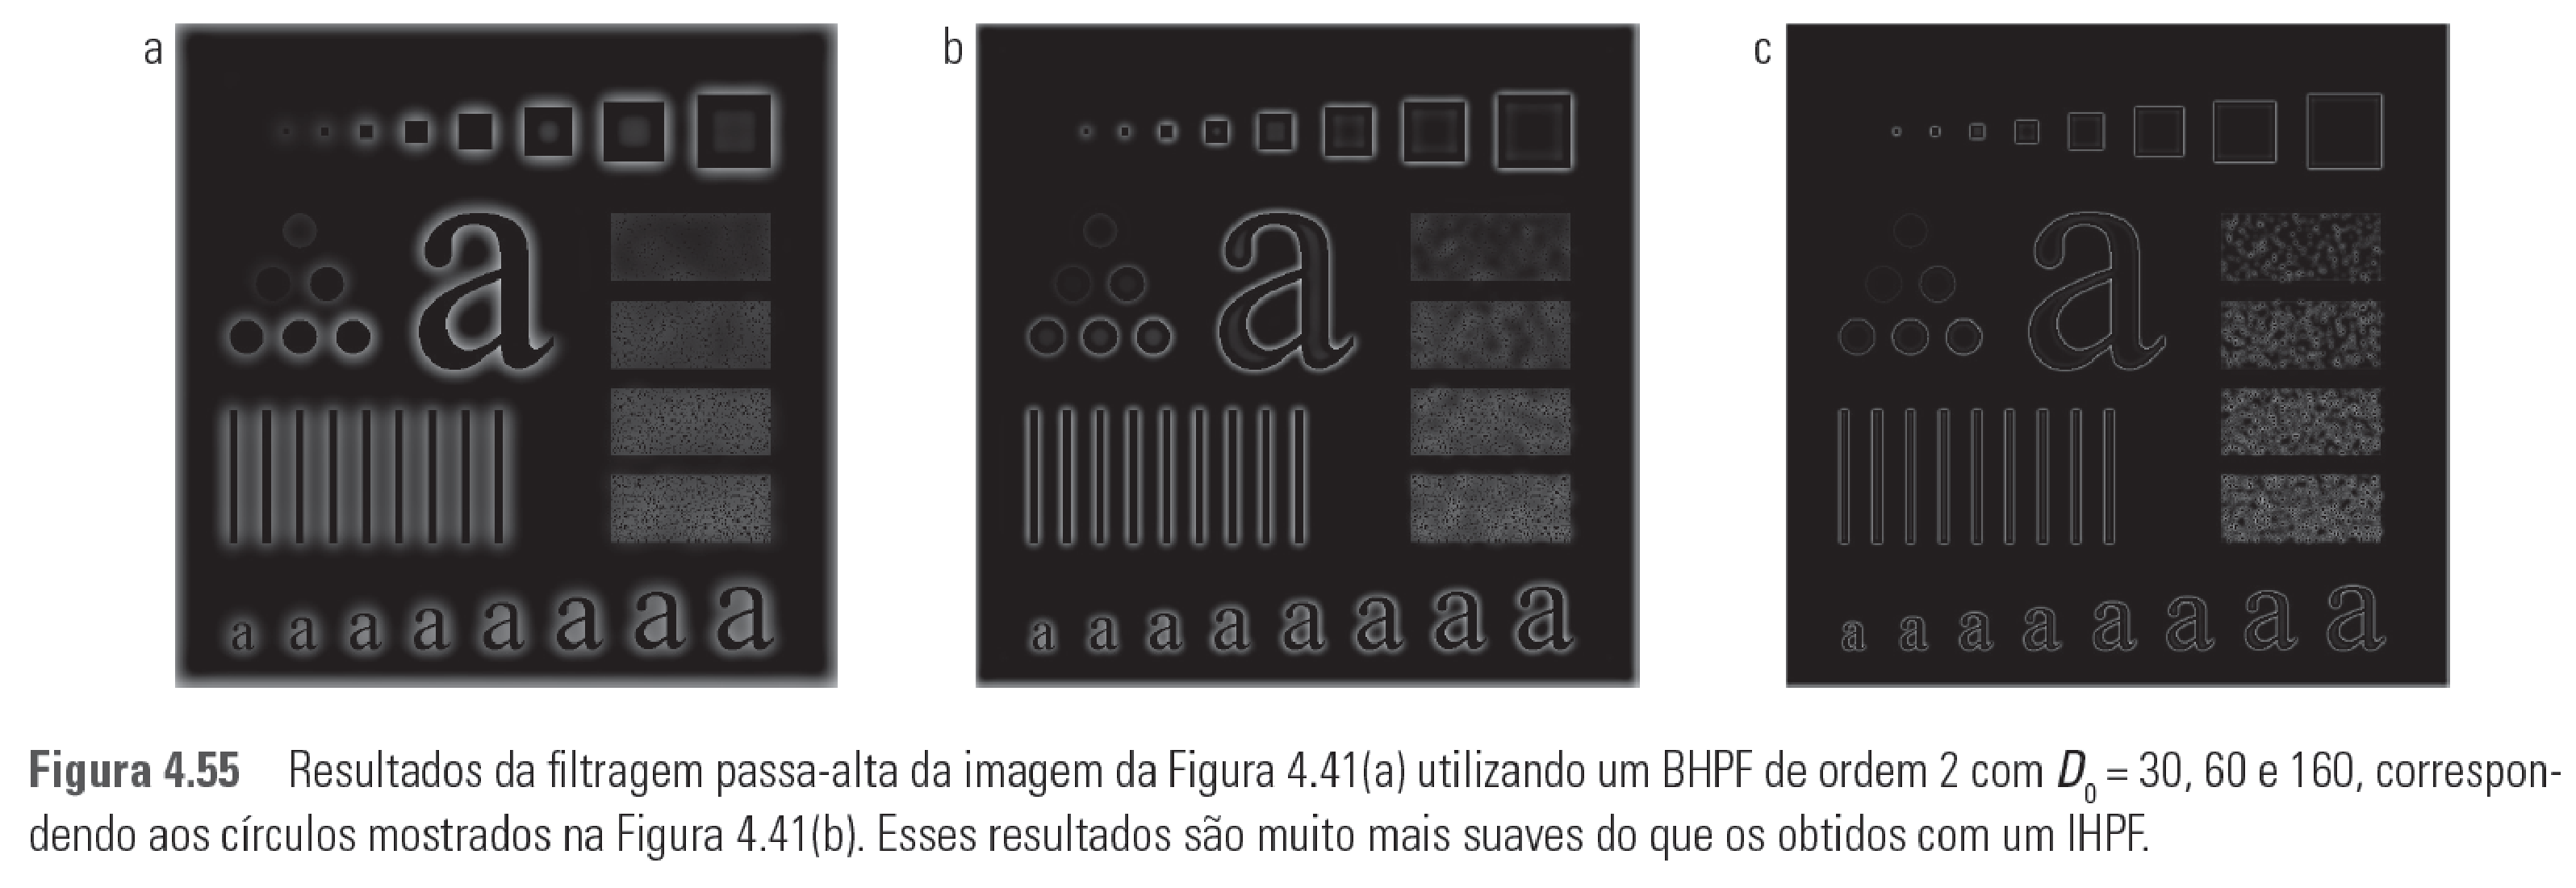
\includegraphics[width=0.65\textwidth]{figs/fig0455}
	      \end{center}
         \end{itemize}
      \end{slide}
      
      \begin{slide}[toc=]{Exemplos}
         \begin{itemize}[type=1]
            \item Passa alta gaussiano
	      \begin{center}
            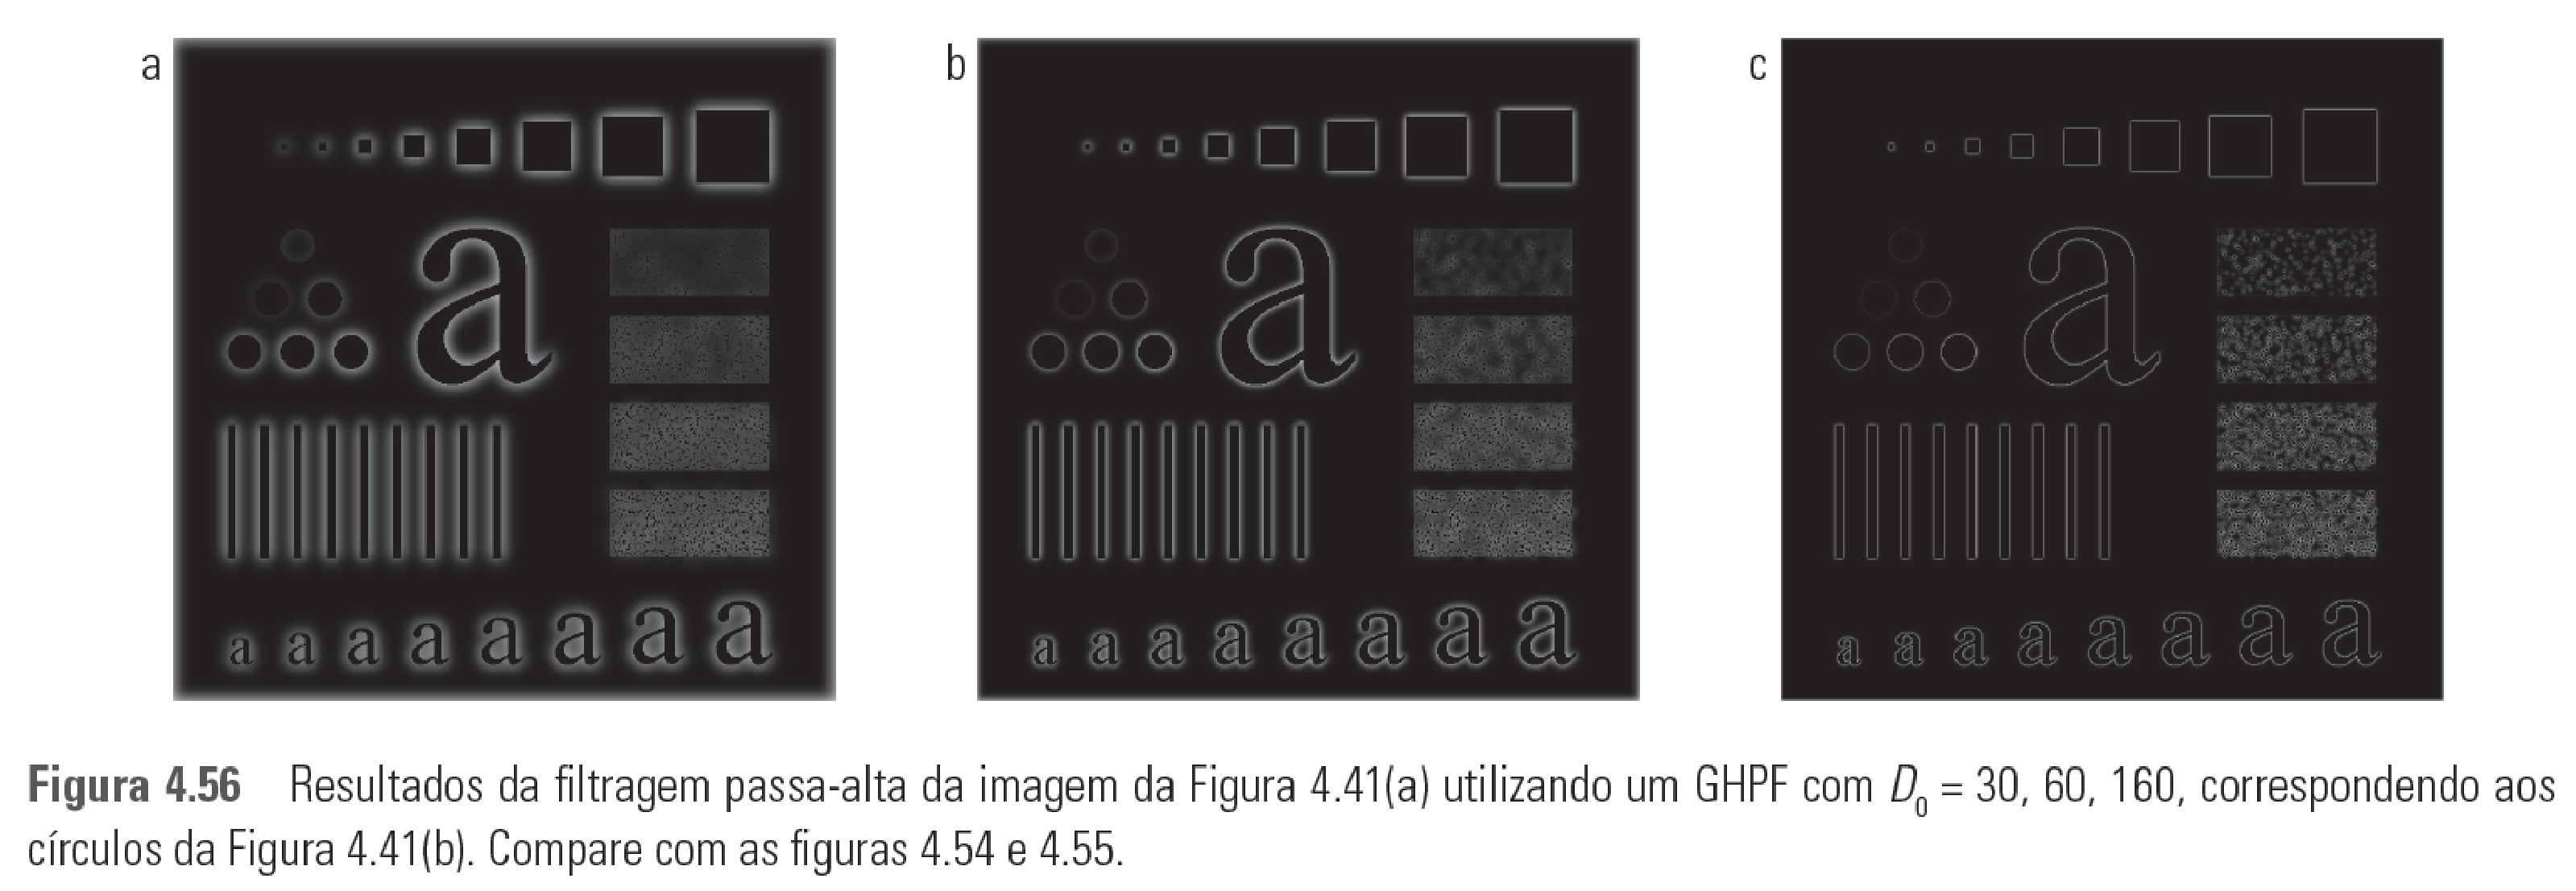
\includegraphics[width=0.65\textwidth]{figs/fig0456}
	      \end{center}
            \item Filtragem passa alta e limiarização
	      \begin{center}
            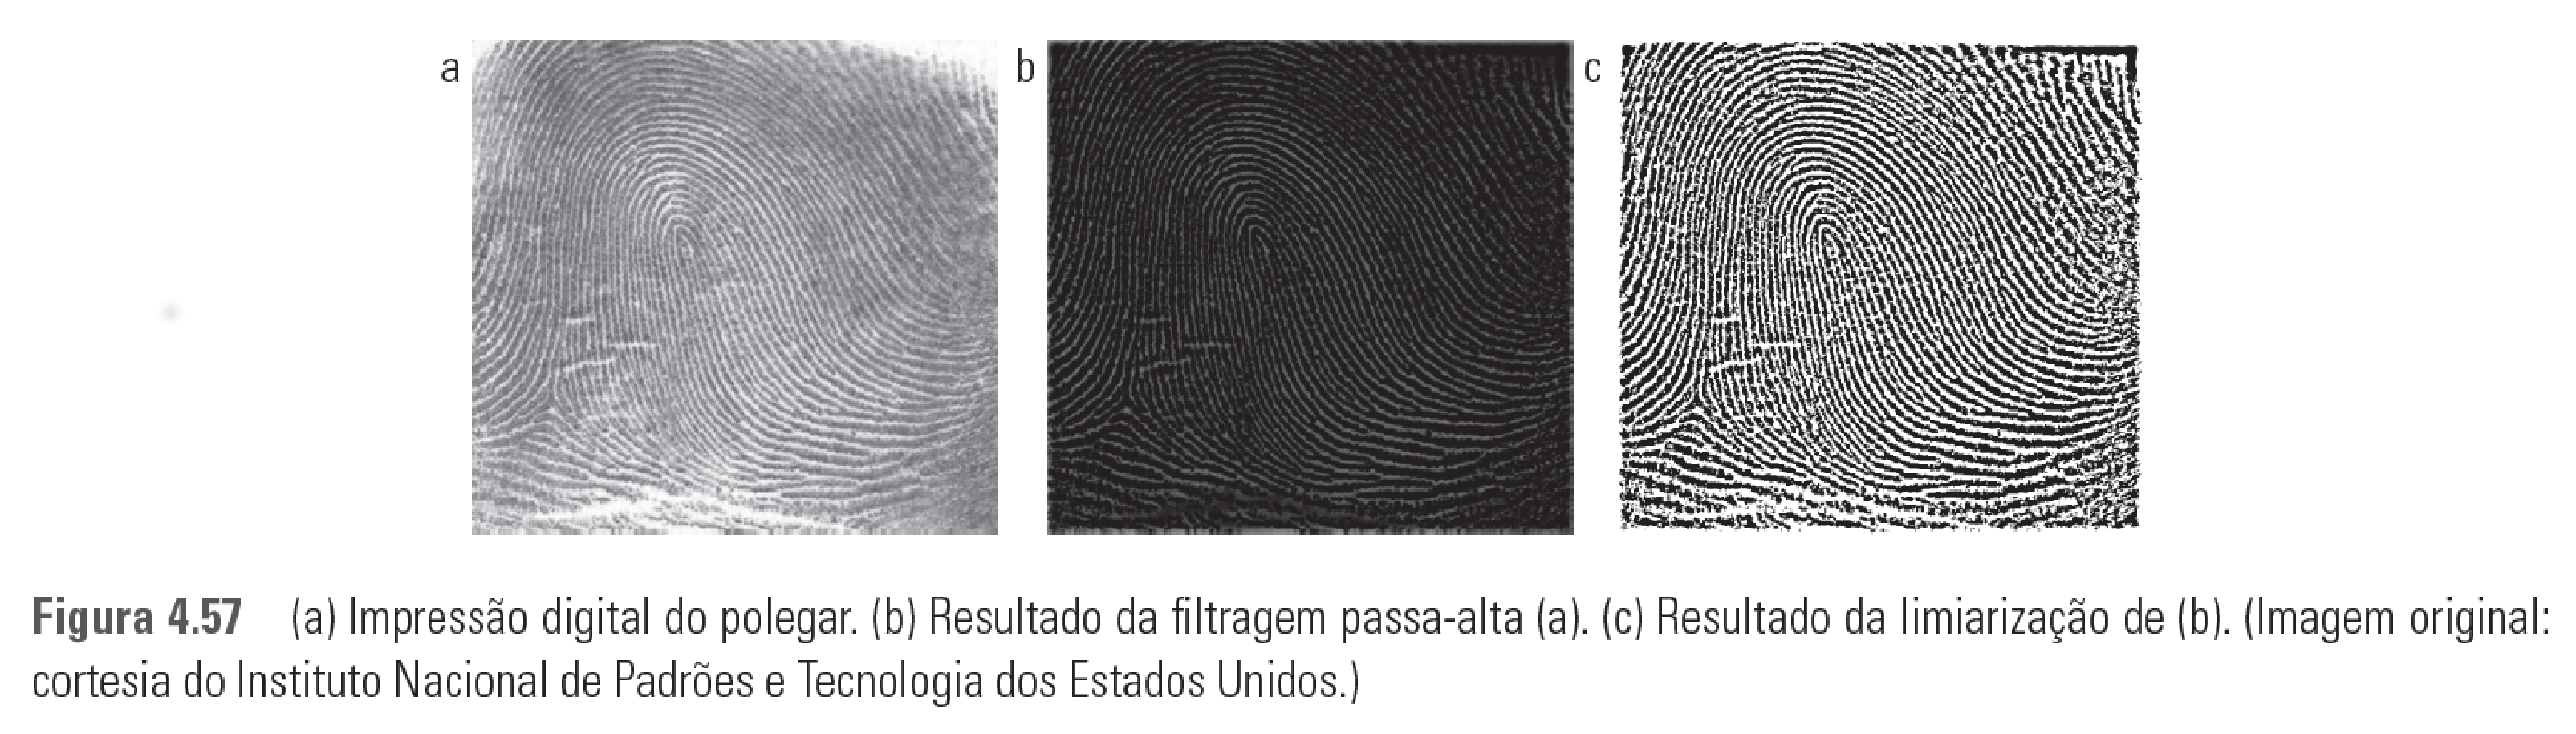
\includegraphics[width=0.65\textwidth]{figs/fig0457}
	      \end{center}
         \end{itemize}
      \end{slide}
      
      \begin{slide}[toc=]{Exemplos}
         \begin{itemize}[type=1]
            \item Radiografia de tórax
            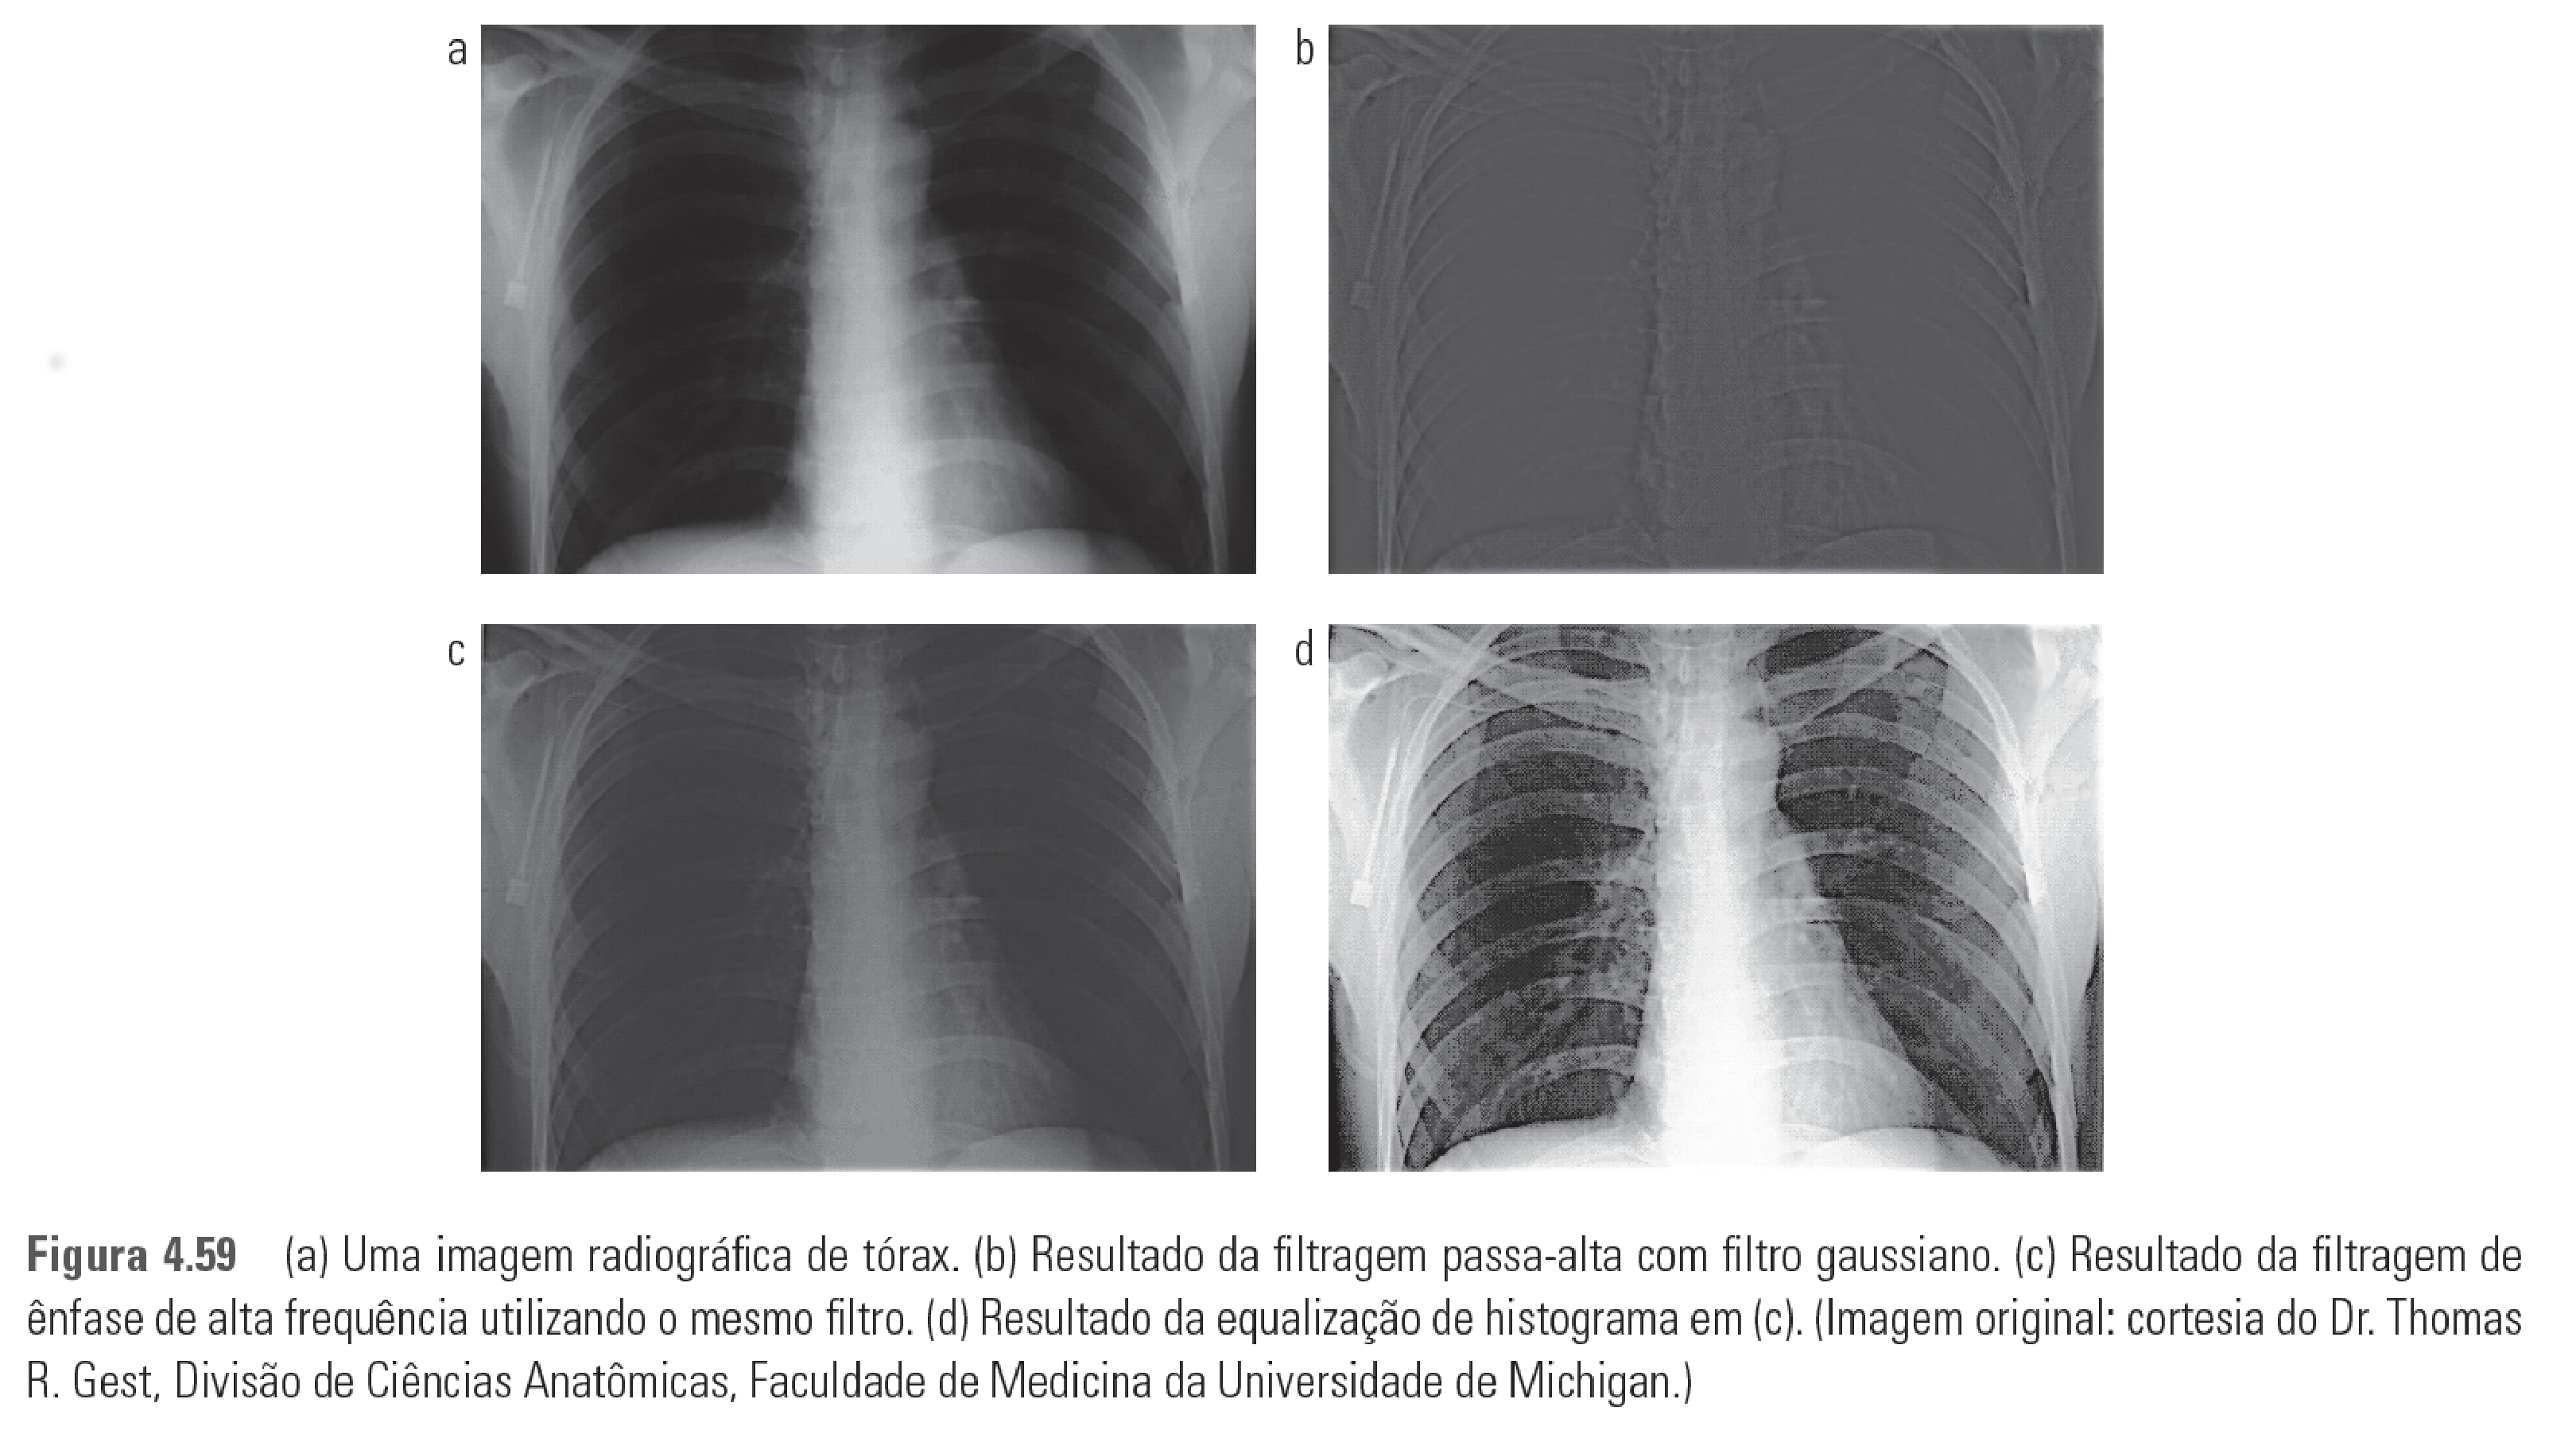
\includegraphics[width=0.95\textwidth]{figs/fig0459}
         \end{itemize}
      \end{slide}
      
   \section[slide=true]{Filtragem seletiva}
      \begin{slide}[toc=]{Filtros rejeita banda e passa banda}
         \begin{itemize}[type=1]
            \item Rejeita banda ideal
            \begin{equation*}
               H(u,v) = \begin{cases}
                           0& \text{se }|D(u,v)-D_0|\leq \frac{W}{2}\\
                           1& \text{se }|D(u,v)-D_0|>\frac{W}{2}
                        \end{cases}
            \end{equation*}
            \item Rejeita banda Butterworth
            \begin{equation*}
               H(u,v) = \frac{1}{1+\left[ \frac{D(u,v)W}{D^2(u,v)-D^2_0}\right]^{2n}}
            \end{equation*}
            \item Rejeita banda gaussiano
            \begin{equation*}
               H(u,v) = 1-e^{-\left [\frac{D^2(u,v)-D^2_0}{D(u,v)W} \right ]^2}
            \end{equation*}
            \item Passa banda: $H_{BP}(u,v) = 1-H_{BR}(u,v)$
         \end{itemize}
      \end{slide}
      
      \begin{slide}[toc=]{Filtros rejeita banda e passa banda}
         \begin{itemize}[type=1]
            \item Respostas em frequência
            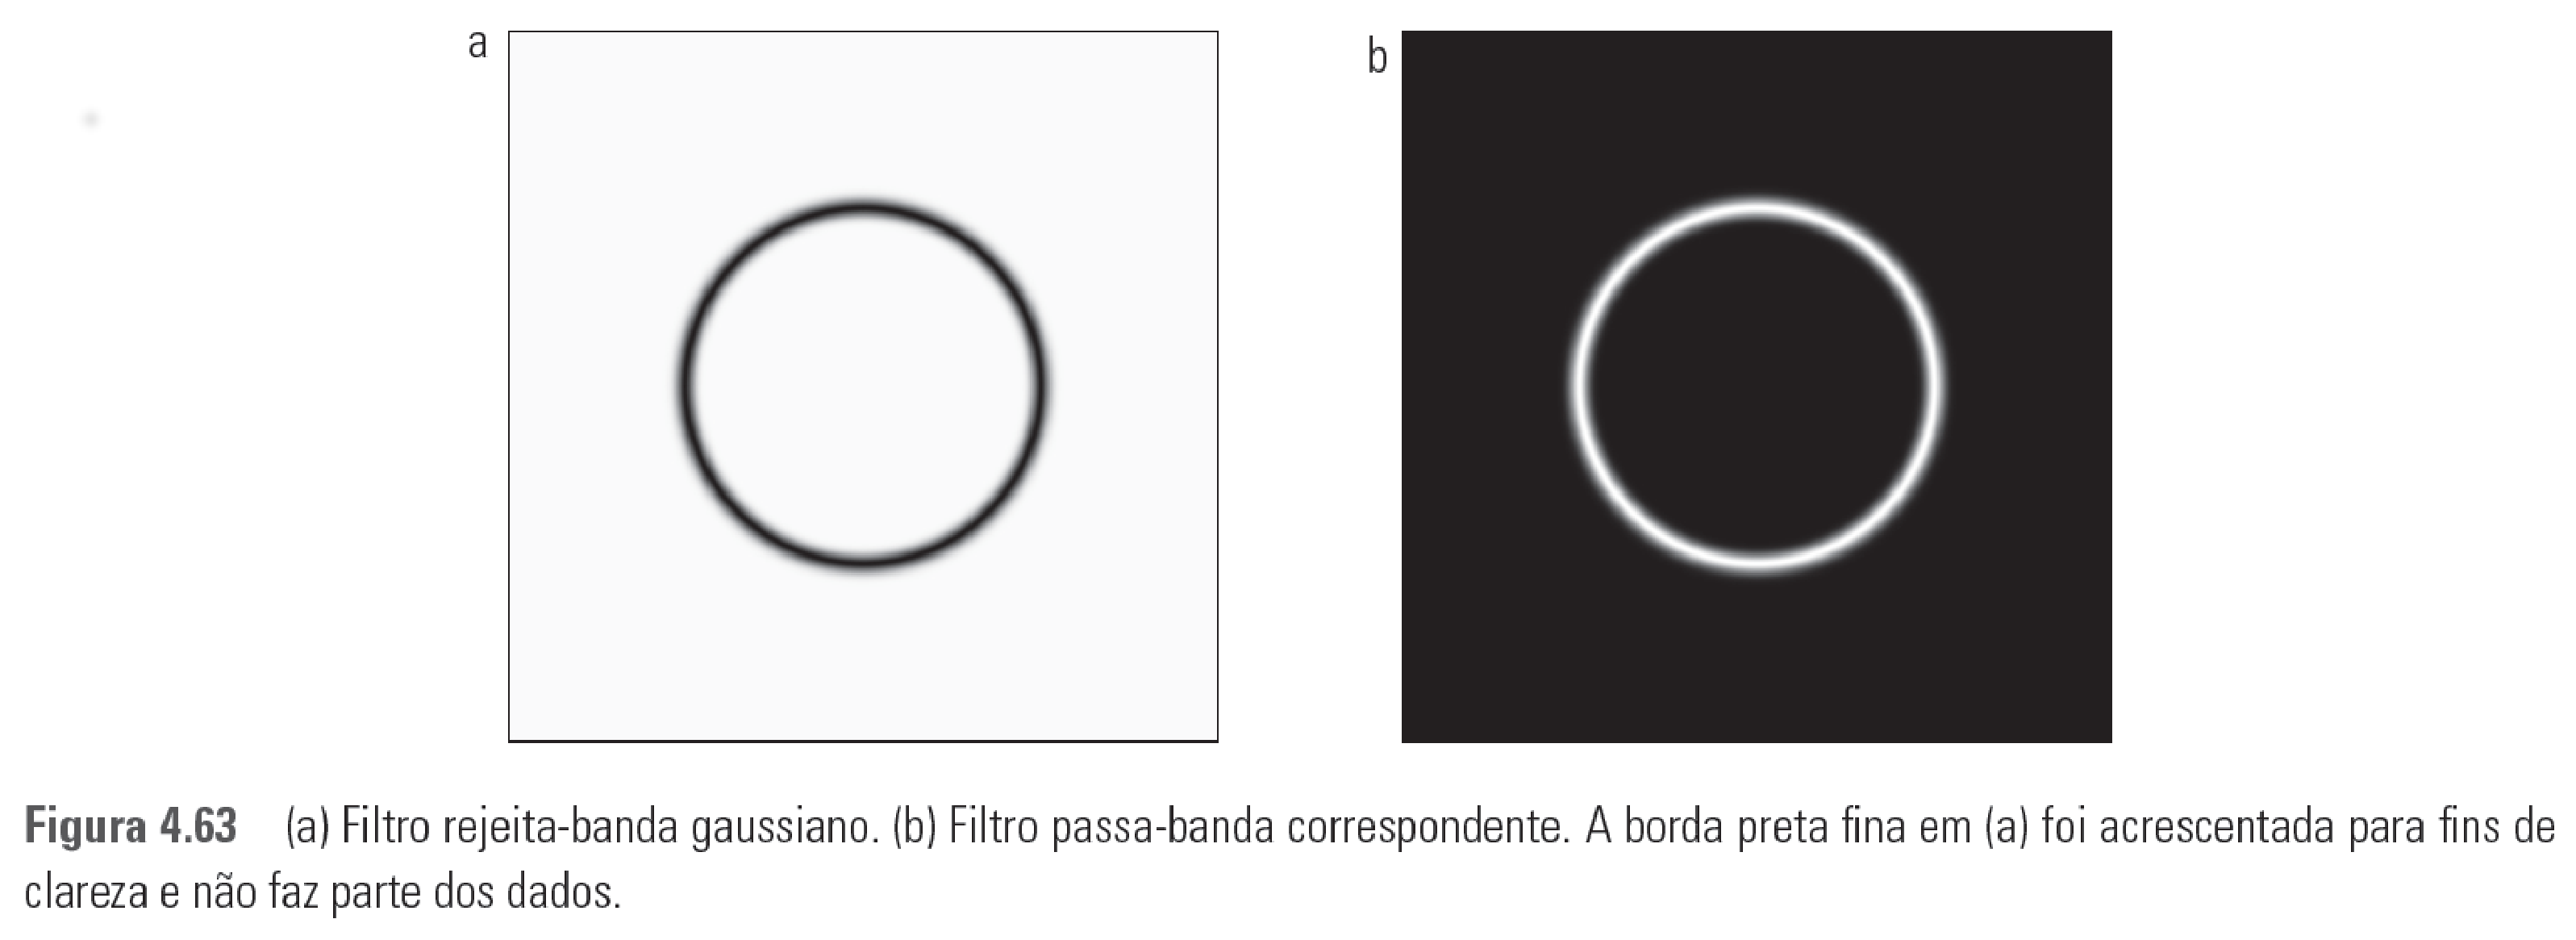
\includegraphics[width=0.95\textwidth]{figs/fig0463}
         \end{itemize}
      \end{slide}
      
      \begin{slide}[toc=]{Filtros notch}
         \begin{itemize}[type=1]
            \item Seleção (passagem ou rejeição) de frequências específicas
            \item Filtros notch de rejeição: filtros passa alta com centro transladado para 
            frequência de interesse
            \begin{equation*}
               H_{RN}(u,v) = \prod_{k=1}^Q{H_k(u,v)H_{-k}(u,v)}
            \end{equation*}
            \item Filtros notch de passagem:
            \begin{equation*}
               H_{PN}(u,v) = 1-H_{RN}(u,v)
            \end{equation*}
         \end{itemize}
      \end{slide}
      
      \begin{slide}[toc=]{Filtros notch}
         \begin{itemize}[type=1]
            \item Exemplo
		    \begin{center}
            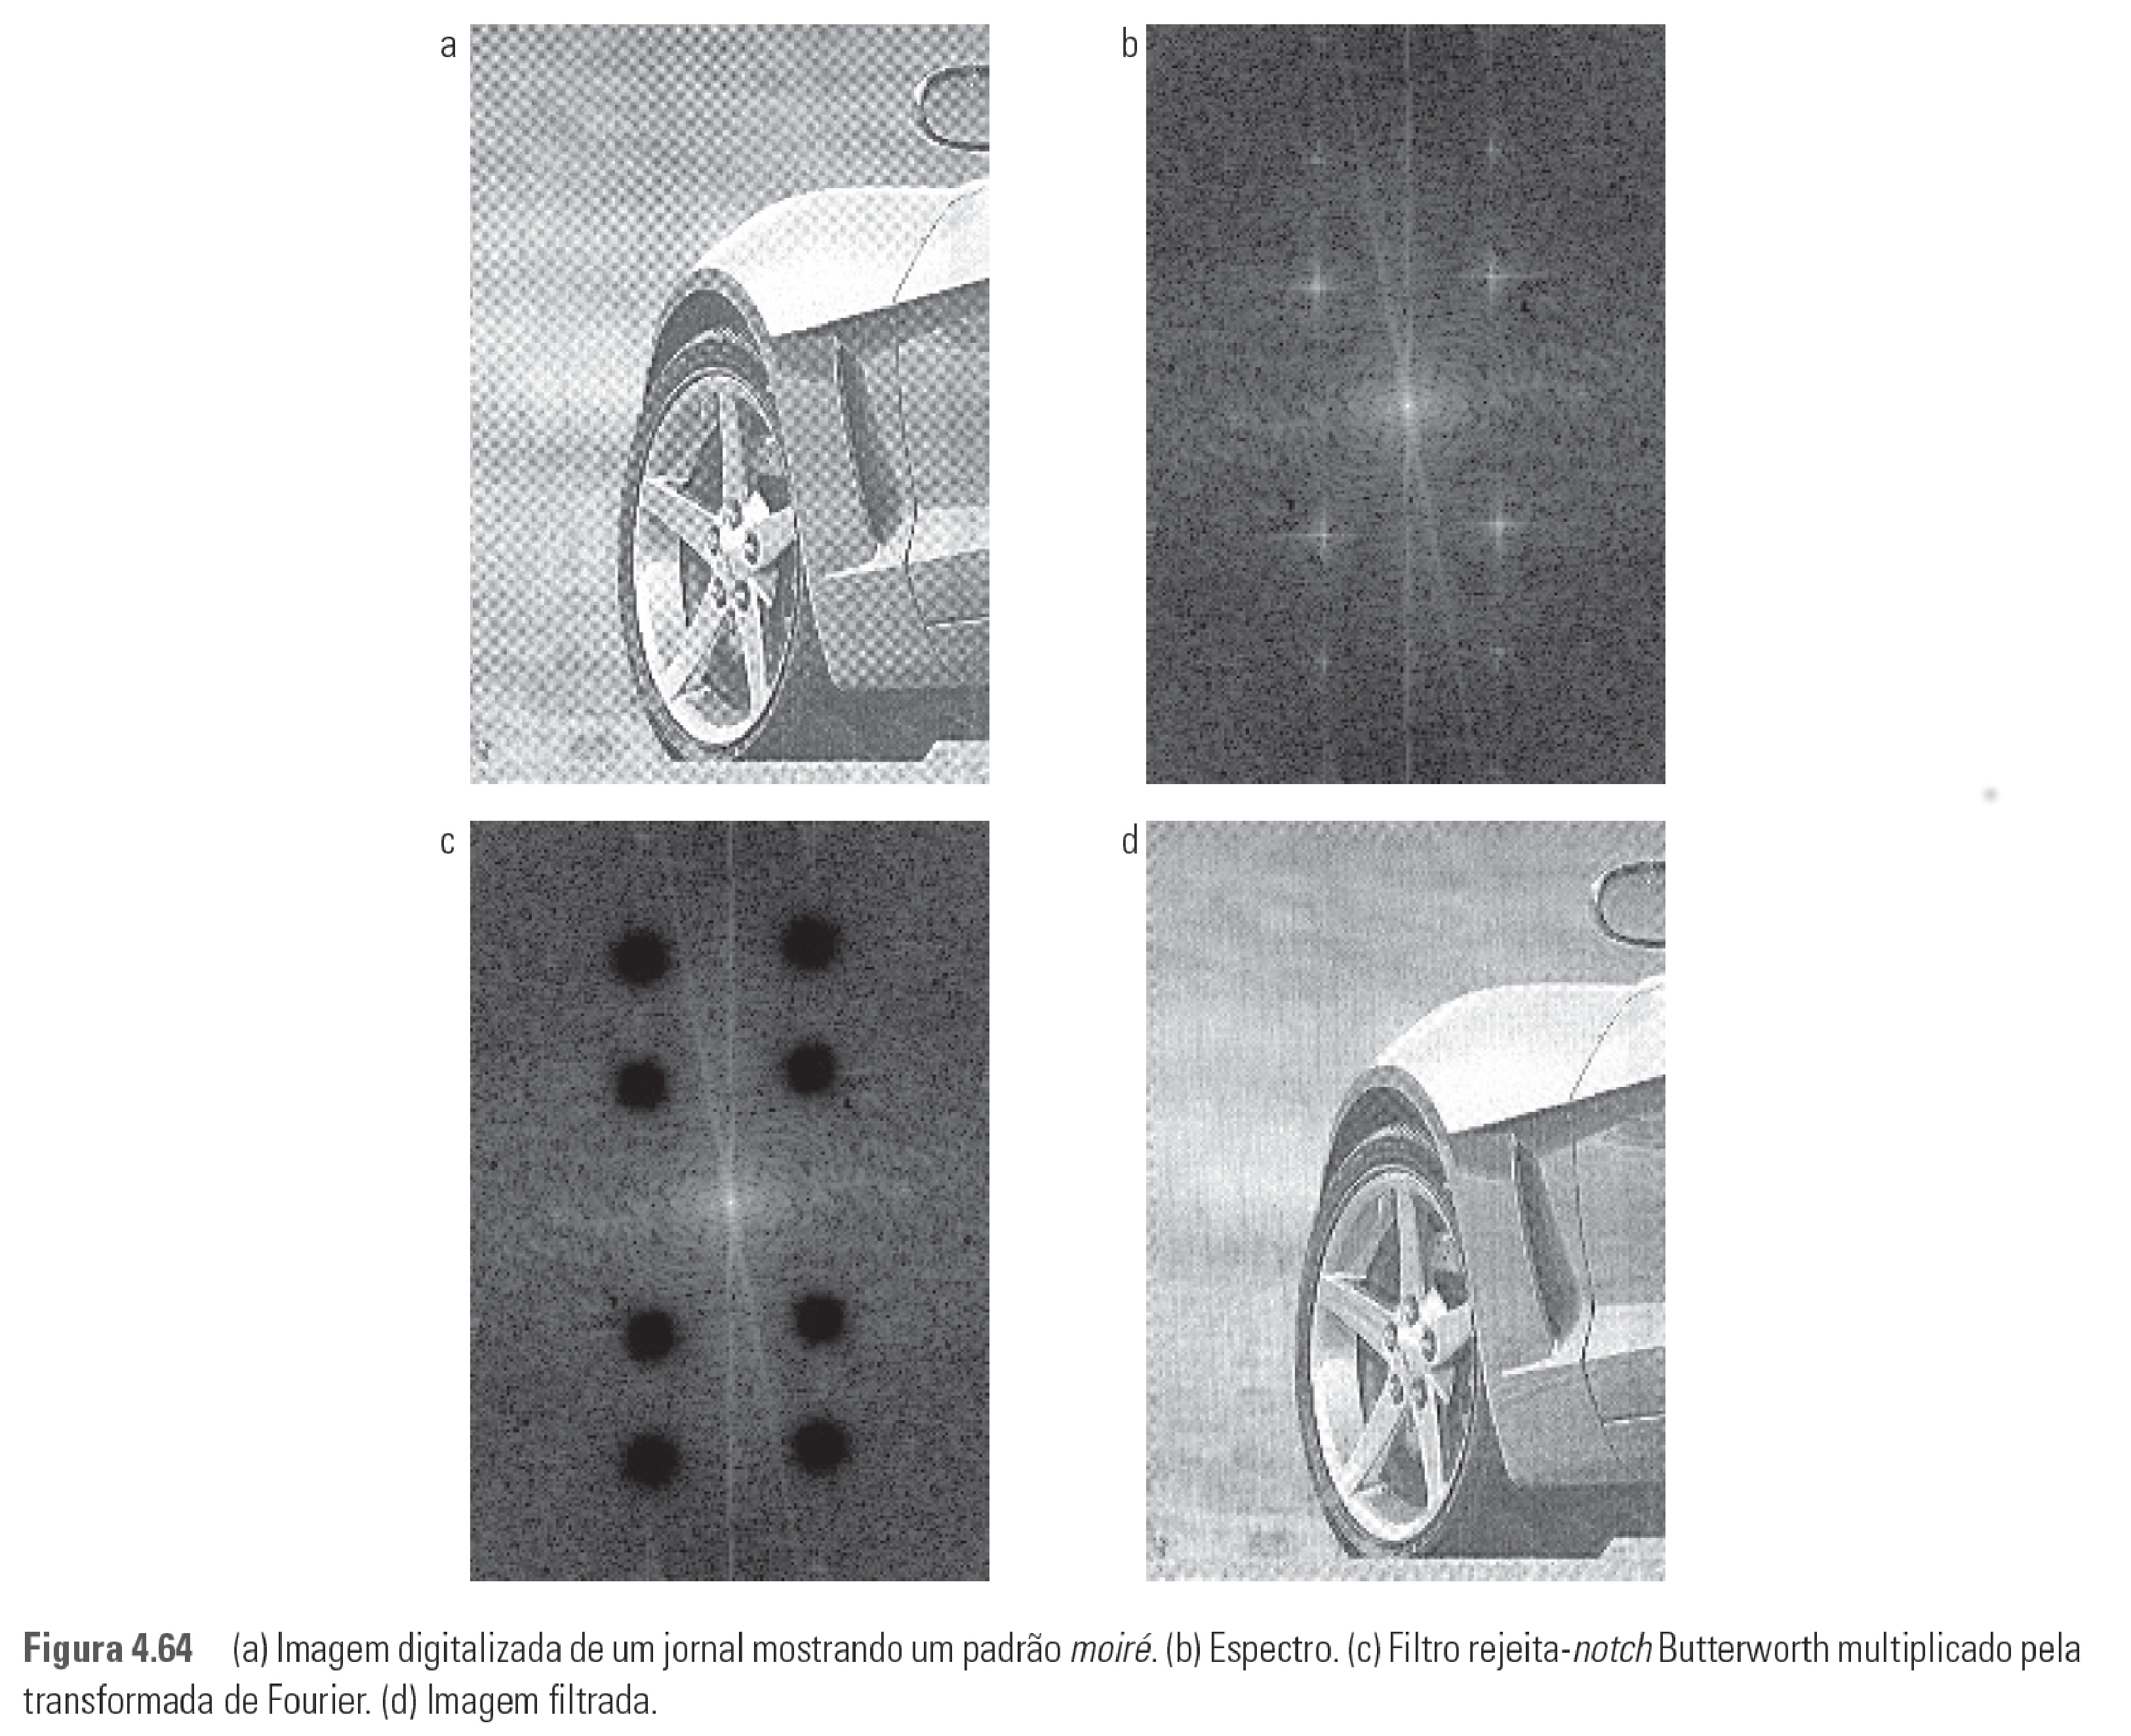
\includegraphics[width=0.6\textwidth]{figs/fig0464}
		    \end{center}
         \end{itemize}
      \end{slide}
      
      \begin{slide}[toc=]{Filtros notch}
         \begin{itemize}[type=1]
            \item Exemplo
		    \begin{center}
            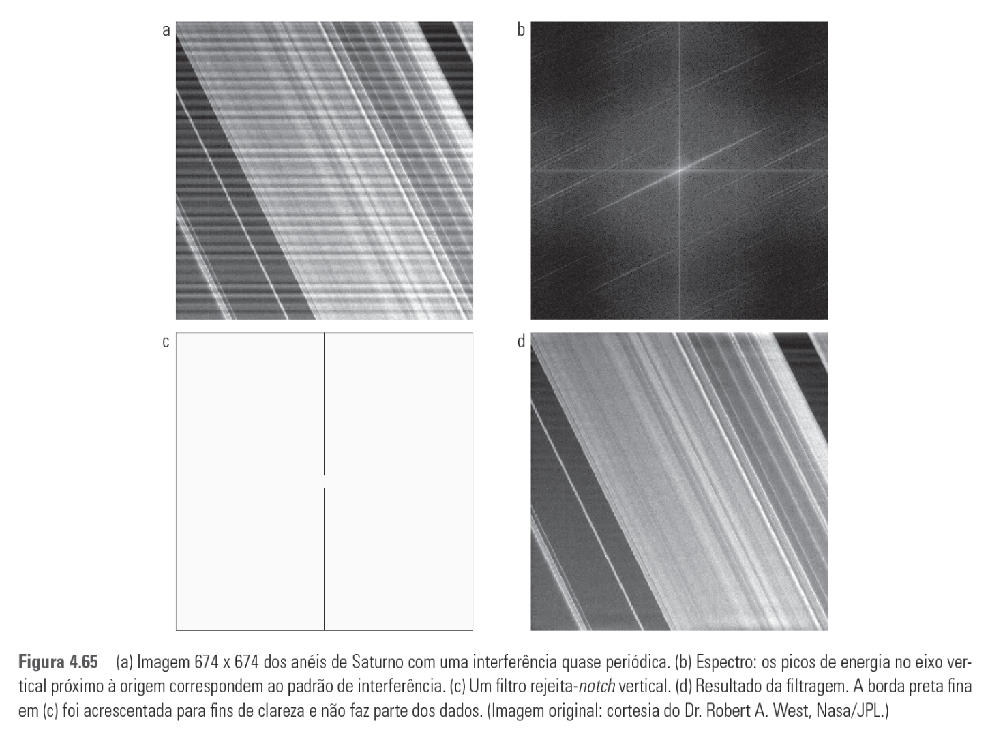
\includegraphics[width=0.7\textwidth]{figs/fig0465}
		    \end{center}
         \end{itemize}
      \end{slide}

\end{document}
